\chapter{Cross-tissue comparison of chromatin accessibility, gene expression signature and immunophenotypes in PsA}
\chaptermark{Cross-tissue comparison analysis in PsA}
\label{ch:Results3}


%%%%%%%%%%%%%%%%%%%%%%%%%%%%%%%%%%%%%%%%%%%%%%%%%%
\section{Introduction}

%The techniques to generate the scRNA-seq data have also evolved and SmartSeq2 and 10X Chromium are the two main I haven't talked at all about IL-2 and IL-8 in the relevant cytokines in disease. The reason is because they are not the mots relevant ones but due to cytof contrains they are together with TNFa and IFNg among the ones yielding the best quality results.
\subsubsection{}
PsA is considered a systemic disease where studies in PBMCs have demonstrated changes in cell type composition compared to healthy individuals. For example, increased frequencies of circulating IL-17$^+$ and IL-22$^+$ CD4$^+$ T cells have been reported in PsA PB compared to control individuals \parencite{Benham2013}. Moreover, the percentage of pDCs and NK in PB are reduced in PsA compared to controls \parencite{Jongbloed2008, Spadaro2004}. Additionally, the production of pro-inflammatory cytokines, such as IL-17 and IL-22, by stimulated PBMCs was higher in PsA than in healthy controls \parencite{Benham2013}. 

Nevertheless, PsA ischaracterised by affection of the joints, where the local inflammatory response leads to enthesitis, synovitis, bone remodelling and, eventually, joint destruction \parencite{}. The importance of studying the synovium in PsA have been highlighted by differences in cell composition and cytokine production, amongst others, between PB and SF in PsA patients. For example, expansion of CD8$^+$, mainly memory cells expressing CD45RO, was observed in SF when compared to paired PB samples \parencite{Ross2000}. Additionally, the elevated proportion of T cells expressing the cytokine receptors CCR6$^+$ and IL-23R$^+$ were found in SF compared to PB \parencite{Benham2013}. Patients presenting oligoarticular PsA (involving four or fewer joints) are usually na\"{i}ve for biologic treatments (only NSAIDs) and this PsA manifestation is commonly managed by joint aspiration prior intra-articular steroid injection to relieve pain, being particularly convenient for SF sample collection \parencite{Kavanaugh2006}.


% Differences between bulk PB and SF in terms of cell composition-and transcriptomics-explain some findings
% Transcriptome differences examples

Initially, genome-wide transcriptomic studies have focused in characterising gene expression in bulk PBMCs and SFMCs samples. Several studies have been conducted to better understand differences in gene expression at the systemic level between PsA and controls, tissue-specific differences comparing paired PB and SF from PsA patients and comparison across other SpA and arthritic diseases \parencite{Stoeckman2006, Batiwalla2005, Gu2002, Dolcino2015}. Amongst the more comprehensive studies is the conducted by Dolcino and colleagues revealing differentially expressed genes in the Th-17 axis and type-I IFN signalling in PsA synovial membrane biopsies compared to healthy ones. Moreover, comparison between the DEGs in both PsA compartments when compared to healthy controls, highlighted differences and commonalities in the systemic and tissue PsA immune response. Other studies have also focused in the understanding the transcriptional changes in PBMCs from PsA patients following MTX and TNFi therapies \parencite{Cuchacovich2014}. Likewise, measurement of cytokines production have also been conducted in serum and SF, revealing increased levels of TNF-$\alpha$, for example, in both tissues \parencite{Ritchlin1999,Li2017}. 

Consideration of cell and type specificity in the study of complex diseases has enabled a better understanding of the disease pathophysiology. The molecular characterisation of the different immune cell types is pivotal not only for the understanding of the immune response but also to define disease state, understand the impact of genetic variants increasing disease risk and the identify of drugs optimal efficacy and specificity. For example, the importance of considering cell types to understand the impact of genetic variants in transcriptional regulation has been explored in a number of immune cells \parencite{eQTL}. These studies have highlighted the regulatory role of some genetic variants only in particular cell types and conditions, previously masked when considering mixed population of cells such as PBMCs. % any other reference to bulks or mixed pop? 
In this respect, expression analysis for a limited number of genes have been performed in specific cell type populations such as stimulated macrophages and Th-17 \textit{in vitro} differentiated cells from na\"{i}ve CD4$^+$ isolated from PB and SF of PsA patients \parencite{Antoniv2006, Leipe2010}. Overall, achieving a detailed and precise understanding of complex diseases requires the study of sorted cell populations and when possible isolated from the affected tissue.  



%Downside of bulk versus cell type specific and further sc
-Some differences masked at the transcriptional level
-Loss of information about relevance of each cell type in the pathophysiology



\subsubsection{Multi-omics}
- Link to the importance of context specificity in complex diseases 
	-Environment
	-Genetic
	are both affected by Epigenetics which is very dynamic and cell and tissue specific
	
	-In order to have a general understanding of disease state and also to better contextualise the functional role of genetic variants a cell and tissue specific approach is needed
	
	-ATAC: examples of some studies in other disease. No studies in PsA
	-Gene expression and some studies linking both ATAC and gene expression
	-scRNA 
	-Final impact on the protein (CyTOF)
	Immunophenotypes
Differences in genes expression were also studied between pDCs and mDCs isolated from both PsA tissues
Jongbloed2008
as well as in synoviocytes (FLS) obtained from synovial tissues Raychaudhuri
	
	-Integration including fine-mapping (look at previous paper from Hussein)
	
	-Hole in the field
	
	
	\subsection{Aims}











%%%%%%%%%%%%%%%%%%%%%%%%%%%%%%%%%%%%%%%%%%%%%%%%%%
\section{Results}
%

\subsection{PsA patients cohort description and datasets}
In this study peripheral blood (PB) and SF were collected from a cohort of six PsA patients, with equal numbers of males and females (Table \ref{tab:PSA_cohort_metadata}). All the patients presented oligoarticular joint affection and had been first diagnosed with psoriasis. The cohort presented a mean of 1.5 tender or swollen affected joints (TJC66 and SJC66), which is characteristic of the oligoarticular form of disease (involving four or fewer joints). Regarding global assessment, the mean scores for the patient and physician evaluation were X and 3, respectively, in a scale of 1 to 5. These four measurements including joints and global assessment compose the PsARC disease activity scores, used by clinicians as the main indicator of response to treatment by recommendation of the National Institute for Health and Care Excellence (NICE) (Chapter \ref{ch:Intro}). 

The mean age of the cohort at the time of diagnosis was 44.3 years old and the mean disease duration 8.8 years. Interestingly, PsA1728 was diagnosed at a later age compared to the other patients in the cohort (late PsA onset clinical significance??). Moreover, C-reactive protein (CRP) levels, other marker of inflammation, presented an average of 17.45 mg/L and was particularly higher in PsA1719 and PsA1728 compared to the other patients. At the time of sample recruitment all the PsA patients were na\"{i}ve for treatment and only PsA1505 had been on MTX therapy in the past for xxx months/years (how many years ago?). Post-visit, most of the patients qualified for TNAi biologic therapy xxxx.


%
\begin{landscape}
\begin{center}
\begin{longtable}[ht]{c c c c c c c c c}
%{p{.15\textheight} p{.15\textheight} p{.25\textheight} p{.25\textheight} p{.15\textheight} p{.15\textheight} p{.15\textheight}}
\caption[Description of PsA patients cohort recruitment and metadata.]{\textbf{Description of PsA patients cohort recruitment and metadata.}. PsARC disease activity score is composed of tender joint count 66 (TJC66) and swollen joint count 66 (SJC66), joint pain (4 point score) and self-patient and physician global assessment (5 point score). Joint pain and global assessment use a likert scale based on questionnaire answers that measure the level of agreement with each of statements included. C-reactive protein (CRP).}
\label{tab:PSA_cohort_metadata} \\
\toprule
\textbf{ Sample ID} & \textbf{Sex} & \textbf{Age at} & \textbf{Disease duration} & \textbf{Type} &\textbf{TJC66/SJC66}  & \textbf{Physician } & \textbf{Patient} & \textbf{CRP} \\
                   &               & \textbf{diagnosis} & \textbf{(months)}      &               &                      & \textbf{assessment} & \textbf{assessment}  & \textbf{(mg/L)} \\
\midrule
\midrule
PsA1718 & Female & 17 & 180 & Oligo  & 2/2 & 3 & 3 & 6 \\
PsA1719	& Male &	33 & 24	 & Oligo &	1/1 &	3 & 4 & 36.6 \\           
PsA1607 &	Male & 42 & 108 &	Oligo &	1/1	& 4 & 3 & 8 \\
PsA1728	& Female & 72	& 48 & Oligo & 2/2 & 3 & 4 & 43.2 \\
PsA1801	& Female & 53 & 168 & Oligo & 2/2 &	3 & 3 & 9.9 \\
PsA1505 & Male & 35 &	108 & Oligo & 1/1 & 2 & 2 & 1 \\	
\midrule
Total		& $-$	&	44.3 & 106 & $-$ & 1.5/1.5 & 3 & 3.2 & 17.45 \\																			
\bottomrule
\medskip
\end{longtable}
\end{center}
\end{landscape}

%\clearpage

For each of the patients, paired data in PB and SF was generated from bulk mononuclear cells or specific isolated cell types of interest (detailed in Table \ref{tab:PSA_datasets_per_sample} and Chapter \ref{ch:Mat}). Due to project contrains, ATAC-seq, PCR gene expression array, scRNA-seq and mass cytometry were not generated for all six individuals in the cohort. 

\begin{table}[htbp]
%\setlength{\tabcolsep}{20pt} only to stretch the columns if you want
%\renewcommand{\arraystretch}{1.5}
\centering
\begin{tabular}{@{} c c c c c}
\toprule
\textbf{Sample ID} & \textbf{\% FAST-ATAC} & \textbf{RNA PCR array} & \textbf{scRNA-seq} & \textbf{Mass cytometry} \\
\midrule
\midrule
PsA1718 & Yes & No & No & Yes\\
PsA1719 & Yes & Yes & No & Yes\\
PsA1607 & Yes & Yes & Yes & Yes\\
PsA1728 & No & Yes & No & No\\
PsA1801 & No & No & Yes & No\\
PsA1605 & No & No & Yes & No\\
\bottomrule
\end{tabular}
\medskip %gap
\caption[Datasets generated for the PsA cohort samples.]{\textbf{Datasets generated for the PsA cohort samples.} Four types of data were generated in a paired way between PB and SF from the same individual. The available data sets vary between individuals due to project constrains. FAST-ATAC data was generated for CD14$^+$, mCD4$^+$,mCD8$^+$ and NK cells. RNA expression by PCR array was performed for CD14$^+$, mCD4$^+$ and mCD8$^+$. scRNA-seq data was generated using 10X technology in bulk PBMCs, bulk SFMCs and sorted mCD4$^+$ and mCD8$^+$ isolated from both tissues.}
\label{tab:PSA_datasets_per_sample}
\end{table}
\bigskip %bigger space

\subsection{Immune cellular composition of blood and synovial fluid in the PsA cohort}
The immune cellular composition of three PsA samples (PsA1718, PsA1719 and PsA1607) was characterised in SF and PB using the ICS mass cytometry panel in Chapter \ref{ch:Mat}. For both tissues, mCD4$^+$ (between 32.1 and 55.6\%) constituted the most abundant cell type followed by mCD8$^+$ (between 16.9 and 24.9\%) and CD14$^+$ "non-classical" monocytes (between 6.9 and 21.7\%). Consistently with previous studies, a trend of increased percentage of mCD8$^+$ pDCs and cDCs were observed in SF compared to PB \parencite{Ross2000,Jongbloed2006}. Interestingly, this data also showed reduced circulating NK cell percentage compared to controls, in the same lines as previous studies suggesting the role of impaired non-MHC-restricted cytotoxicity in PsA \parencite{Spadaro2014}. Similarly, a tendency towards reduced proportions of B cells  in SF compared to PB reinforced the lack of contribution of the humoral immune response in PsA pathophysiology \parencite{}. The observed differences cell composition between SF and PB were not statistically significant for any of the twelve analysed populations likely due to the small samples size (only three individuals) available for the analysis. Further increase in the sample size will probably proof statistical statistical significance for the observed differences in immune cell composition between the two tissues in lines with the results published by other studies.   

% Add the markers used to define each of the cell types and calculation of percentages based on the the total number of cells in the cluster
\begin{figure}[H]
\centering
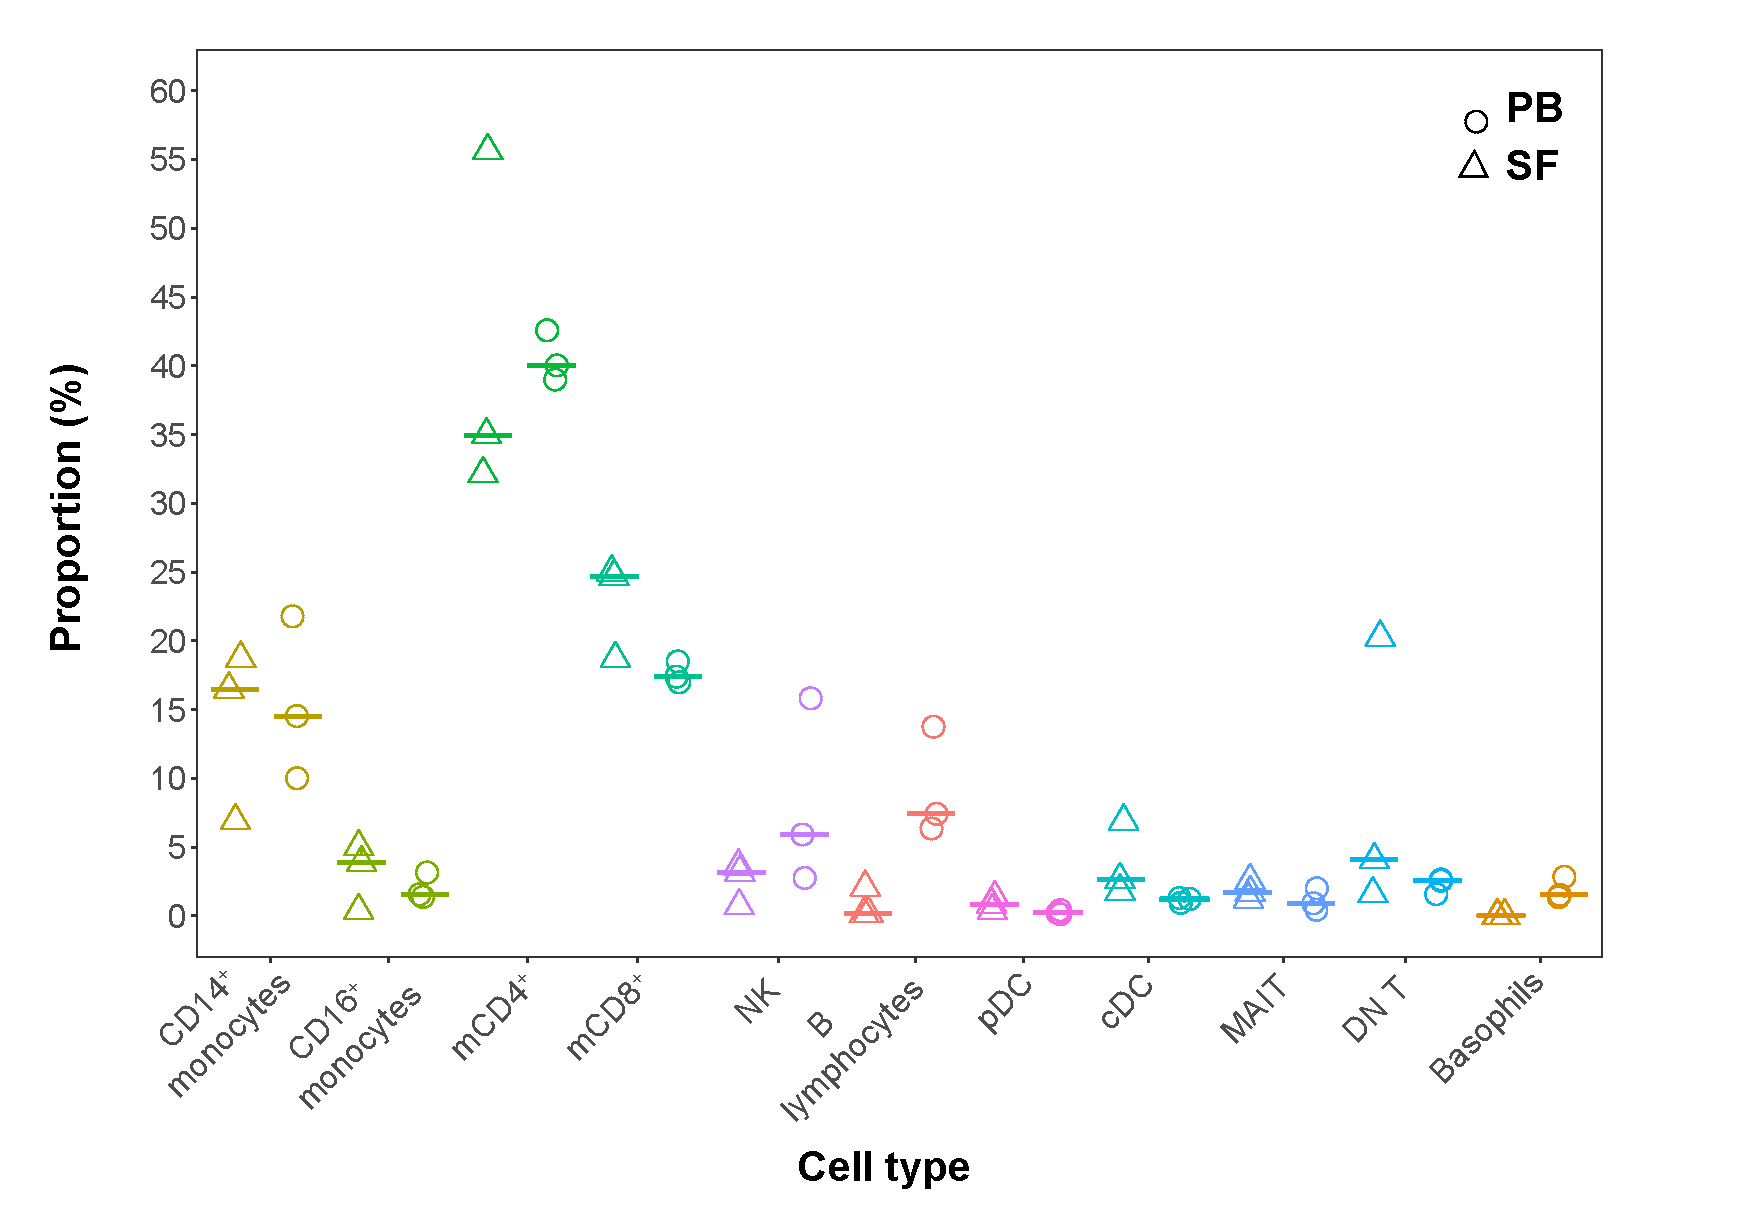
\includegraphics[width=0.7\textwidth]{./Results3/pdfs/PSA_ATAC_cohort_cell_type_composition_boxplots}
\caption[Comparative percentages of PB and SF immune cellular composition from the PsA cohort.]{\textbf{Comparative percentages of PB and SF immune cellular composition from the PsA cohort.} Percentages of each of the twelve cell types identified by mass cytometry are shown by individual and tissue for PsA1718, PsA1719 and PsA1607. Horizontal line represents the median percentage for a particular cell type in the appropriate tissue (SF or PB). Each of the cell types is displayed in a different colour. Central DC=cDC, mucosal-associated invariant T=MAIT, DN=double negative.)}
\label{figure:PsA_cell_composition}
\end{figure}



\subsection{Chromatin accessibility differential analysis in immune cells reveals differences between SF and PB}

\subsubsection{Quality control of open chromatin regions}
The twenty four FAST-ATAC PsA samples from four different cell types and two tissues (PB and SF) were sequenced to a median of 158M reads (79M paired-end) per sample. After filtering for low quality mapping, duplicates and MT reads, the median total number of reads ranged between 46.6 and 70.2 M reads, upon cell type (Figure \ref{figure:PsA_FAST_ATAC_QC} a).  Overall, MT and duplicated reads accounted for a median between 40 to 62.2\% of the total number of reads depending on cell type (Figure \ref{figure:PsA_FAST_ATAC_QC} b) and importantly contributing to the loss of reads FAST-ATAC. The final number of reads remaining after filtering was inversely related to the percentage of MT and duplicated reads identified. For example, mCD14$^+$ and mCD8$^+$ presented the lowest median of total number of reads after filtering concomitantly with the greatest percentage of combined MT and duplicated reads. 
%As previously mentioned, the MT DNA in ATAC-seq is one of the main sources of read loss, which is more accessible to the Tn5 transposase due to the absence of nucleosomes. Although the FAST-ATAC protocol represented an improvement, the percentage of MT reads across amongst all the samples ranged between 2.1 and 25.4\%. Similarly, despite initial optimisation of the number of PCR cycles used in the library amplification, the duplicated reads still represented between 22.9 to 55\% of the total number sequenced reads.

Regarding sample quality, TSS enrichment analysis showed differences in the levels of background noise across cell types and highlighted the variability of FAST-ATAC performance (Figure \ref{figure:PsA_FAST_ATAC_QC} c). A trend towards greater TSS enrichment in PB samples compared to SF was observed in all four cell types. mCD4$^+$ and mCD8$^+$ presented the best signal-to-noise ratios, with median of 19.1 and 23.1 fold enrichment, respectively. In contrast, NK was the cell type with the lowest TSS enrichment values. Particularly, the fold enrichment for PsA1719 and PsA1607 were 7.3 and 6.2, respectively, both just above the 6 to 10 acceptable range from ENCODE. If a larger cohort size was available these two samples would be removed from the differential analysis, since high background levels can reduce the power of this approach. 

 
\bigskip
\begin{figure}[H]
\centering
\begin{subfigure}[b]{0.48\textwidth}
\centering 
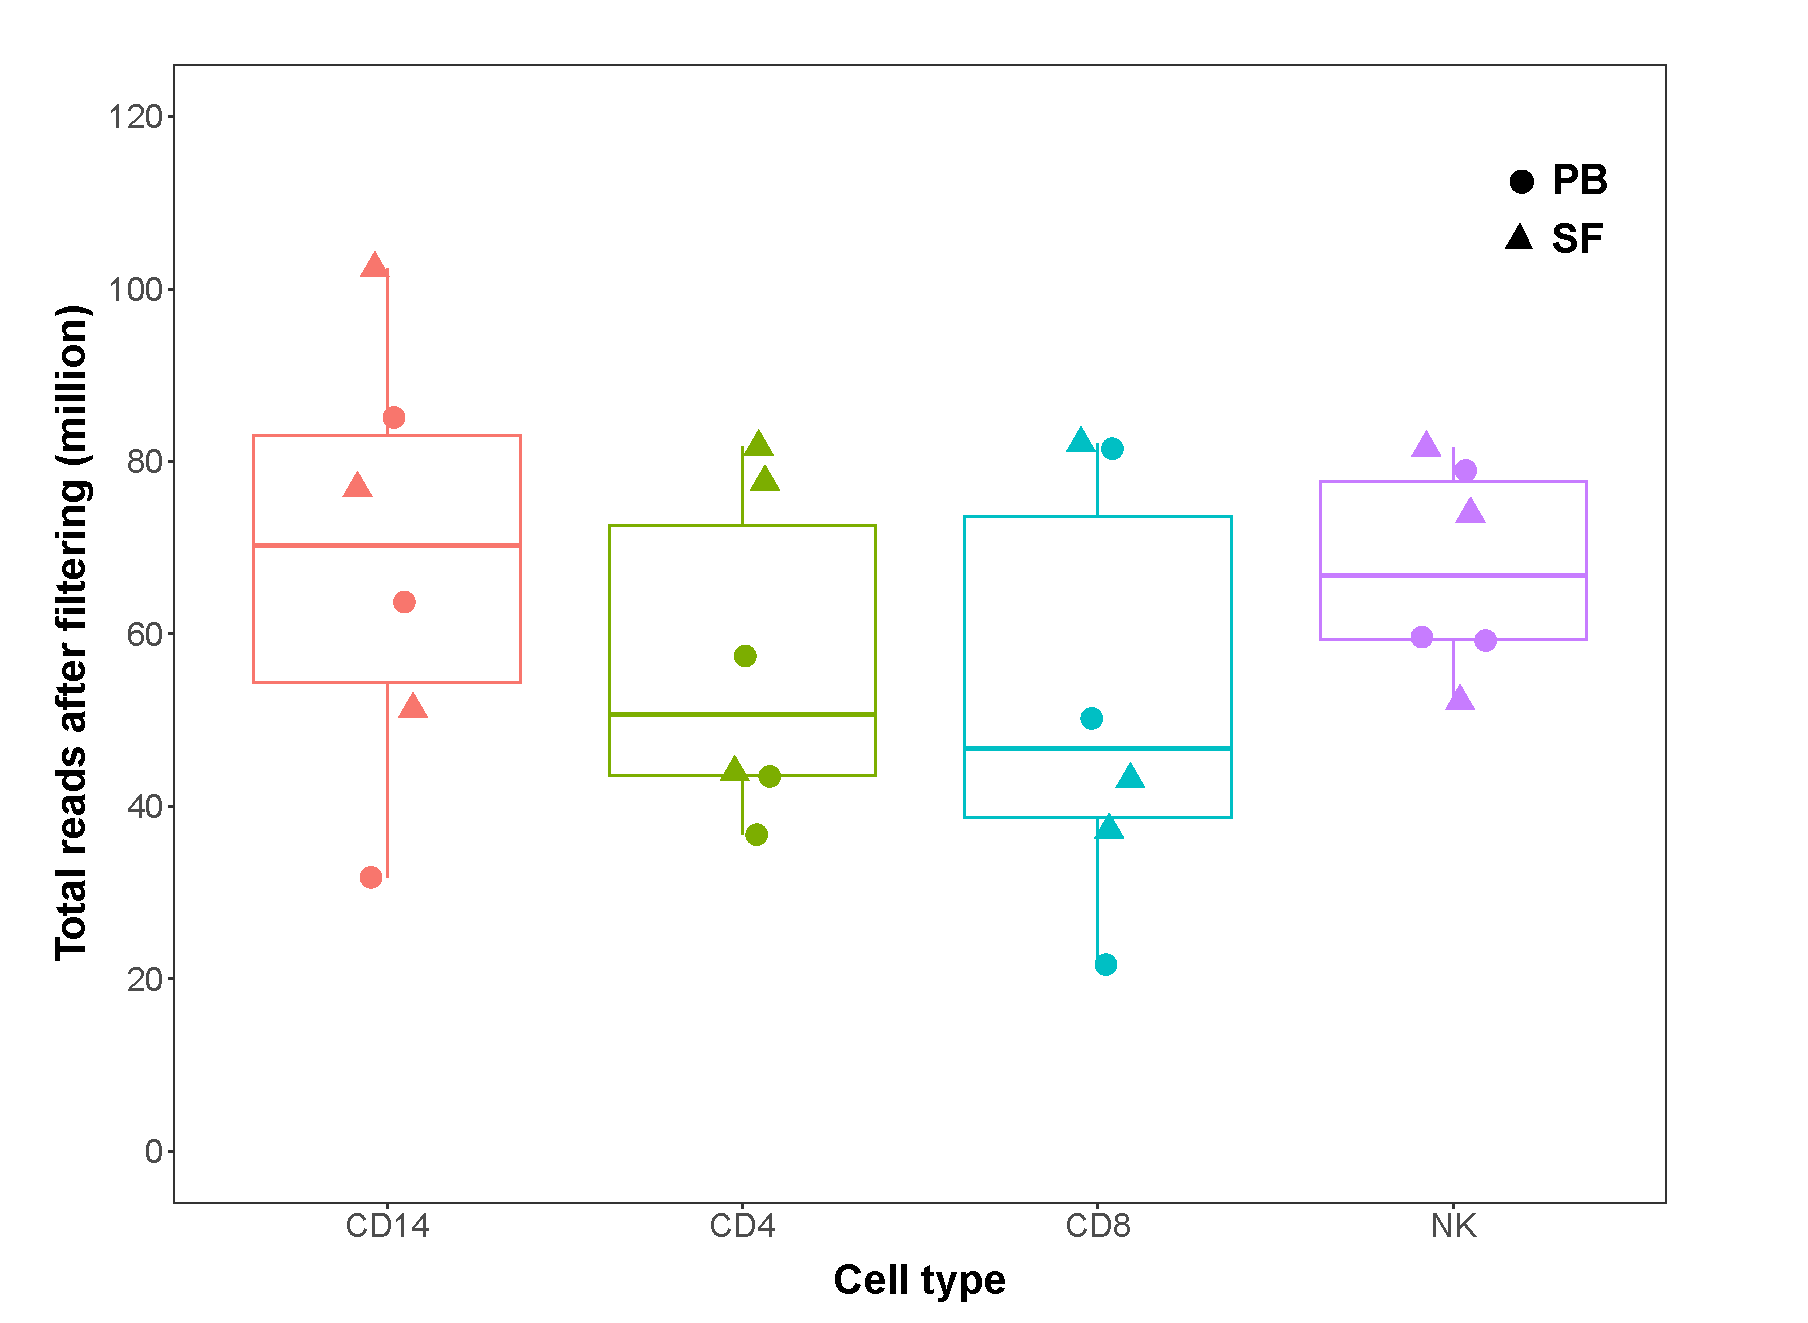
\includegraphics[width=\textwidth]{./Results3/pdfs/ATAC_PSA_total_filtered_reads_boxplot}
\caption{}
\end{subfigure}
~
\begin{subfigure}[b]{0.48\textwidth}
\centering 
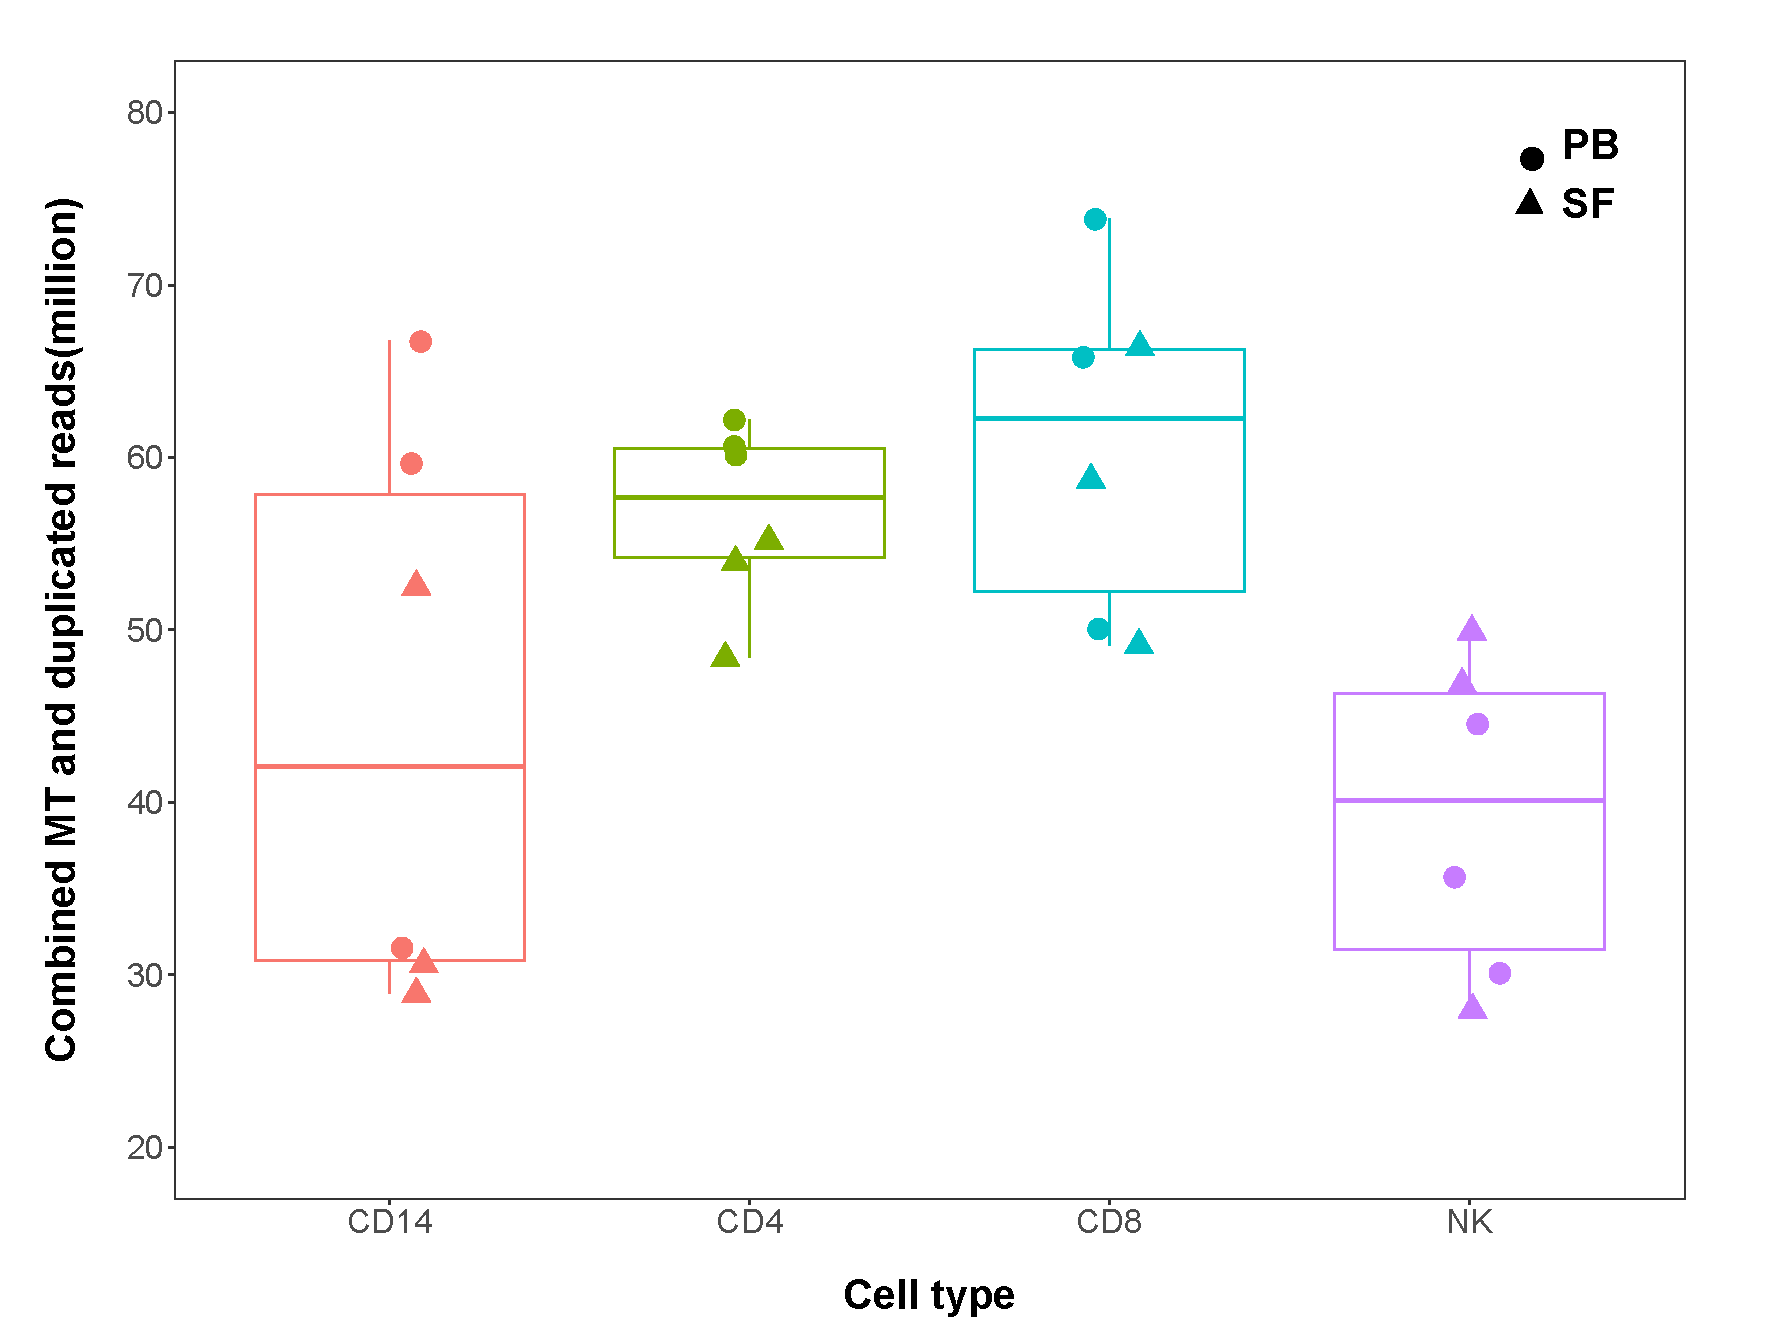
\includegraphics[width=\textwidth]{./Results3/pdfs/ATAC_PSA_pcnt_dups_and_MT_reads_boxplot}
\caption{}
\end{subfigure}
~
\begin{subfigure}[b]{0.48\textwidth} 
%the [b] prevents offset in subcaptions
\centering
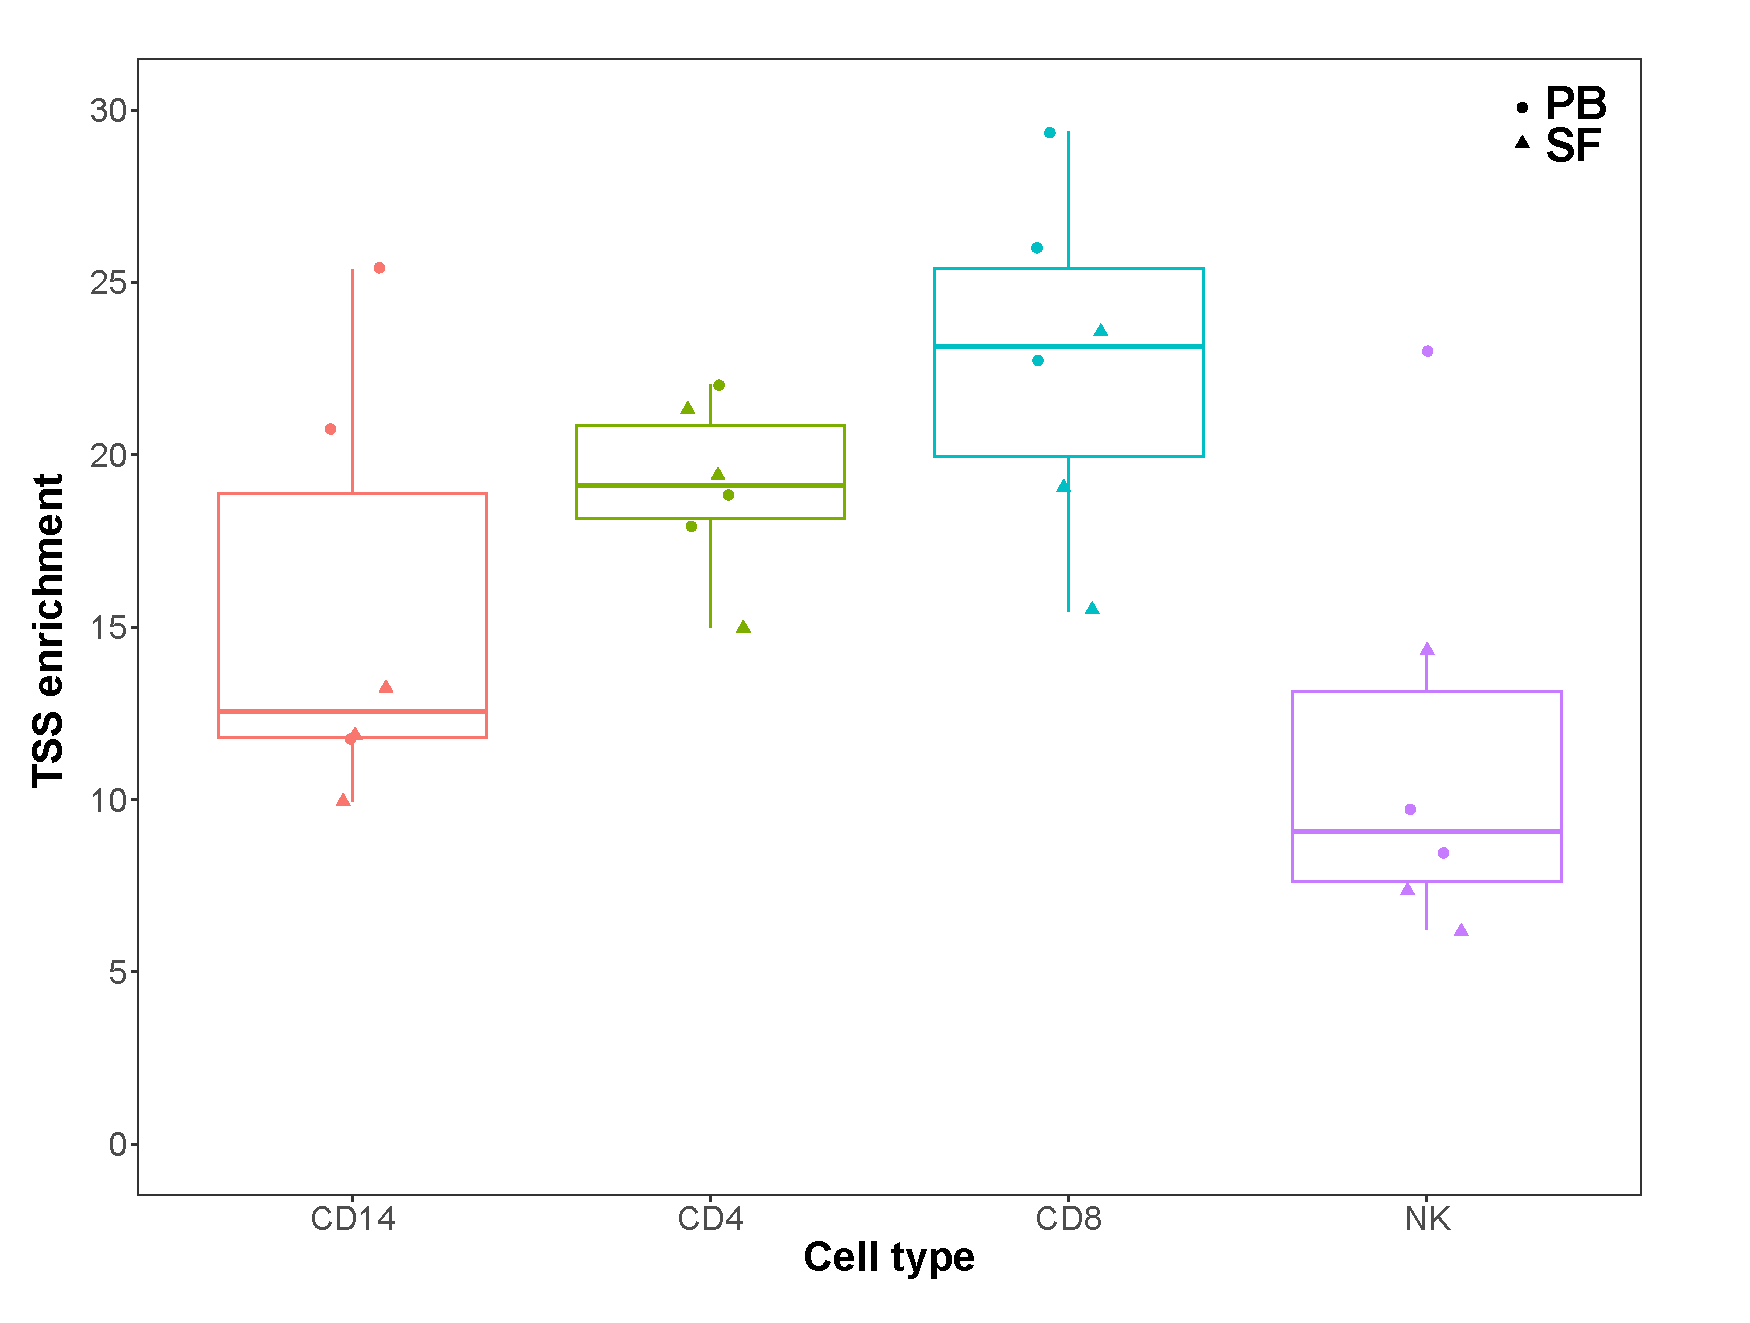
\includegraphics[width=\textwidth]{./Results3/pdfs/ATAC_PSA_all_TSS_max_per_cell_type}%
\caption{}
\end{subfigure}
\begin{subfigure}[b]{0.48\textwidth} 
%the [b] prevents offset in subcaptions
\centering
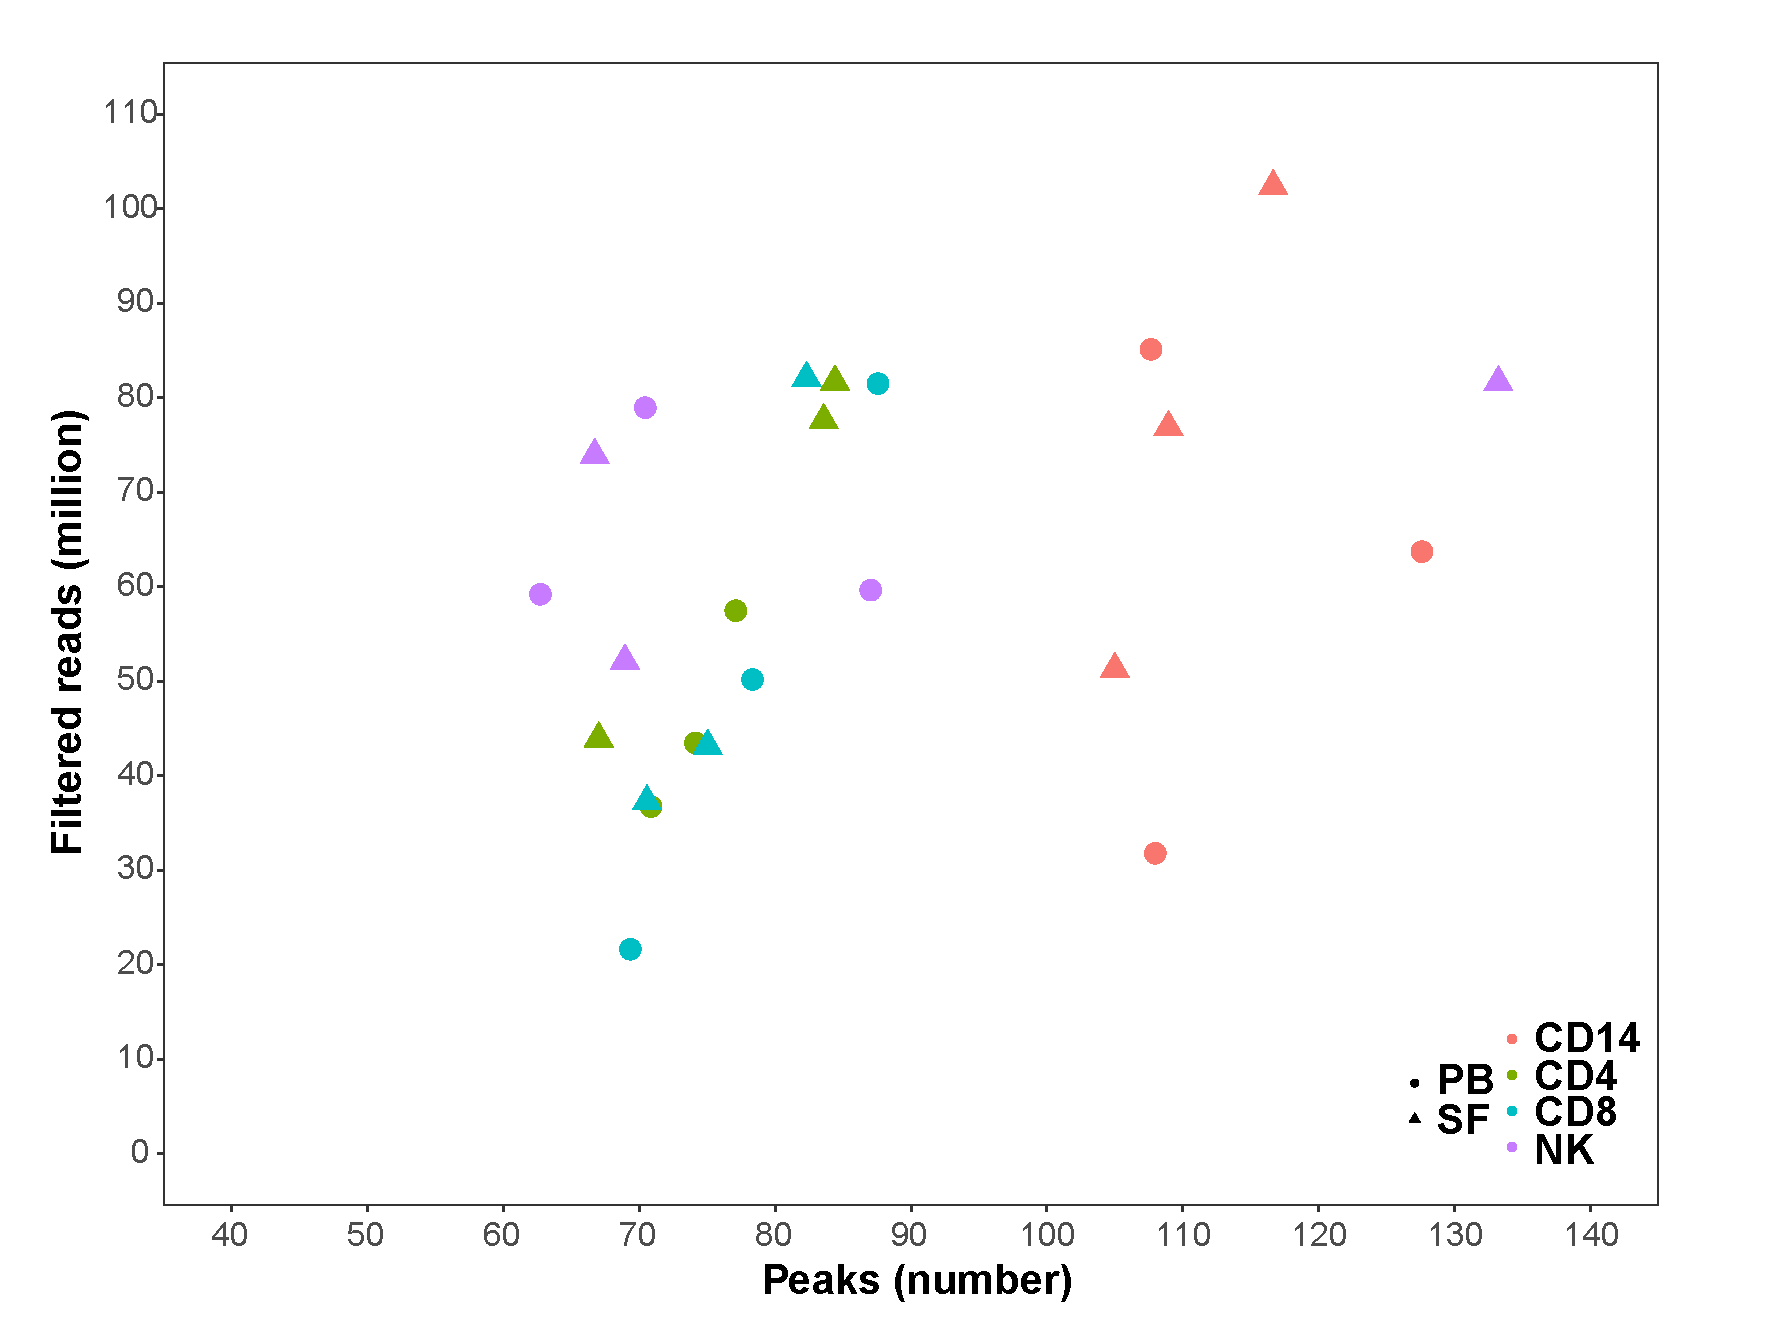
\includegraphics[width=\textwidth]{./Results3/pdfs/ATAC_PSA_all_peaks_vs_num_reads}%
\caption{}
\end{subfigure}
\caption[QC of FAST-ATAC PsA samples in four cell types]{\textbf{QC of FAST-ATAC PsA samples in four cell types}. }
\label{figure:PsA_FAST_ATAC_QC}
\end{figure}

When identifying open chromatin regions by peak calling using standard filtering (FDR$<$0.01), the number of accessible regions per sample ranged between $\sim$62$x10^3$ to $\sim$133$x10^3$ (Figure \ref{figure:PsA_FAST_ATAC_QC} d). A positive correlation between the number of called peaks and number of reads after filtering could be observed in the data. For example, CD14$^+$ was the cell type with greatest number of called peaks (108.4$x10^3$) as well as the greater median of reads remaining after filtering when compared to the other three cell types (Figure \ref{figure:PsA_FAST_ATAC_QC} a). Overall, appropriate number of peaks were called in all samples and no concerning outliers were identified.
%For example, the two NK samples with the greatest TSS enrichment (PSA1718 SF and PB) showed larger number of called peaks when compared to the other NK samples with similar number of reads but lower quality measured by TSS enrichment. This observation was consistent with the correlation between sample quality and the number of identified accessible chromatin regions previously demonstrated in Chapter \ref{ch:Results1}. 



\subsubsection{Accessible chromatin reflects cell type specificity and functional relevance}
To determine the ability of in house pipeline open chromatin to recapitulate cell type specificity in the PsA sample cohort, a combined master list including all four cell types and the two tissues was built. Following Chapter \ref{ch:Mat} and Chapter \ref{ch:Results1}, the combined master list contained open chromatin regions identified in at least 30\% of the samples (7 out of 24 samples), regardless cell type and tissue to avoid any bias. PCA analysis based on chromatin accessibility showed that most of the samples variability (PC1 65.6\% of the variability) correlated with cell type, leading to sample separation in four cluster (Figure \ref{figure:PsA_FAST_ATAC_PCA}). As expected, the myeloid (CD14$^+$ monocytes) and lymphoid (mCD4$^+$ and mCD8$^+$) clusters were the ones presenting greatest differences in chromatin accessibility pattern whereas the mCD4$^+$ and mCD8$^+$ clusters were the most similar between them. Modest clear separation between SF and PB samples was found in the mCD4$^+$, mCD8$^+$ and NK clusters.

\begin{figure}[H]
\centering
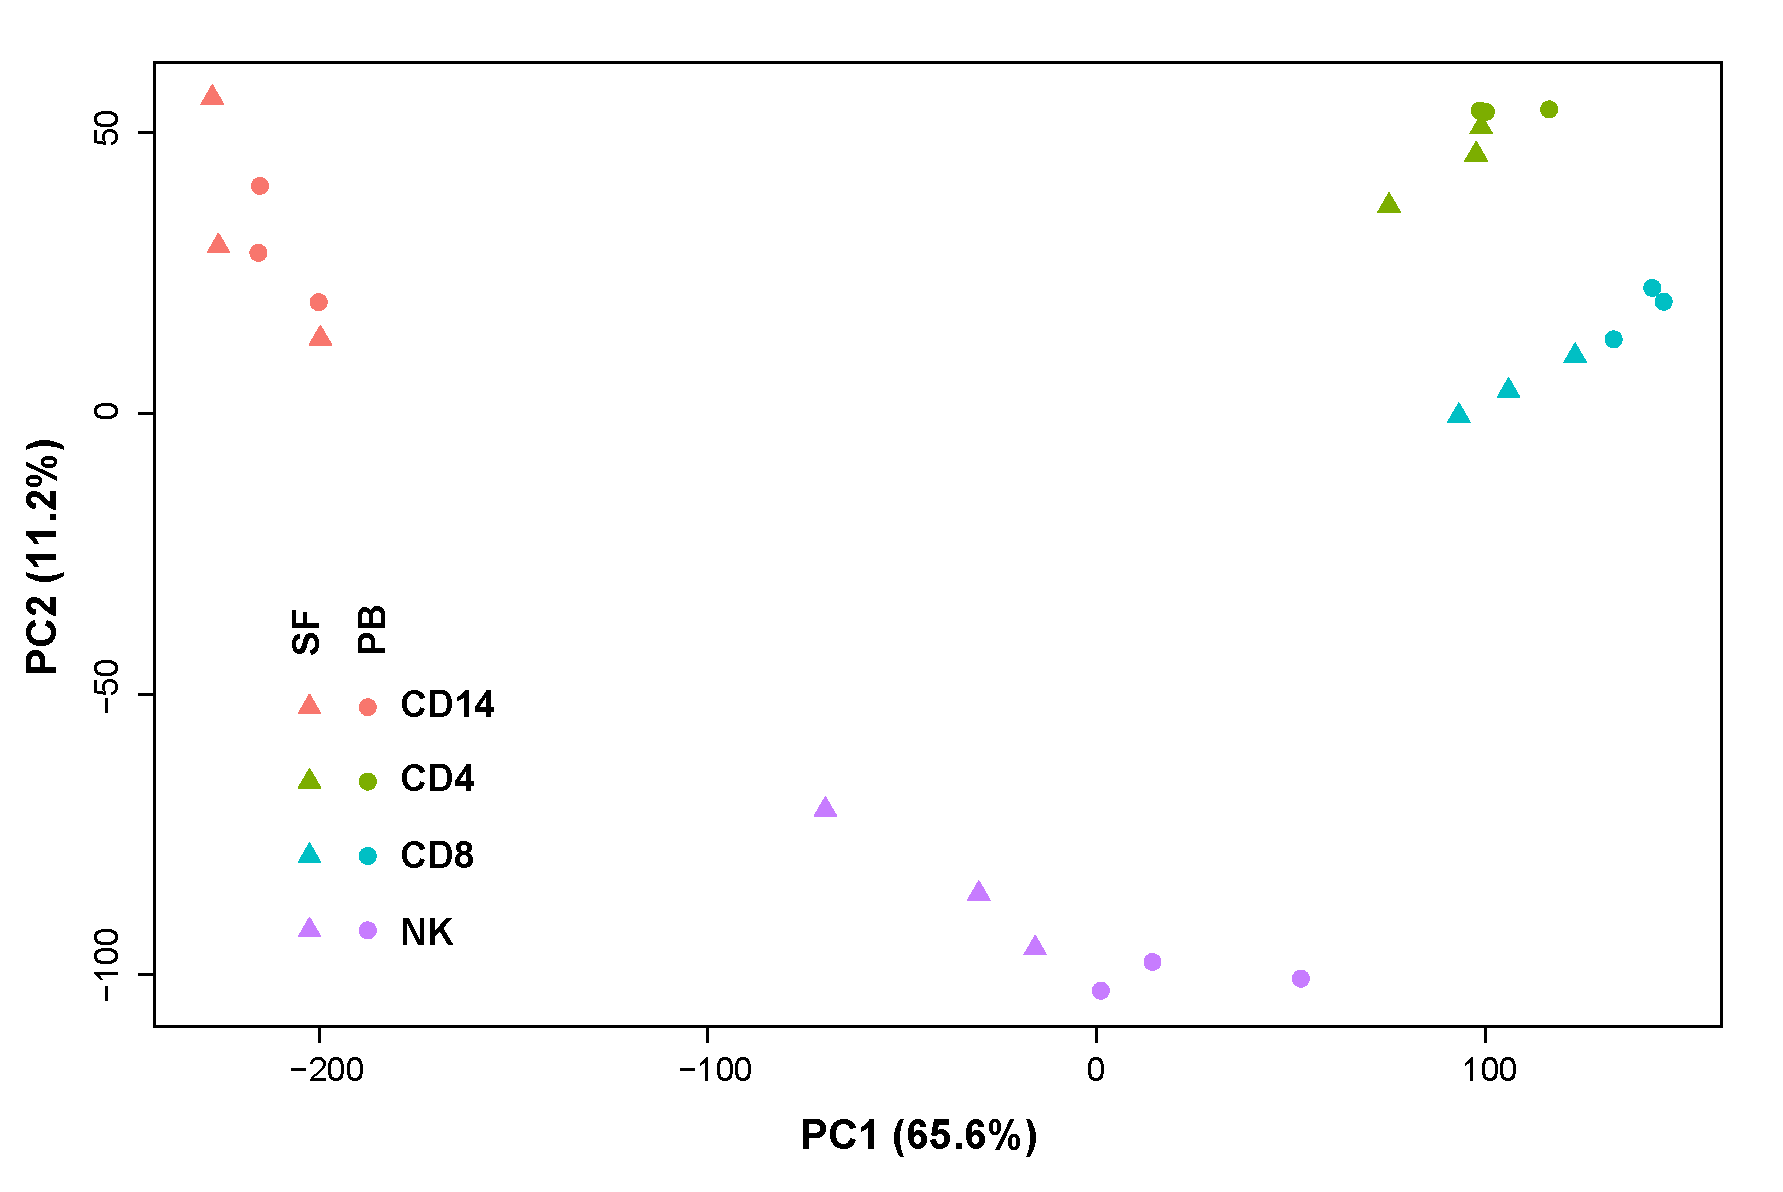
\includegraphics[width=0.7\textwidth]{./Results3/pdfs/ATAC_PSA_all_DESEq2_PCA}
\caption[Combined PCA analysis of all four cell types isolated from blood and SF.]{\textbf{Combined PCA analysis of all four cell types isolated from blood and SF.}}
\label{figure:PsA_FAST_ATAC_PCA}
\end{figure}

The ability to capture putative regulatory regions within the identified accessible chromatin in the four cell types was also explored. Enrichment analysis of different eQTL publicly available data sets for the combined chromatin accessibility master list was performed. Amongst the GTEx eQTL data, the greatest (z-score) and most significant (-log$_10$FDR) enrichment was found for the venous blood data set (red dot), consistently with the cell types included in the study (Figure \ref{figure:PsA_FAST_ATAC_eQTL_enrichment} a). Moreover, the greatest enrichments of immune-related cells in the accessible chromatin regions were found for CD14$^+$ monocytes (importantly unstimulated, LPS 2h and IFN-$\gamma$ 24h) followed by mCD8$^+$ T cells (Figure \ref{figure:PsA_FAST_ATAC_eQTL_enrichment} b). Interestingly, the B cells eQTLs were the least enriched in the chromatin accessibility data, consistently with the limited relevance of this cell type in psoriasis and PsA pathophysiology as well as the absence of this cell type amongst the ones included in the study.       

\bigskip
\begin{figure}[H]
\centering
\begin{subfigure}[b]{0.7\textwidth}
\centering 
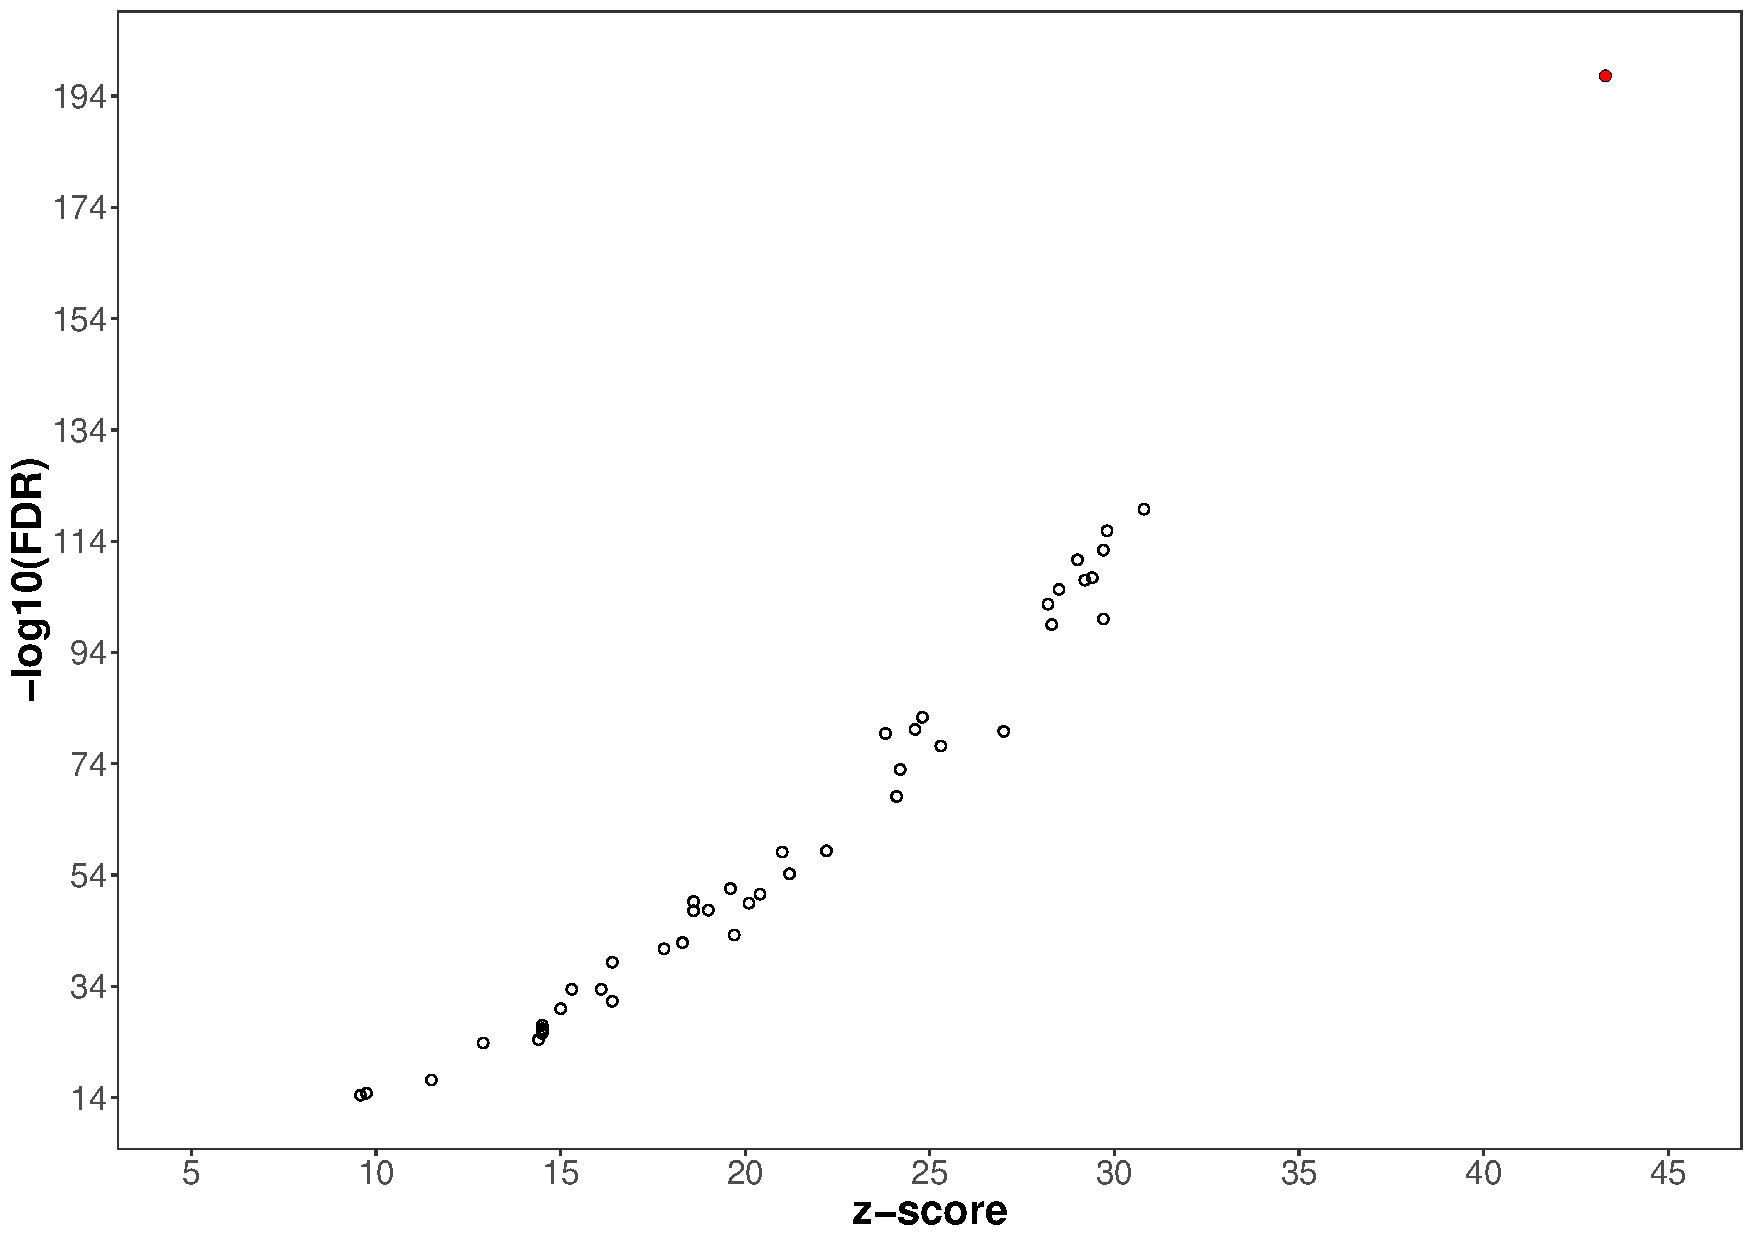
\includegraphics[width=\textwidth]{./Results3/pdfs/ATAC_PSA_all_GTeX_eQTL_enrichment_dotplot}
\caption{}
\end{subfigure}
~
\begin{subfigure}[b]{0.7\textwidth} 
%the [b] prevents offset in subcaptions
\centering
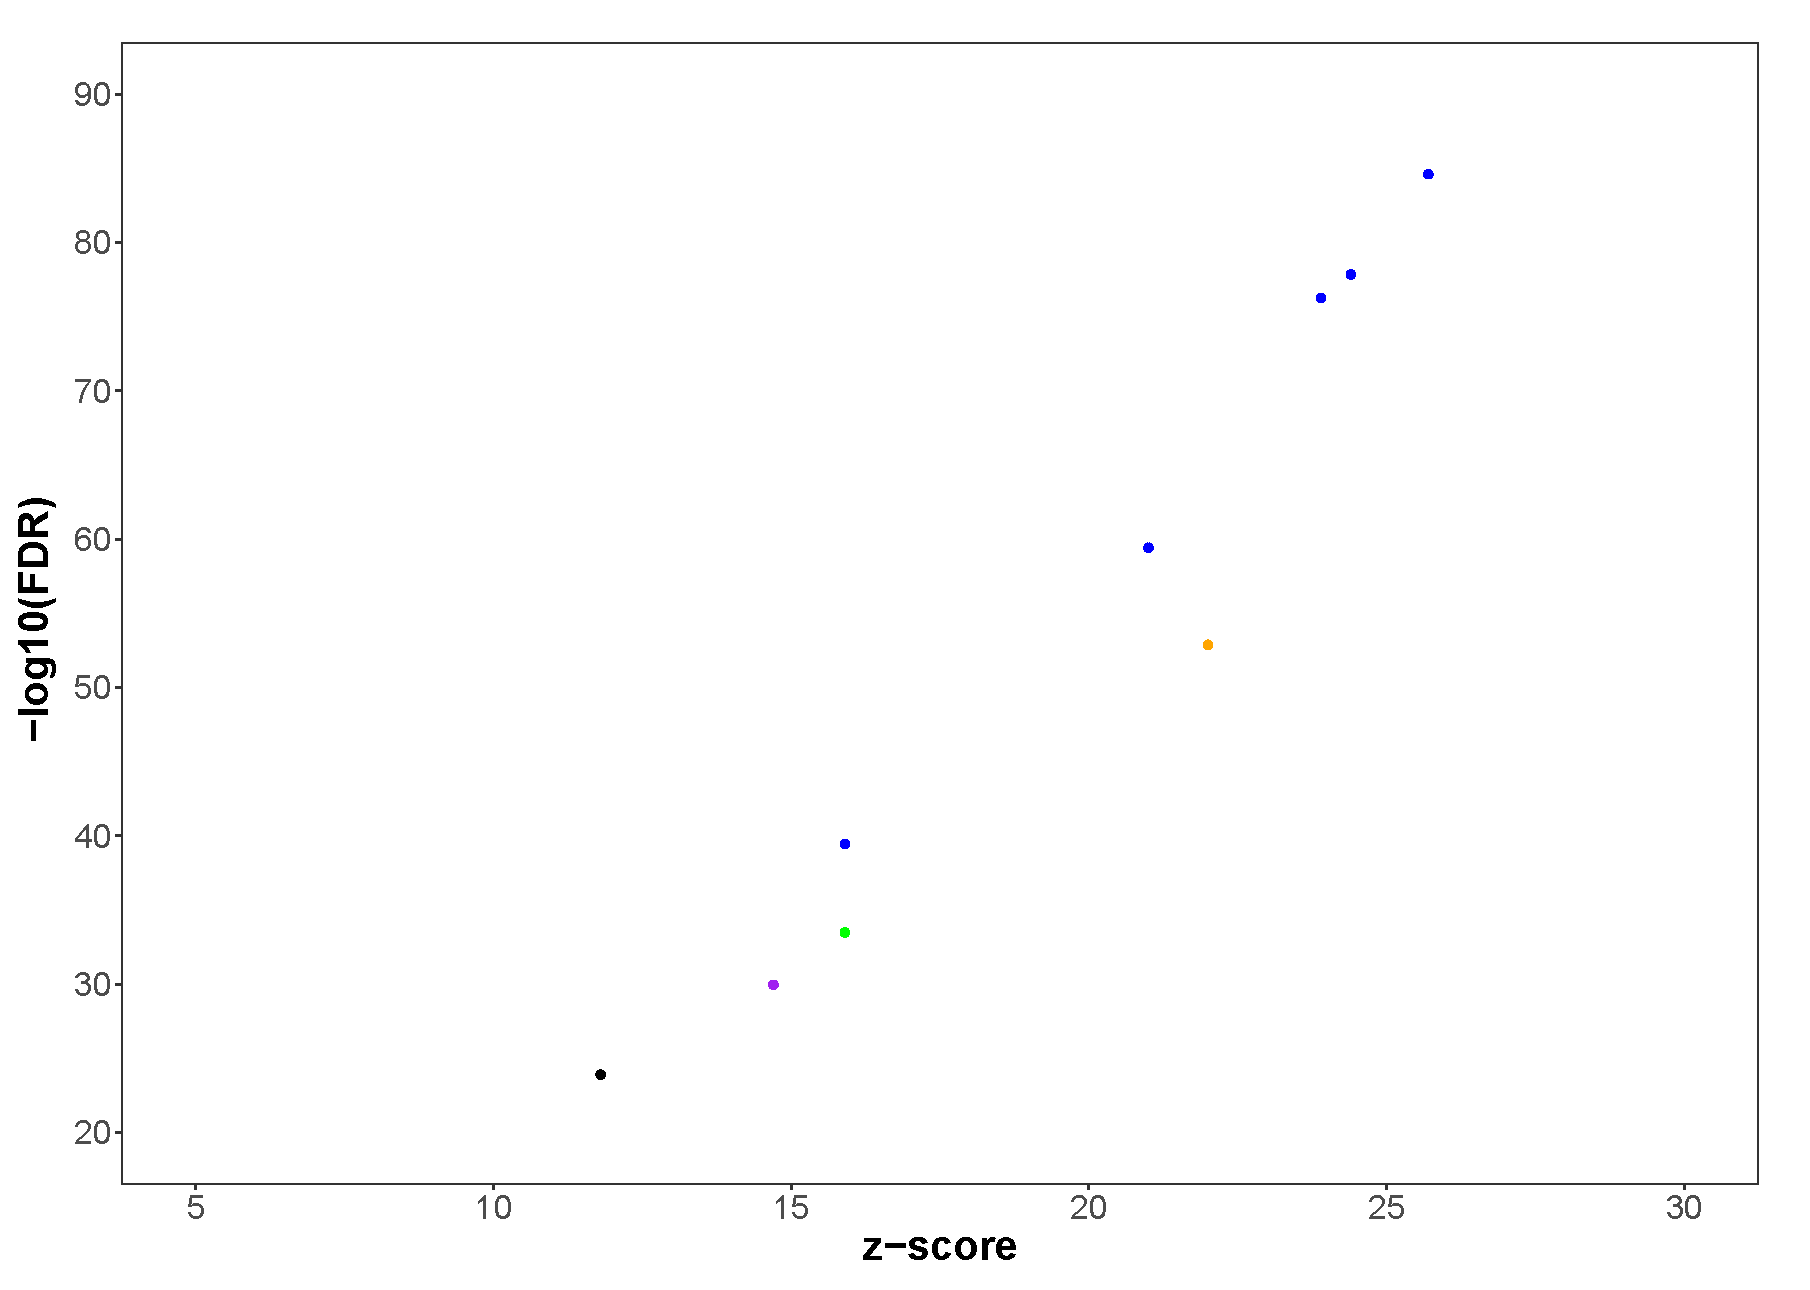
\includegraphics[width=\textwidth]{./Results3/pdfs/ATAC_PSA_all_Jknight_eQTL_enrichment_dotplot}
\caption{}
\end{subfigure}
\caption[Enrichment of eQTLs publicly available data in the combined cell type and tissue chromatin accessibility master list for the PsA cohort.]{\textbf{Enrichment of eQTLs publicly available data in the combined cell type and tissue chromatin accessibility master list for the PsA cohort.} The dot plots showed the z-score values of the enrichment analysis in the x-axis and the significance (-log$_10$FDR) in the y-axis for a) GTEx eQTL datasets and b) non-GTEx immune-related cell types including CD14$^+$ monocytes (unstimulated, 2 or 24h LPS stimulated and 24h IFN$\gamma$ stimulated) in blue, B-cells in black, total CD4$^+$ in green, total CD8$^+$ in orange and neutrophils in purple.}
\label{figure:PsA_FAST_ATAC_eQTL_enrichment}
\end{figure}





\subsubsection{Characterisation of the differential accessible chromatin regions}
Differential chromatin accessibility analysis was performed per cell type using a paired design between SF and PB for each of the four cell types (Table \ref{tab:PSA_DOCs_results}. For each of the cell types a master list containing chromatin accessible regions in at least 30\% of the samples ($\sim$2 samples), regardless the tissue. In all for analysis an 80\% cut-off for background noise was applied to the count matrix, as previously explained in Chapter 3. Only differentially open regions (DORs) identified with DESeq2 and also shared with quantile normalisation limma voom analysis where considered downstream. The CD14$^+$ monocytes and NK showed a greater proportion of DORs (23.3 and 8.9\%, respectively) compared to mCD4$^+$ and mCD8$^+$ T cells. In CD14$^+$ monocytes a significantly greater number of DORs more accessible  in SF (3,779 DORs) were found compared to PB (1,506 DORs). Conversely, the number of open DORs in Sf and PB were evenly distributed between in the other three cell types.


\begin{table}[htbp]
%\setlength{\tabcolsep}{20pt} only to stretch the columns if you want
%\renewcommand{\arraystretch}{1.5}
\centering
\begin{tabular}{@{}c c c c c}
\toprule
\textbf{Cell type}  & \textbf{Total DORs} &  \textbf{Proportion}  & \textbf{DORs open} & \textbf{DORs open} \\
                    &                     &  \textbf{DORs (\%)}  & \textbf{in SF} & \textbf{in PB} \\
\midrule
\midrule
CD14$^+$ & 5,285 & 23.3 & 3,779 & 1,506 \\
CD4$^+$  & 1,329 & 4.3 & 621 & 708 \\
CD8$^+$  & 1,570 & 4.5 & 807 & 763 \\
NK       & 2,314 & 8.9 & 1,223 & 1,091 \\
\bottomrule
\end{tabular}
\medskip %gap
\caption[Summary results of the chromatin accessibility analysis between SF and PB in PsA samples]{\textbf{Summary results of the chromatin accessibility analysis between SF and PB in PsA samples.}}
\label{tab:PSA_DOCs_results}
\end{table}

Permutation analysis using the ten unique possible combinations demonstrated that greater number of DORs than expected by chance were obtained in the differential analysis (Figure \ref{figure:PsA_perm_analysis}). This reinforced the fact that the identified changes in chromatin accessibility are driven by true differences between SF and PB in all the analysed cell types and therefore are specific.
  
When performing genomic annotation of the DORs in each of the cell types, intronic and intergenic regions consistently represented 80\% or more of all regions with differential accessibility (Figure \ref{figure:PsA_FAST_ATAC_DOCS_annotation} a). Universal promoter regions represented the third genomic feature with approximately between 5 to 15\% of the DORs annotation. In addition to this, the fifteen cell type-specific chromatin states from the Epigenome Roadmap segmentation maps were also used for annotation (Figure \ref{figure:PsA_FAST_ATAC_DOCS_annotation} b). For all four cell types DORs, between 44.96 and 72.11\% were annotated as weak enhancers, which represented the most prominent category and the most significantly enriched (data not shown). This was consistent with the predominance of introns and intergenic regions, as those are the preferred location for enhancer elements. Although modest percentages of heterochromatin and repetitive regions were observed, enrichment was not significant for these two chromatin states in any of the four cell types (data not shown).
%

\bigskip
\begin{figure}[H]
\centering
\begin{subfigure}[b]{0.7\textwidth}
\centering 
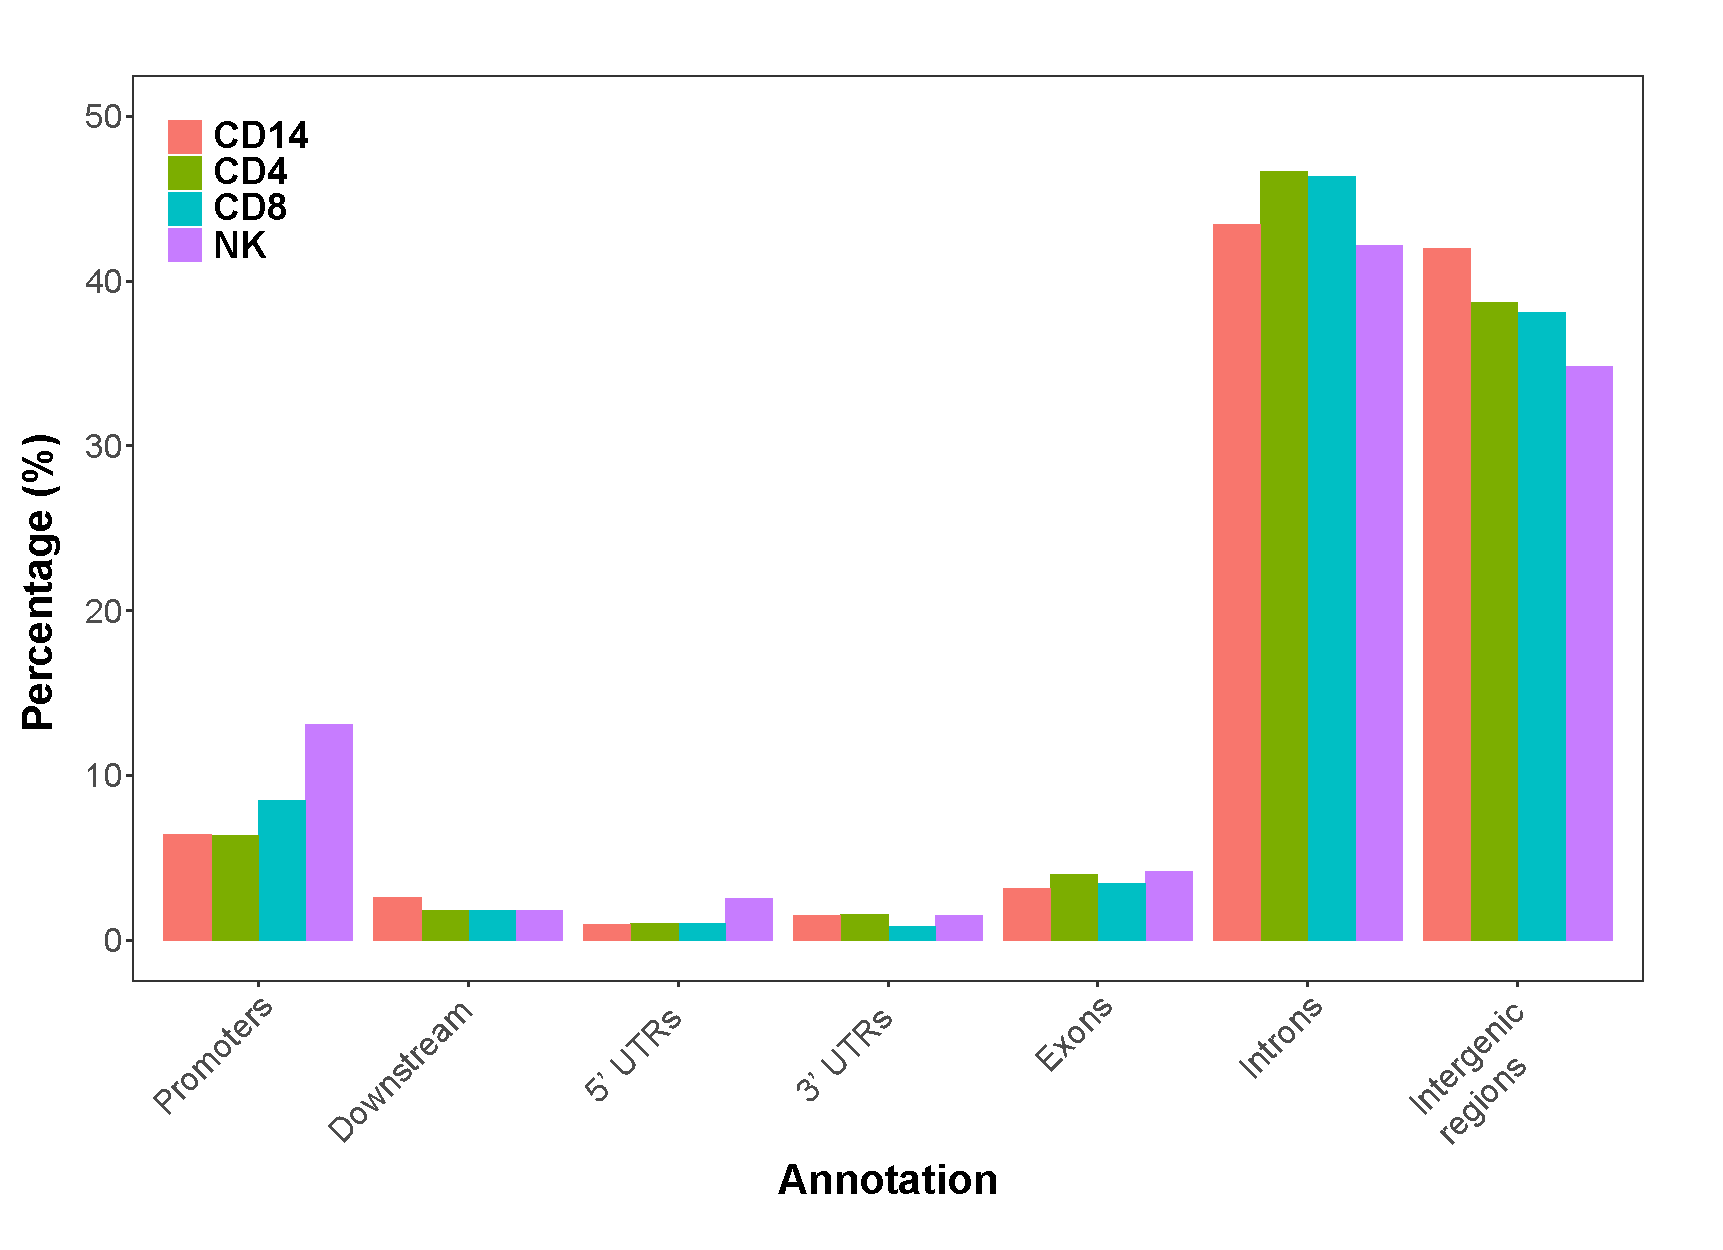
\includegraphics[width=\textwidth]{./Results3/pdfs/ATAC_PSA_DOCS_per_cell_type_general_annotation}
\caption{}
\end{subfigure}
~
\begin{subfigure}[b]{0.7\textwidth} 
%the [b] prevents offset in subcaptions
\centering
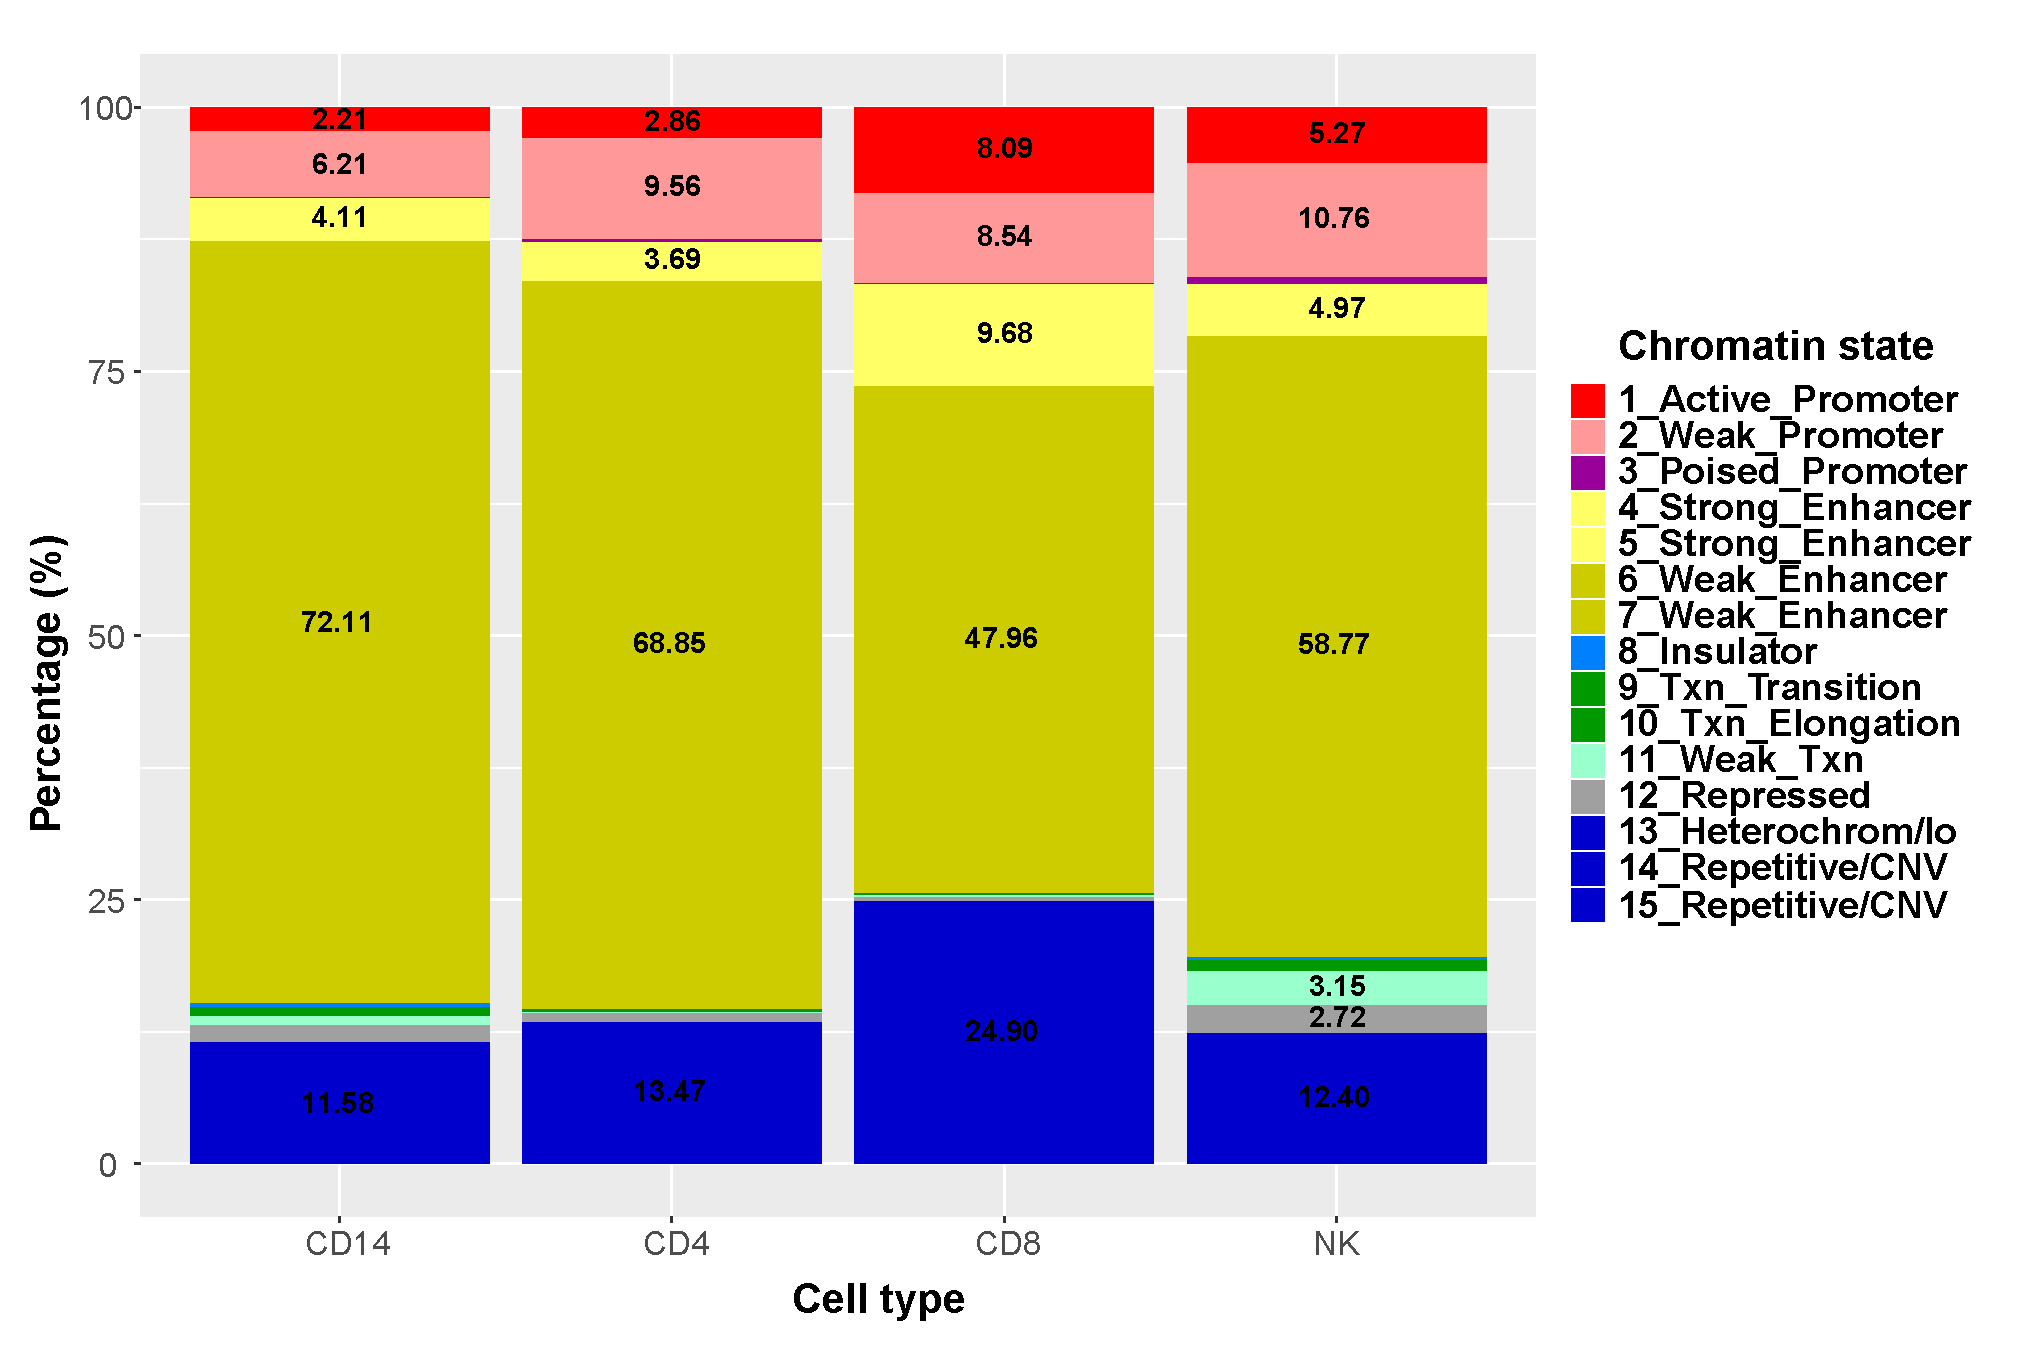
\includegraphics[width=\textwidth]{./Results3/pdfs/ATAC_PSA_DOCS_chromatin_states_stacked_barplot}
\caption{}
\end{subfigure}
\caption[Annotation with genomic regions and chromatin states of the PsA DOCs from the four cell types differential analysis.]{\textbf{Annotation with genomic regions and chromatin states of the PsA DOCs from the four cell types differential analysis.} xxxx}
\label{figure:PsA_FAST_ATAC_DOCS_annotation}
\end{figure}


%Try to overlap the enhancer FANTOM data to id those regions whith evidence of eRNA expression
The functional relevance of the differential chromatin accessibility in terms of regulation of gene expression was further investigated by integration of the eRNA data from the FANTOM5 project. Statistically significant enrichment for robust and permissive enhancers was found for the DORs identified in the four cell types (Figure \ref{figure:PSA_FANTOM}). Robust enhancers are those for which transcription was significantly detected at the genome-wide level in at least one primary cell type or tissue, whereas the permissive set included also those not passing the filtering criteria \parencite{Andersson2014}. Moreover, DORs from all four cell types also presented significant enrichment for the corresponding cell type eRNA set amongst the top two most enriched. The proportion of DORs overlapping the appropriate cell type set of expressed eRNAs ranged between 19.8\% (83 open in SF and 160 open in PB) in NK and 31.8\% (83 open in SF and 160 open in PB) in CD4$^+$.


\begin{figure}[htbp]
\centering
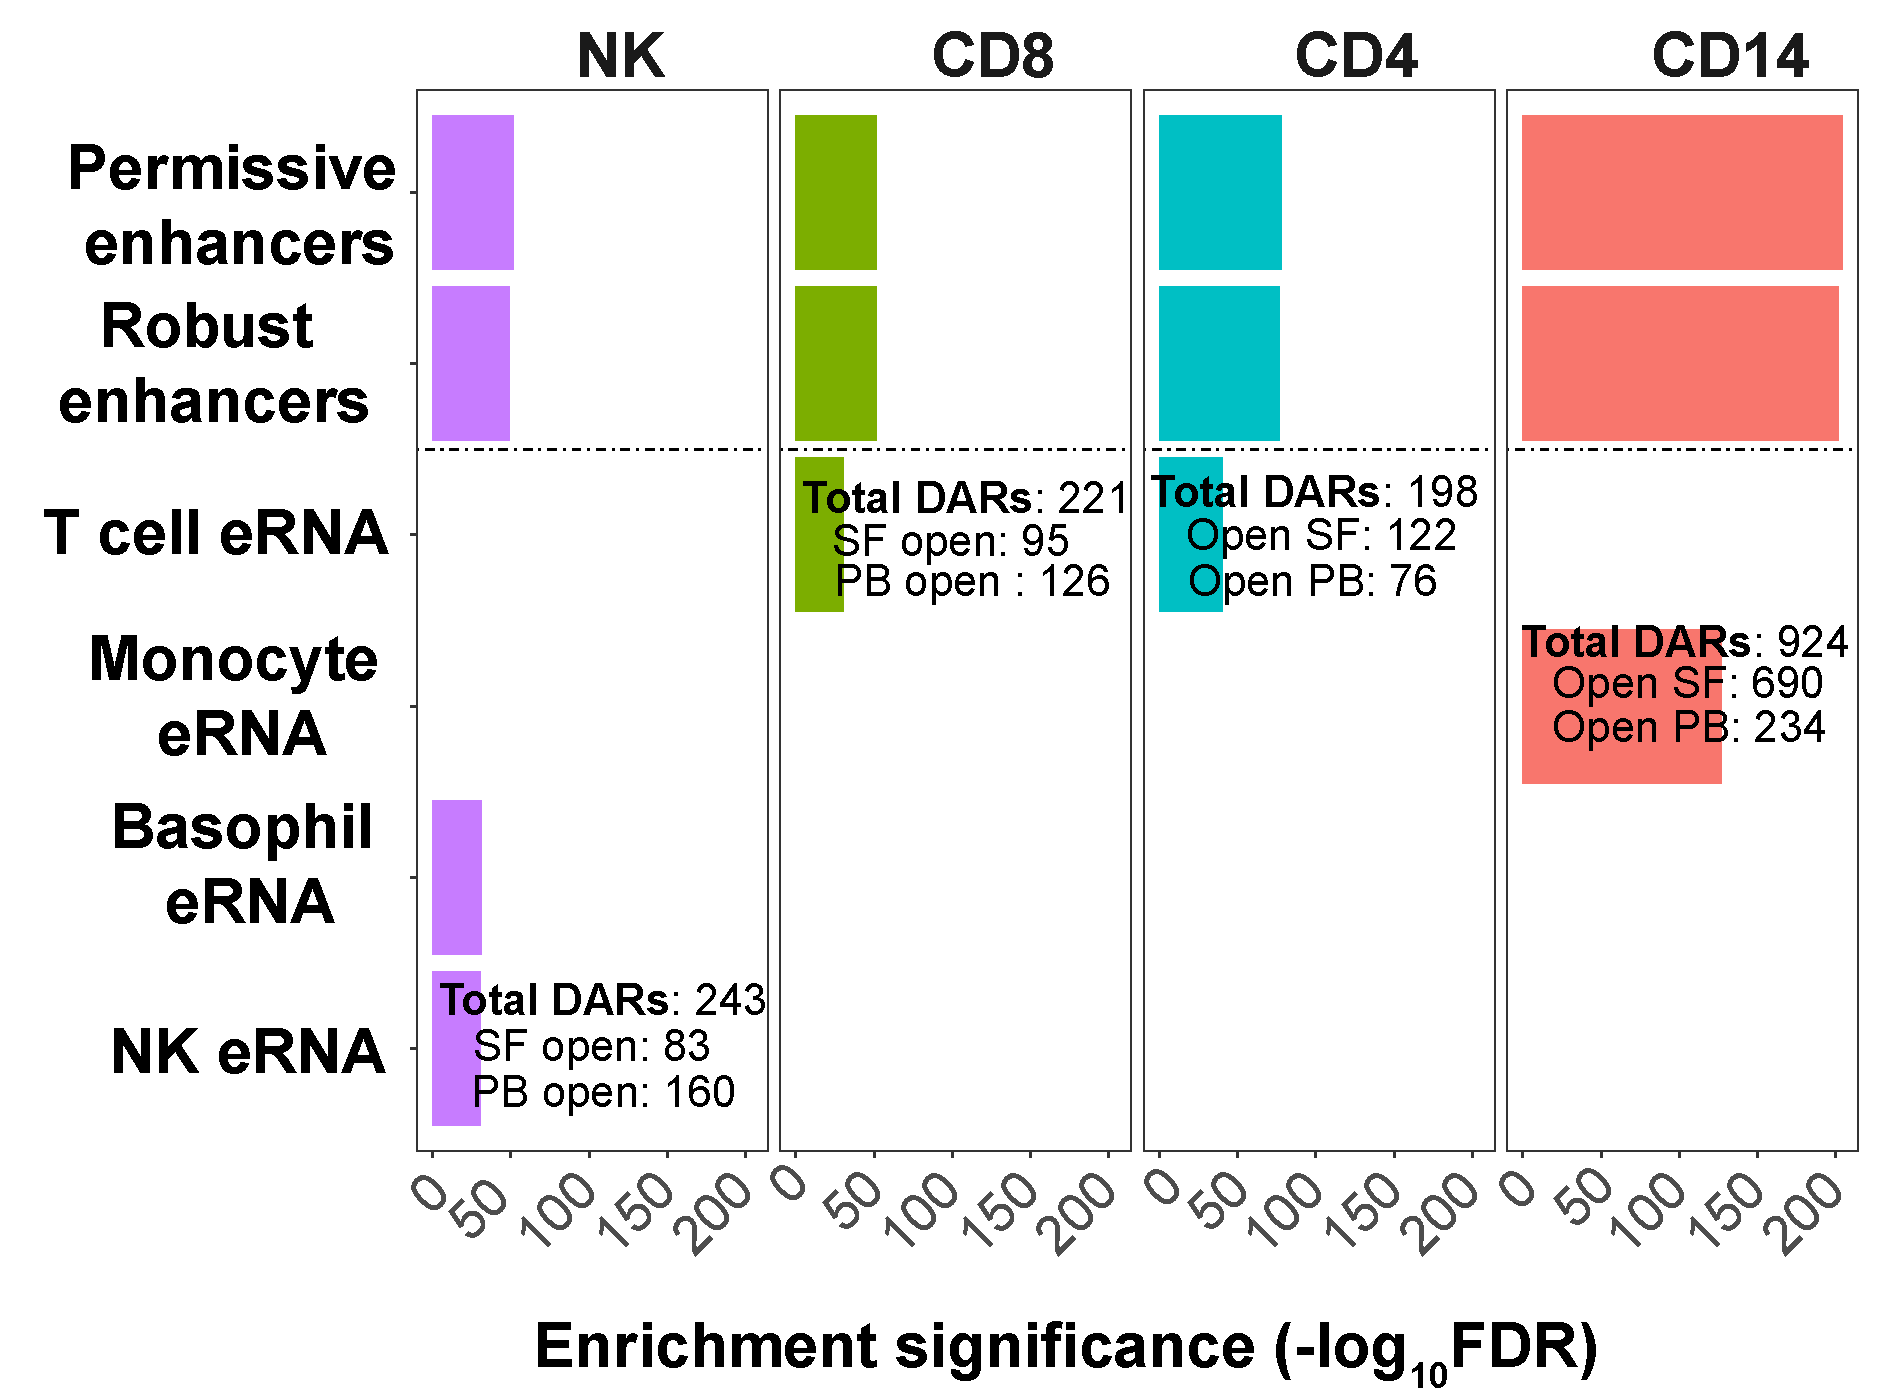
\includegraphics[width=0.8\textwidth]{./Results3/pdfs/ATAC_PsA_FANTOM_enhancer_enrichment_all_cell_types}
\caption[Enrichment of PsA DORs for the FANTOM5 eRNA dataset.]{\textbf{Enrichment of PsA DOCs for the FANTOM5 eRNA dataset.} xxx }
\label{fig:PSA_FANTOM}
\end{figure}

From the differential analysis between SF and PB in all four cell types, a number of DORs were overlapping a gene body (Table \ref{tab:PSA_DOCs_gene_body}). Interestingly, the majority were located within introns instead of untranslated regions (UTRs) and have also been annotated as weak or strong enhancers according to the cell type specific chromatin segmentation map. 

%Similarly, more accessible chromatin in SF compared to PB was identified in five regions of the \textit{IL15} gene, annotated as promoter and enhancers in CD14$^+$ monocytes. 
% Check differences at both gene locations were CD14$^+$ cell type specific is this region HiC annotated with the gene? and maybe include example overlapping eRNA
%e.g LMNA4 which is CD14 cell specific and more expressed in SF in Dolcino paper. Maybe use it later

\begin{table}[htbp]
%\setlength{\tabcolsep}{20pt} only to stretch the columns if you want
%\renewcommand{\arraystretch}{1.5}
\centering
\begin{tabular}{@{} c c c c c}
\toprule
\textbf{Cell type} & \textbf{DORs in gene body} &  \textbf{Gene with $>$ one DOR} &\textbf{Enhancers} & \textbf{Introns} \\
\midrule
\midrule
CD14$^+$ & 2,357 & 744 & 1,775 & 1,920 \\
CD4$^+$ & 700 & 99 & 504 & 577 \\
CD8$^+$ & 831 & 118 & 503 & 666 \\
NK   & 1,246 & 235 & 782 & 937 \\   
\bottomrule
\end{tabular}
\medskip %gap
\caption[Annotation of gene body DORs in four cell types from PsA samples.]{\textbf{Annotation of gene body DORs in four cell types from PsA samples.}xxxx}
\label{tab:PSA_DOCs_gene_body}
\end{table}

As an example, a more accessible PB DOR located in an intron of the \textit{VAV3} gene and significantly expressed as eRNA was identified in NK (Figure \ref{figure:PsA_FAST_ATAC_gene_boy_DOCS_CD14_NK} a). Additionally, for all four cell types, a number of gene entities contained more than one DOR, showing the same direction of chromatin accessibility between SF and PB. For example, in CD14$^+$ two DORs located at the 5' and 3' UTRs for \tetxit{IL7R} gene where found to be more accessible in SF compared to PB (Figure \ref{figure:PsA_FAST_ATAC_gene_boy_DOCS_CD14_NK} b). 

\bigskip
\begin{figure}[H]
\centering
\begin{subfigure}[b]{0.70\textwidth}
\centering 
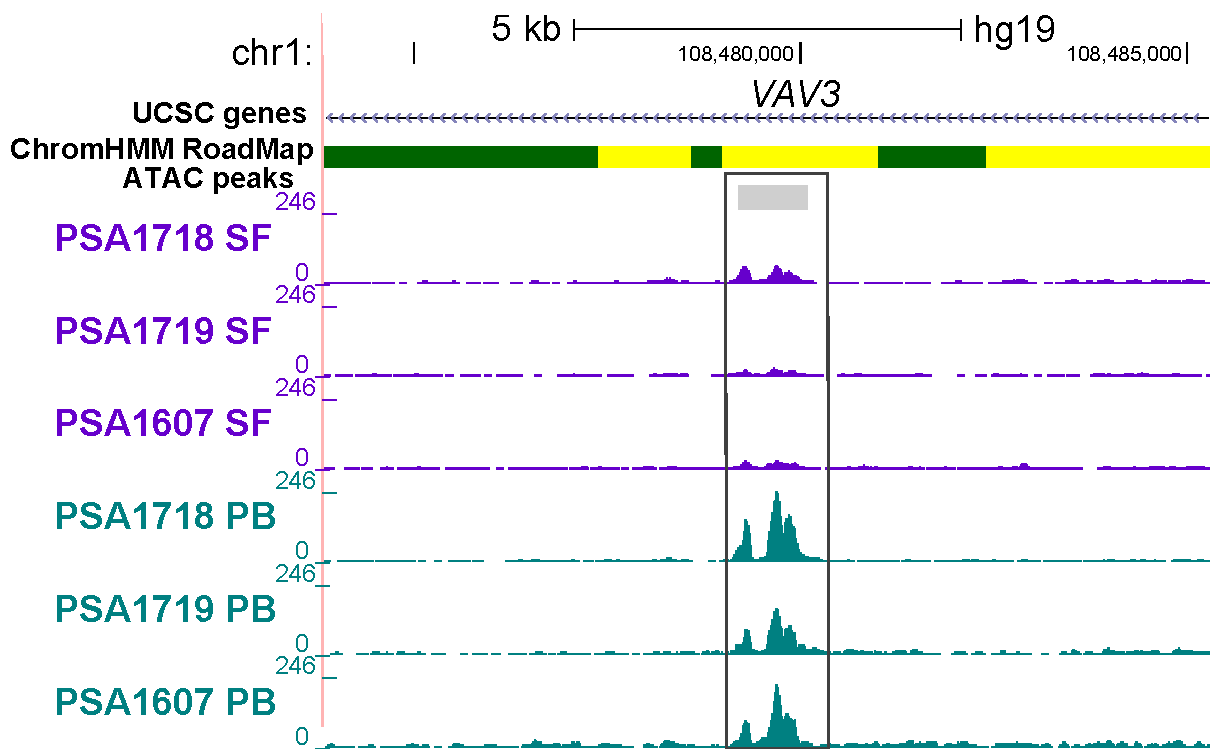
\includegraphics[width=\textwidth]{./Results3/pdfs/ATAC_PSA_NK_VAV3}
\caption{}
\end{subfigure}
~
\begin{subfigure}[b]{0.70\textwidth} 
%the [b] prevents offset in subcaptions
\centering
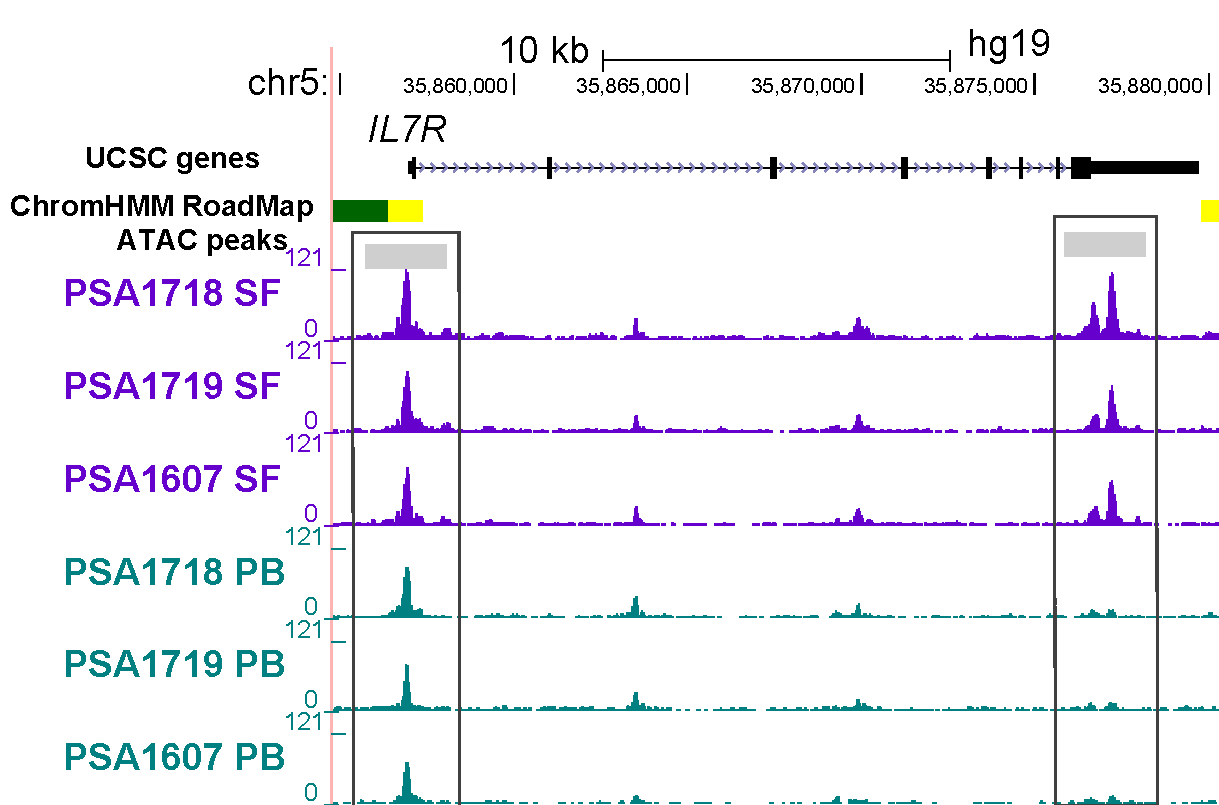
\includegraphics[width=\textwidth]{./Results3/pdfs/ATAC_PSA_CD14_IL7R}
\caption{}
\end{subfigure}
\caption[Differentially accessible regions located within gene bodies in CD14$^+$ monocytes and NK cells from PsA patients.]{\textbf{Differentially accessible regions located within gene bodies in CD14$^+$ monocytes and NK cells from PsA patients.} xxxx}
\label{figure:PsA_FAST_ATAC_gene_boy_DOCS_CD14_NK}
\end{figure}

% GWAS overlap maybe indicate an example in CD14 that can be relevant with pathway analysis
The relevance of the differences in chromatin accessibility in the context of psoriasis and PsA GWAS hits was also addressed. Enrichment analysis of psoriasis and PsA GWAS hits for the DORs in each of the four cell types was performed using XGR co-localisation and permutation analysis. At the SNP level, no significant enrichment was reported  between DORs and GWAS lead SNPs and those in LD r$^2$$\geq$8. However, significant enrichment (2-fold enrichment and empirical p-val 0.043) of the psoriasis and PsA GWAS LD blocks was observed only for the CD14$^+$ DORs.
%
%

\subsection{Pathway and TFBS enrichment analysis highlight tissue-specific functional differences in chromatin accessibility}

For each of the four sets of DORs, pathway enrichment analysis was conducted separately for those regions more accessible in SF and PB. Gene annotation of the DORs was performed by physical proximity, as detailed in Chapter \ref{ch:Mat}. Despite commonalities, differences in significant enriched pathways (FDR$<$0.01 or 0.05) were identified within the same cell type between SF and PB (Figure \ref{figure:PSA_ATAC_pathway_analysis_all_DOC}). In CD14$^+$ monocytes open chromatin in SF presented enrichment for pathways involved in regulation of immunity, inflammation and cell survival such as the NF-$\kapa$B pathway or cytokine production, including IL-2 signalling and IL-3, 5 and granulocyte-macrophage colony–stimulating factor (GM-CSF) pathways (Figure \ref{figure:PSA_ATAC_pathway_analysis_all_DOC} a). mCD4$^+$ DORs more open in SF compared to PB showed enrichment for T cell receptor signaling as well as chemokine signaling, which included DORs in proximity to IFN-$\gamma$, IL-2 receptor alpha (\textit{IL2RA}) and IL-5 receptor alpha (\textit{IL5RA}), amongst others (Figure \ref{figure:PSA_ATAC_pathway_analysis_all_DOC} b). This is consistent with the IL-2, IL-3 and IL-5pathway enrichment in open CD14$^+$ SF DORs. Although T cell signaling pathway appears only enriched for open SF DORS in mCD4$^+$, PB open regions in this cell type were enriched for focal adhesion members, also involved in the TCR signaling \parencite{XY}. Enriched pathways for open mCD8$^+$ were only significant when using an FDR$<0.5$ threshold. (Figure \ref{figure:PSA_ATAC_pathway_analysis_all_DOC} c). Interestingly, G protein coupled receptor (GPCR) signalling was enriched for mCD8$^+$ open PB DORs, consistently with the role of this pathway in chemotaxis. mCD8$^+$ DORs open in SF also showed enrichment for the Wnt signaling pathway involved in the production of memory cells with enhanced proliferative potential and stronger protective capacity. 


NK DORs open in SF presented enrichment for Fc-gamma receptor(FC$\gamma$R)-mediated phagocytosis that could be triggered by occurrence of monoclonal gammopathy of undetermined significance (MGUS) in PsA patients and consequently induce NK activation (Figure \ref{figure:PSA_ATAC_pathway_analysis_all_DOC} d). Moreover, members of the HIF-1 pathway were also enriched in NK open SF DORs, as hypoxic environment is induced in joint inflammation. Interestingly, enrichment of PB open DORs in the proximity of NK cell mediated toxicity genes was unveiled. According to FACS analysis, the proportion of NK CD56$\textsuperscript{bright}$ was greater in PB compared to SF in this sample cohort. This is consistent with the observed enrichment for NK cytotoxicity, since previous studies have demonstrated that CD56$\textsuperscript{bright}$ NK cells are preferentially cytokine producers than the cytotoxic active than the tissue resident ones. 
% NK CD56 bright subsets and tissue http://www.jimmunol.org/content/196/7/2923.long
% Production of IgG in PsA http://www.jrheum.org/content/41/12/2421.long
% NK phagocytisis FCgamma R III https://www.ncbi.nlm.nih.gov/pmc/articles/PMC1550276/, https://www.sciencedirect.com/science/article/pii/S0022202X15300373#bb0030, https://www.sciencedirect.com/science/article/pii/S0022202X15300373#bb0185
%Joint hypoxia https://www.ncbi.nlm.nih.gov/pmc/articles/PMC3683428/
%Skin hypoxia https://www.sciencedirect.com/science/article/pii/S0022202X15331328?via%3Dihub

\begin{figure}[H]
\centering
\begin{subfigure}[b]{0.45\textwidth}
\centering 
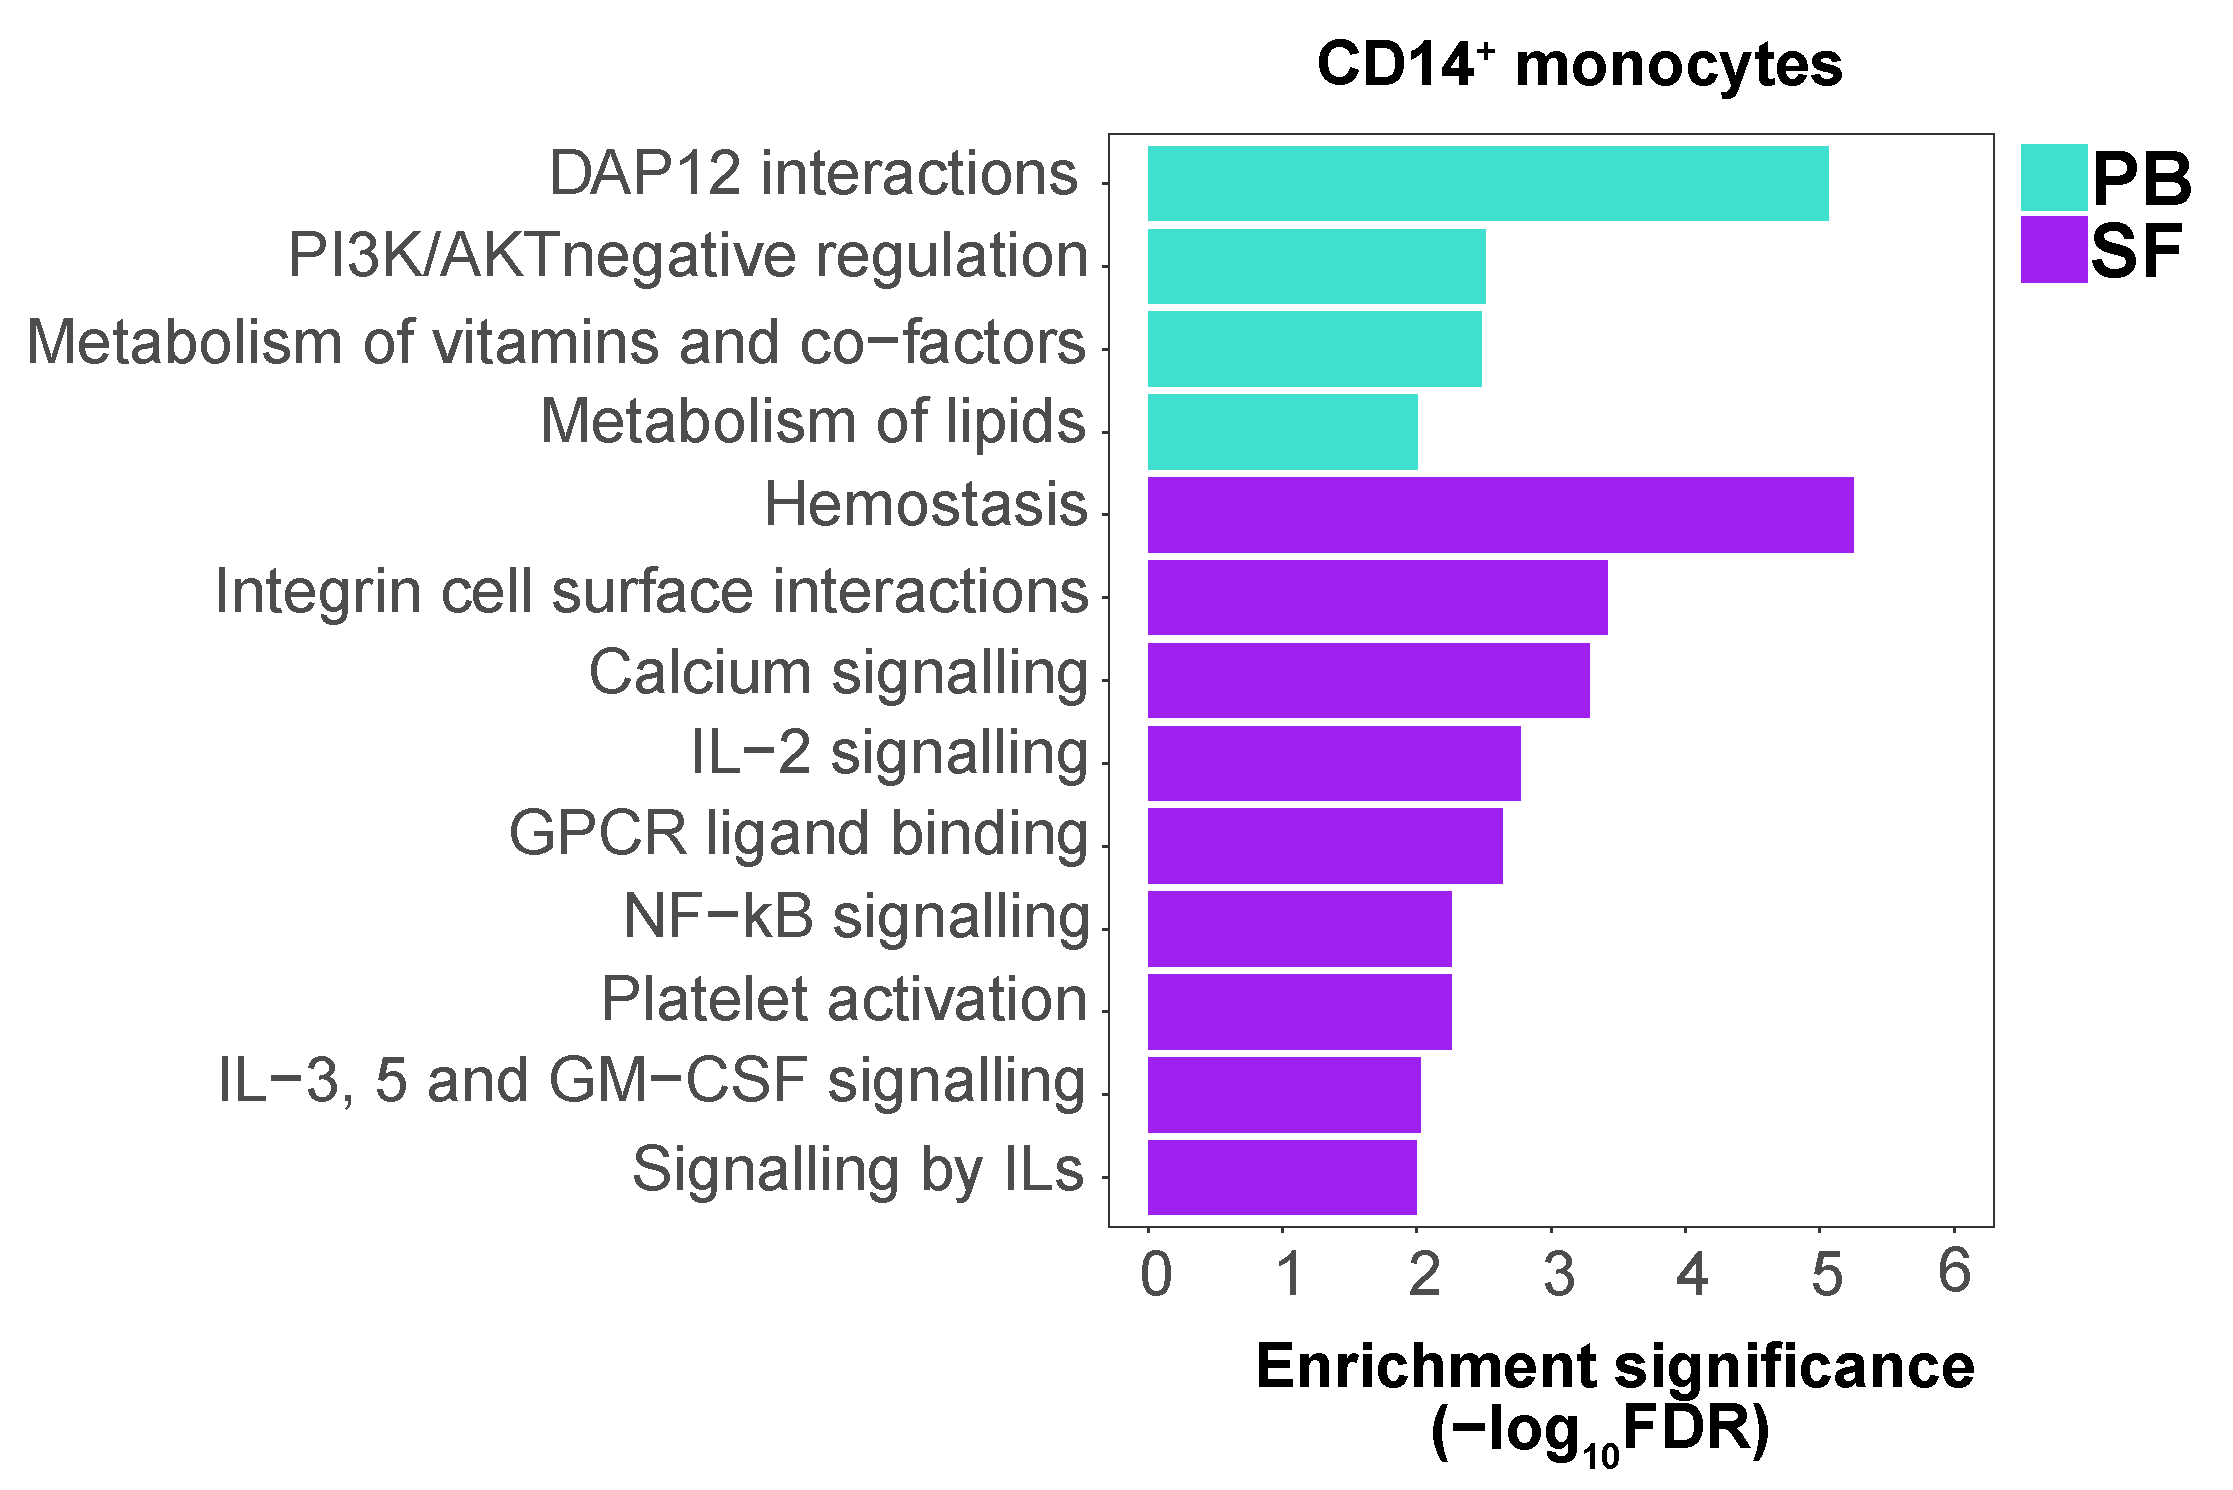
\includegraphics[width=\textwidth]{./Results3/pdfs/ATAC_PSA_CD14_pathways_barplot_all_DOCS_proximity}
\caption{}
\end{subfigure}
~
\begin{subfigure}[b]{0.45\textwidth}
\centering 
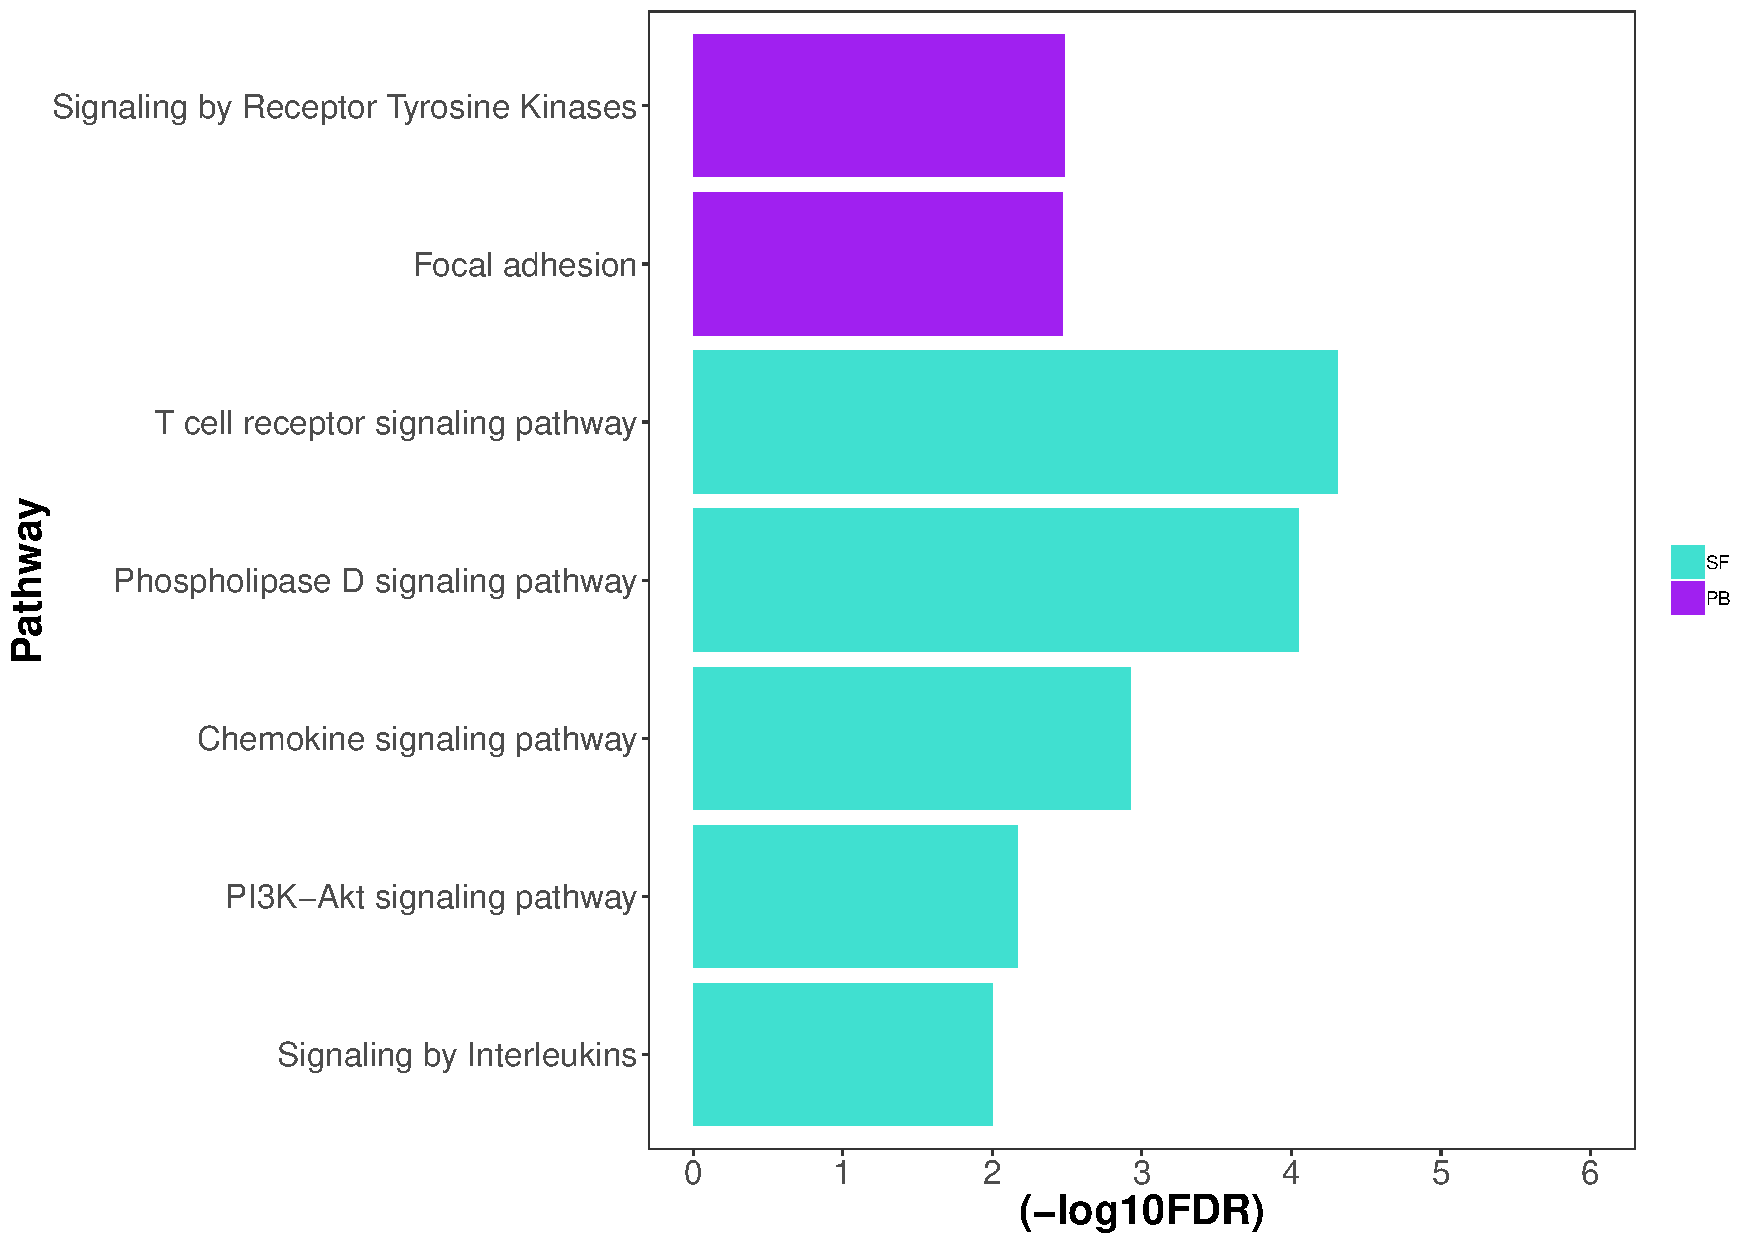
\includegraphics[width=\textwidth]{./Results3/pdfs/ATAC_PSA_CD4_pathways_barplot_all_DOCS_proximity}
\caption{}
\end{subfigure}
~
\begin{subfigure}[b]{0.45\textwidth} 
%the [b] prevents offset in subcaptions
\centering
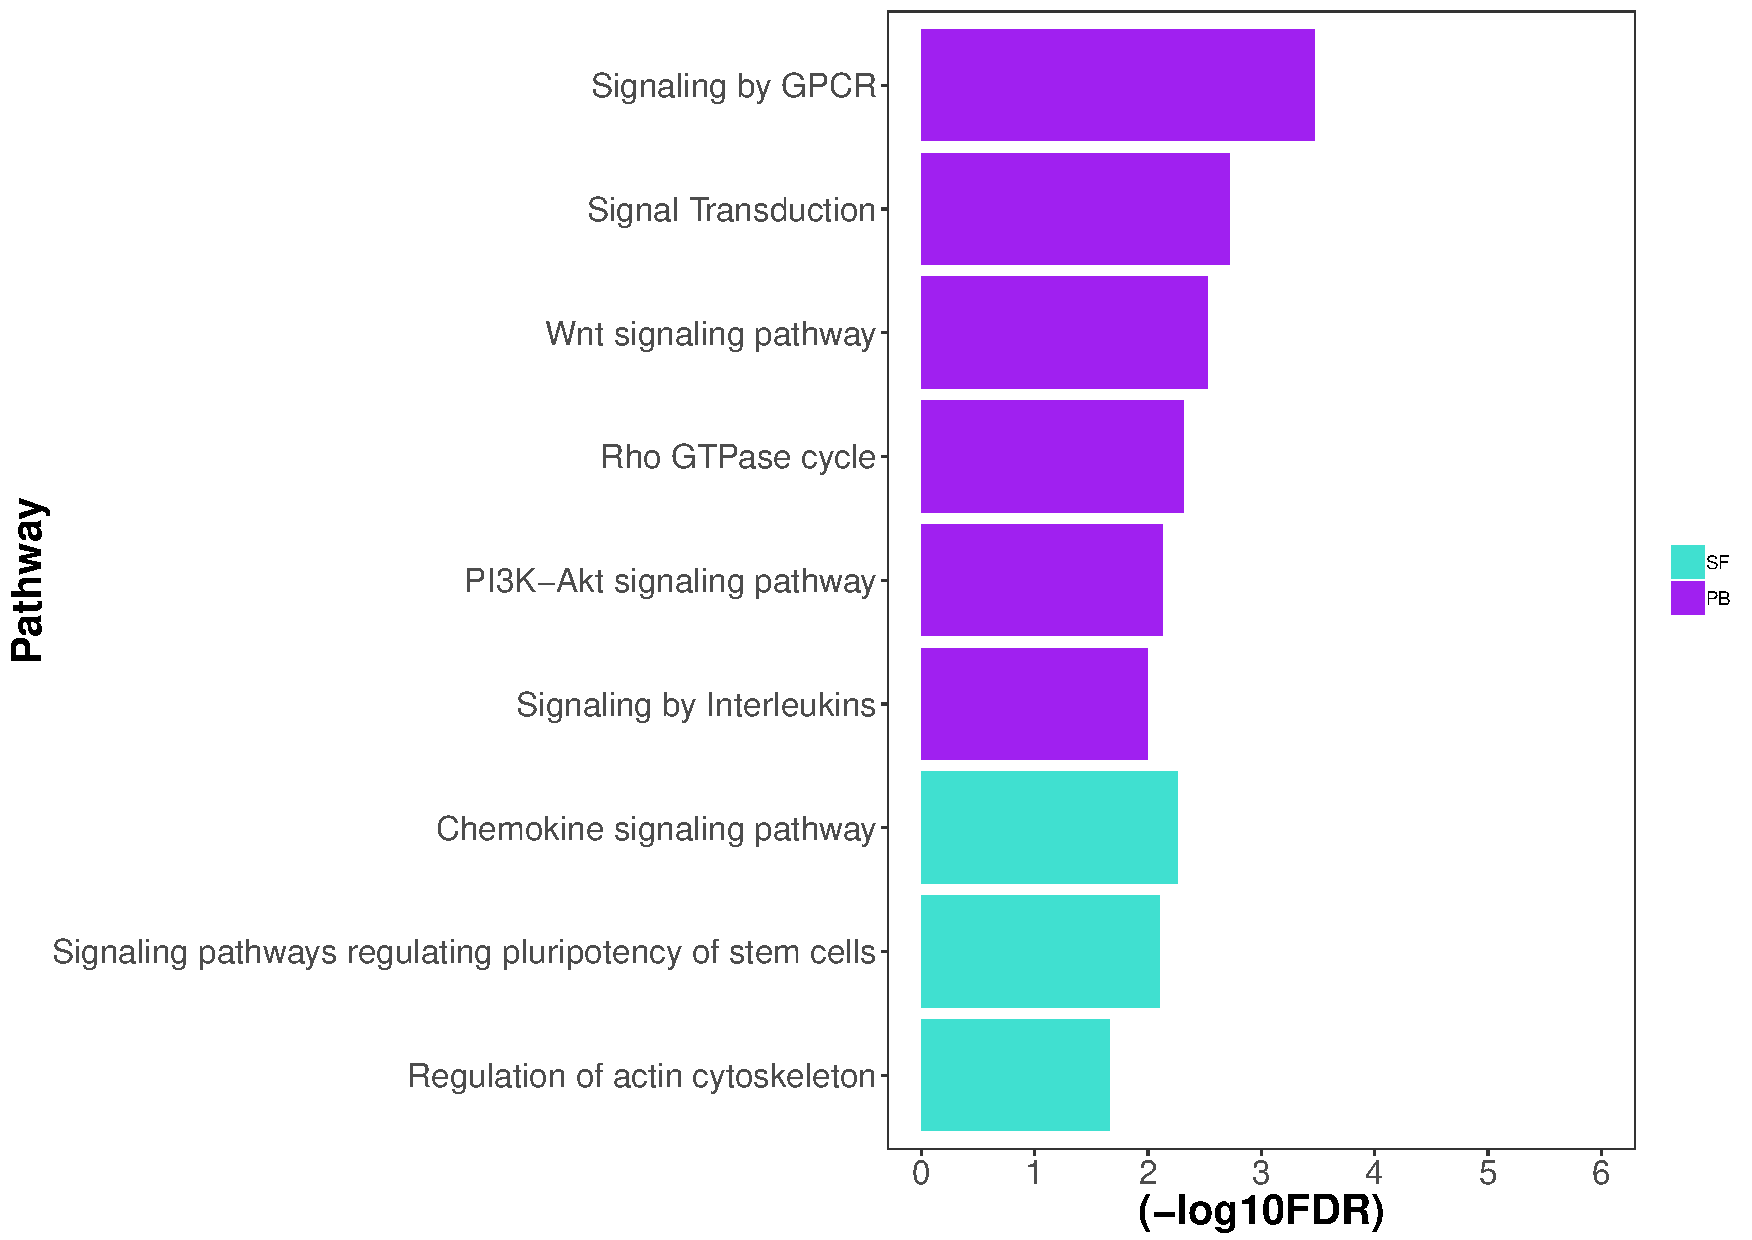
\includegraphics[width=\textwidth]{./Results3/pdfs/ATAC_PSA_CD8_pathways_barplot_all_DOCS_proximity}%
\caption{}
\end{subfigure}
\begin{subfigure}[b]{0.45\textwidth} 
%the [b] prevents offset in subcaptions
\centering
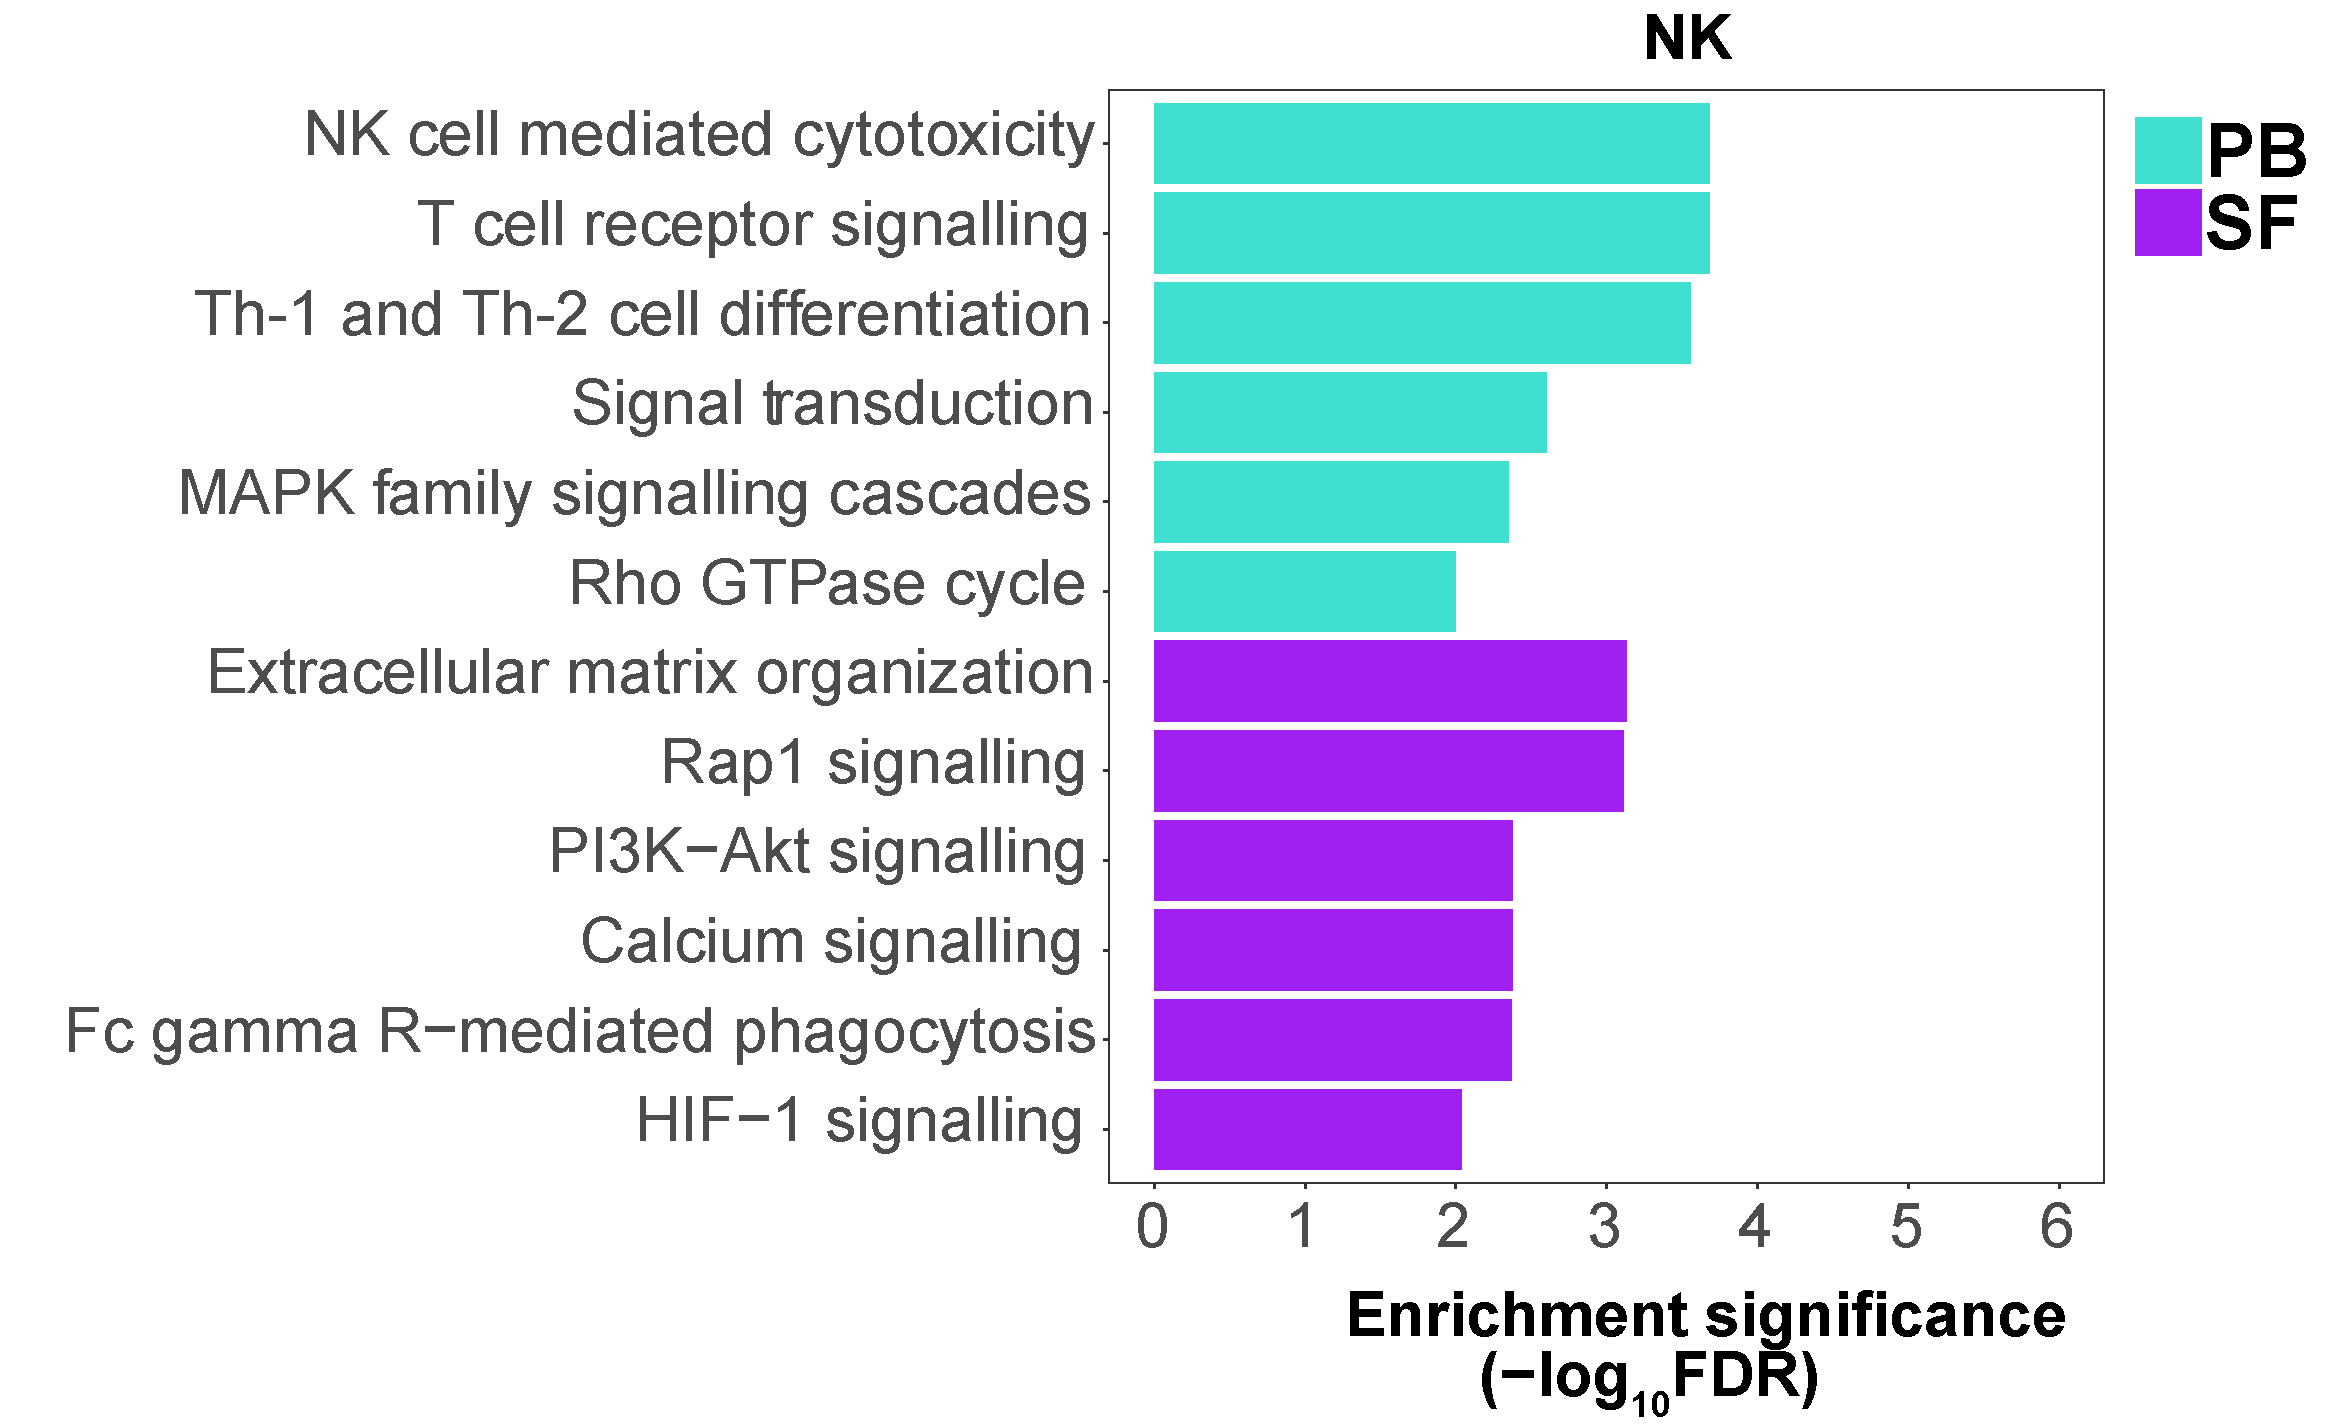
\includegraphics[width=\textwidth]{./Results3/pdfs/ATAC_PSA_NK_pathways_barplot_all_DOCS_proximity}%
\caption{}
\end{subfigure}
\caption[Distinct enriched pathways across SF and PB in CD14$^+$,CD4m$^+$,CD8m$^+$ and NK.]{\textbf{Distinct enriched pathways across SF and PB in CD14$^+$, CD4m$^+$, CD8m$^+$ and NK.} All pathways shown have an FDR $<$0.01.}
\label{figure:PSA_ATAC_pathway_analysis_all_DOC}
\end{figure}


%Decide if table or barplots
%\begin{landscape}
%\begin{center}
%\begin{longtable}[ht]{c c c }
%\caption[Distinct enriched pathways in CD14$^+$, mCD4$^+$, mCD8$^+$ and NK between SF and PB]{\textbf{Distinct enriched pathways in CD14$^+$, mCD4$^+$, mCD8$^+$ and NK between SF and PB.} All pathways shown have an FDR $<$0.01.}
%\\
%\label{table:PSA_ATAC_pathway_analysis_all_DOC} \\
%\toprule
%\textbf{Cell type} & \textbf{SF} & \textbf{PB} \\						
%\midrule
%\midrule
%CD14$^+$ & Hemostasis, Platelet activation, Signaling by VEGF & DAP12 interactions, Metabolism of lipids, \\ 
         %& GPCR ligand binding, IL-2 signaling pathway, & Metabolism of vitamins and co-factors, \\ 
         %& Integrin cell surface interactions,NF-kappa B signaling pathway & Negative regulation of the PI3K/AKT network. \\ 
         %& IL-2 family signaling, IL-3, 5 and GM-CSF signaling. & \\ 
%\midrule
%\textbf{mCD4$^+$} & T cell receptor signaling pathway, Phospholipase D signaling pathway ,& Signaling by Receptor Tyrosine Kinases,\\ 
									%& Chemokine signaling pathway, PI3K-Akt signaling pathway, & Focal adhesion.\\ 
									%& Signaling by interleukins. & \\
%\midrule
%\textbf{mCD8$^+$} & Chemokine signaling pathway, Signaling by GPCR  & Signal transduction, Wnt signaling pathway,\\ 
									%& Signaling pathways regulating pluripotency of stem cells & Rho GTPase cycle, PI3K-Akt signaling pathway, \\ 
									%& Regulation of actin cytoskeleton. & Signaling by interleukins. \\ 
%\midrule
%\textbf{NK$^+$} & Extracellular matrix organization, Rap1 signaling pathway, & Th1 and Th2 cell differentiation, Rho GTPase cycle,\\ 		
								%& Calcium signaling pathway, PI3K-Akt signaling pathway,     & T cell receptor signaling pathway, Signal Transduction,\\ 
								%& Fc gamma R-mediated phagocytosis, HIF-1 signaling pathway. & Natural killer cell mediated cytotoxicity,  \\
								%&                                                            & MAPK family signaling cascades.	\\ 								
%\bottomrule
%\medskip
%\end{longtable}
%\end{center}
%\end{landscape}


In addition to pathway level analysis, individual enrichment analysis for conserved TFBS within SF and PB open DORs in each cell type was conducted. To further enhance the reliability of the analysis, only DORs overlapping FANTOM5 eRNA expressed in that particular cell type were considered. 


\begin{figure}[htbp]
\centering
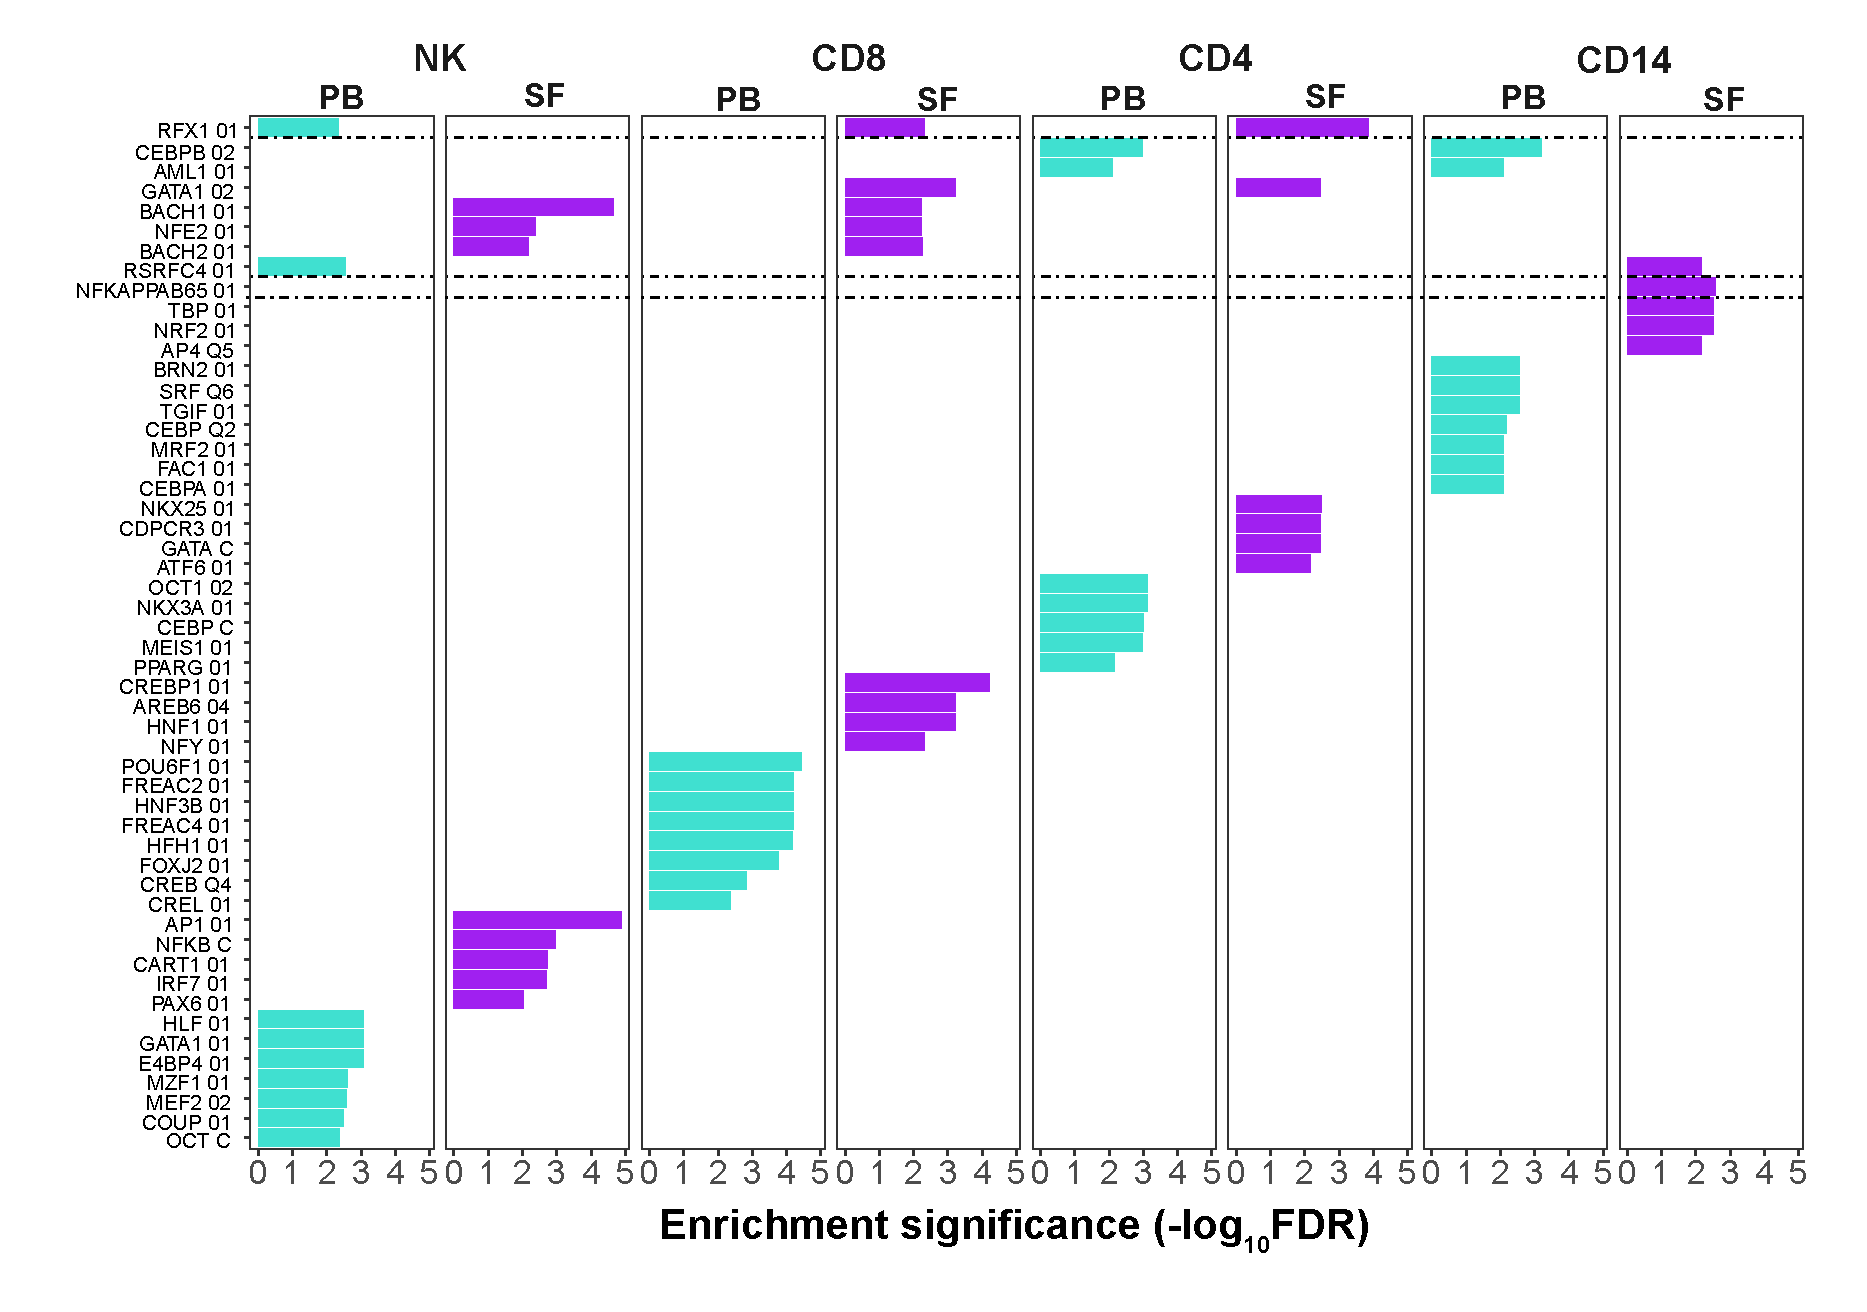
\includegraphics[width=0.8\textwidth]{./Results3/pdfs/ATAC_PSA_enrichment_conserved_TFBS_barplots_cell_type_specific_DOCS_all_cell_types_per_tissue}
\caption[Enrichment of eRNA cell type-specific PsA DORs for conserved TFBS.]{\textbf{Enrichment of eRNA cell type-specific PsA DORs for conserved TFBS.} xxxx }
\label{fig:PSA_TFBS}
\end{figure}


% Probably move to the appendix
-TFBS



\subsection{Differential gene expression analysis in paired circulating and synovial immune cells}

\subsubsection{Immune-relevant gene expression and correlation with chromatin accessibility}
%Introductory paragraph to link to ATAC-seq data
Mapping chromatin accessibility represents an informative tool to identify regulatory elements undergoing histone modifications, DNA methylation and TF binding, as previously explained. All those elements are involved in the regulation of gene expression, making the study of chromatin accessibility a good proxy for the inference of genes expression. Nevertheless, the characterisation of the chromatin landscape also presents some limitations, including the discordance between open chromatin and functionality of the regulatory element, shown by CAGE studies, as well as the identification of the target gene regulated by a particular element. 

In order to contextualise the ATAC-seq data, PCR gene expression analysis for 370 key genes in the inflammatory and autoimmune response was conducted in CD14$^+$ monocytes, mCD4$^+$ and mCD8$^+$ cells isolated from SF and PB of three PsA patients (Table \ref{tab:PSA_datasets_per_sample}). Those appeared as the most abundant cell types in PB and SF from patients and particularly for mCD8$^+$ cells have been shown to expand in PsA inflammed synovium, as previously mentioned. The PCR array represented a cost-effective approach to study gene expression between PB and SF focusing in a relevant subset of genes of notably importance, given the pathophysiological characteristics of PsA. In each cell types, fold-change (FC) in expression was calculated pair-wise for SF in respect to PB within each sample for each of the tested genes. Likely due to the small sample size, most of the modulated genes between SF and PB lacked of significance after multiple testing correction (FDR$<$0.05). Therefore, to explore biological relevance of this data, pval$<$0.05 was used as the filtering threshold. 

% Since I am not used corrected pval Hai mentioned that I can not talk about differentially expressed
When exploring for each individual and each cell type, %When considering all the significantly modulated genes (pval$<$0.05) in at least one cell type, 
differences in magnitude and reproducibility in FCs were observed across samples and cell types (Figure \ref{figure:PSA_PCR_array_5pcnt_heatmap}). Some of the modulated genes showed upregulation (log$_2$FC$>$0) in SF compared to PB across the three cell types, for example \textit{IFN1}, \textit{SPP1} or \textit{CCL2}, amongst others (Figure \ref{figure:PSA_PCR_array_5pcnt_heatmap} orange). On the other hand, a number of genes presented reduced expression in SF (log$_2$FC$<$0) in at least one of the three cell types, including \tetxtit{FOS}, \textit{IL16}, \textit{PPBP} and \textit{TPST1} (Figure \ref{figure:PSA_PCR_array_5pcnt_heatmap} purple). Also, a number of only seemed consistently modulated in CD14$^+$ monocytes but not in T cells (Figure \ref{figure:PSA_PCR_array_5pcnt_heatmap} dark blue). For example, \textit{CCR7} and \textit{IL7R} were upregulated in SF CD14$^+$ monocytes compared to PB; however the FCs between SF and PB were largely variable across the three patients in mCD4$^+$ and mCD8$^+$. Moreover, differences in the magnitude of FCs across the three cell types were observed for some of the genes modulated in the same direction across the three cell types, for instance \textit{VEGFB} and \textit{CXCR6} (Figure \ref{figure:PSA_PCR_array_5pcnt_heatmap} black and green).

\begin{landscape}
\begin{figure}[H]
\centering
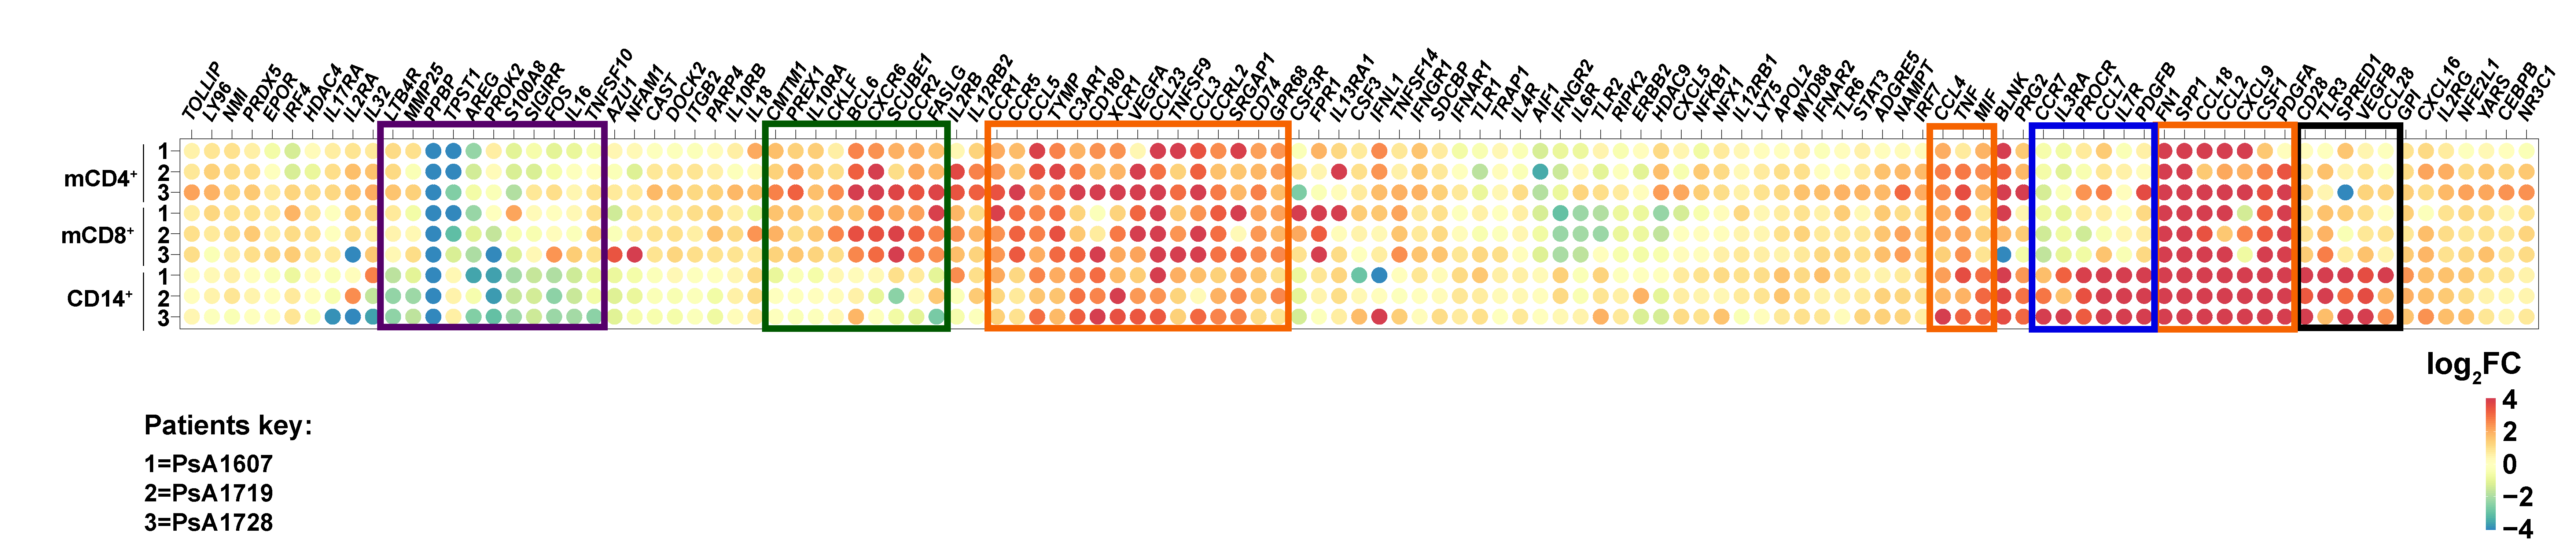
\includegraphics[width=1.5\textwidth]{./Results3/pdfs/PCR_array_PSA_SF_vs_PB_filtered_5_percent_genes_heatmap}
\caption[Representation of the fold-change in gene expression between SF and PB for the significant genes (pval$<$0.05) in at least one of the cell types.]{\textbf{Representation of the fold-change in gene expression between SF and PB for the significant genes (pval$<$0.05) in at least one of the cell types.} xxxx }
\label{fig:PSA_PCR_array_5pcnt_heatmap}
\end{figure}
\end{landscape}


Further filtering based on statistical significance (pval$<$0.05) and FCs (0.6$<$FC$<$1.5), revealed that CD14$^+$ monocytes and mCD8$^+$ presented greater number of significantly modulated (70 and 73 genes, respectively) compared to mCD4$^+$ cells (46 genes) (Figure \ref{figure:PSA_PCR_array_vulcano_plots} a, b and c). For the three analysed cell types, the majority of modulated immune genes presented upregulation in the SF (Figure \ref{figure:PSA_PCR_array_vulcano_plots} a, b and c). For example, 56 out of the 70 significantly modulated genes in CD14$^+$ monocytes showed a log$_2$ mean FC$>$0.586 versus the 14 genes with log$_2$mean FC$<$-0.586 (Figure \ref{figure:PSA_PCR_array_vulcano_plots} a).



% May need a bit more of biology there
\begin{figure}[htbp]
\centering
\begin{subfigure}{0.5\textwidth}
\centering
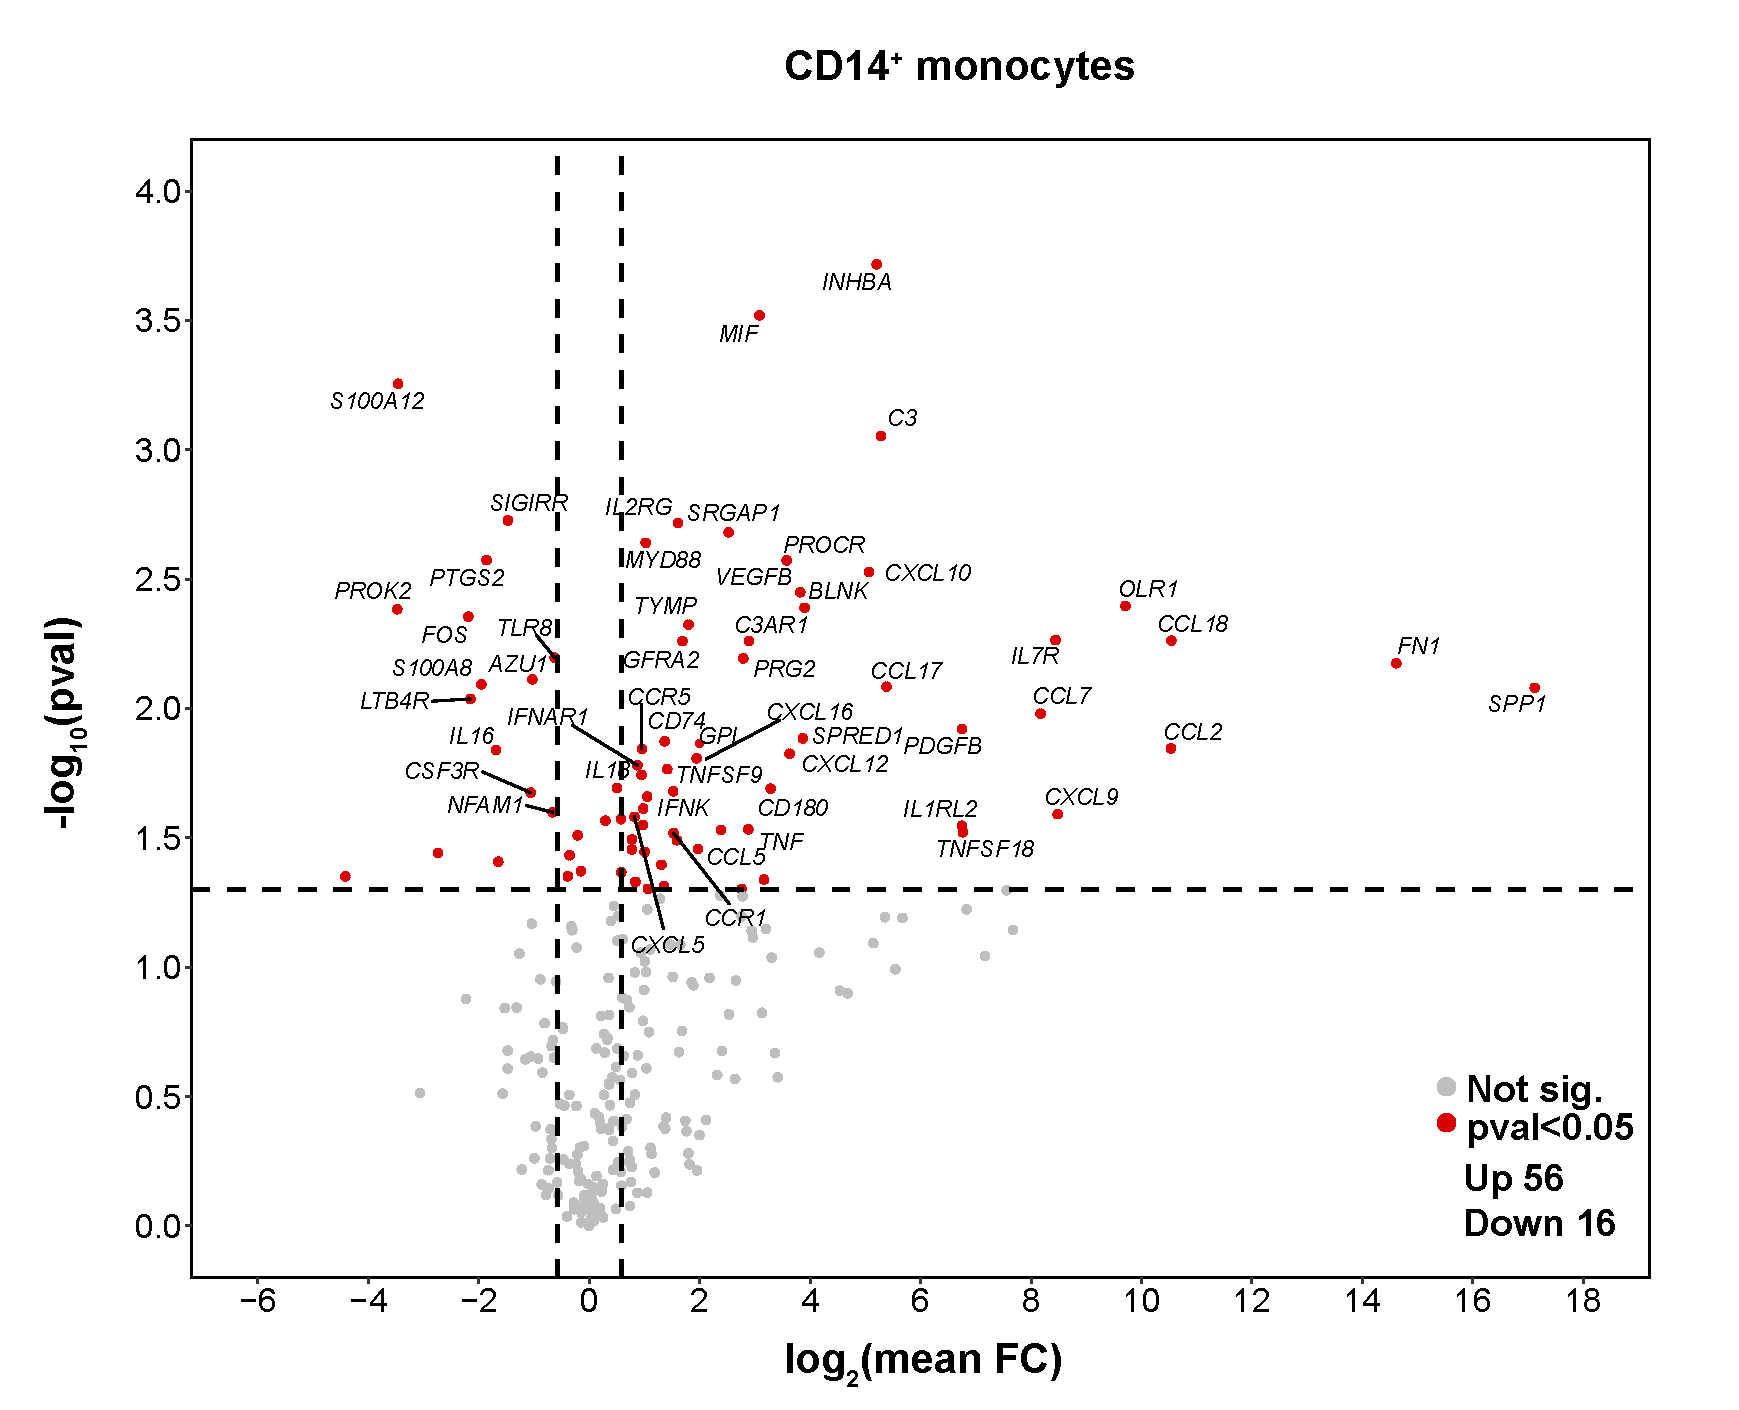
\includegraphics[width=\textwidth]{./Results3/pdfs/PSA_CD14_vulcano_plot_PCR_array_mean_FC}
\caption{\textbf{}}
% The percentage sign indicated that the other subfig goes side by side
\end{subfigure} \\
\begin{subfigure}{0.5\textwidth}
\centering
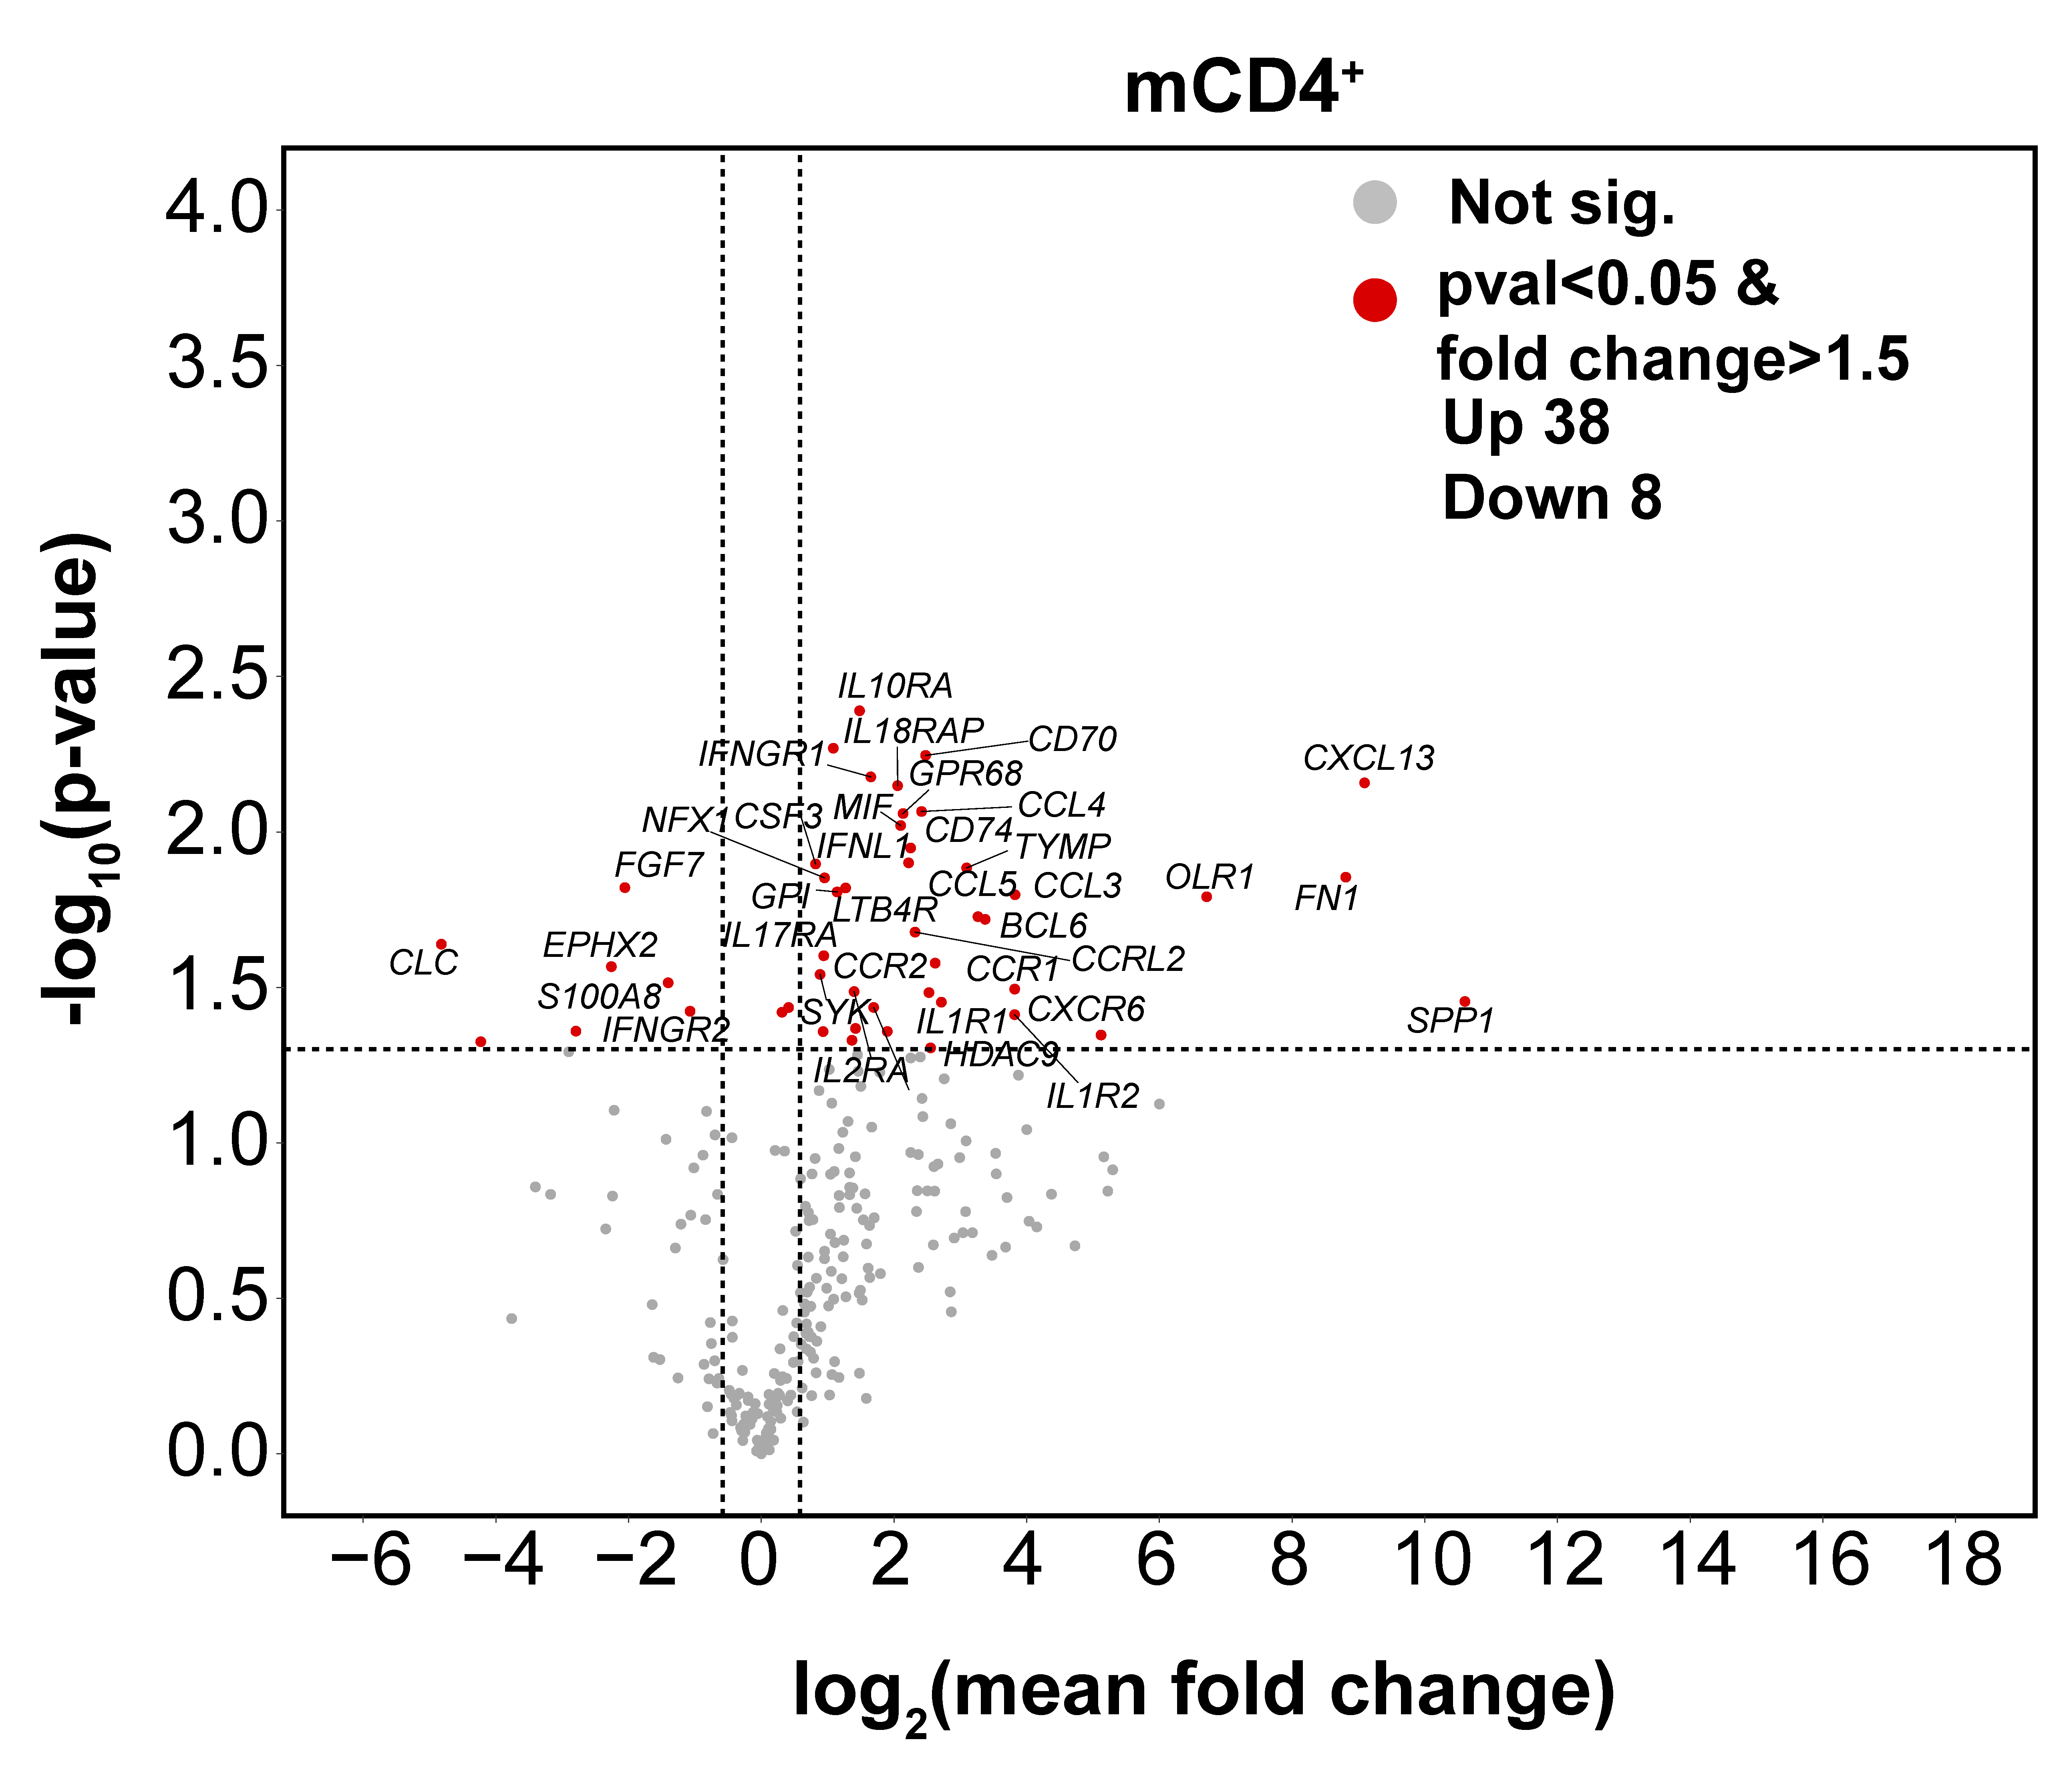
\includegraphics[width=\textwidth]{./Results3/pdfs/PSA_CD4_vulcano_plot_PCR_array_mean_FC}
\caption{\textbf{}}
\end{subfigure} %
\begin{subfigure}{0.5\textwidth}
\centering
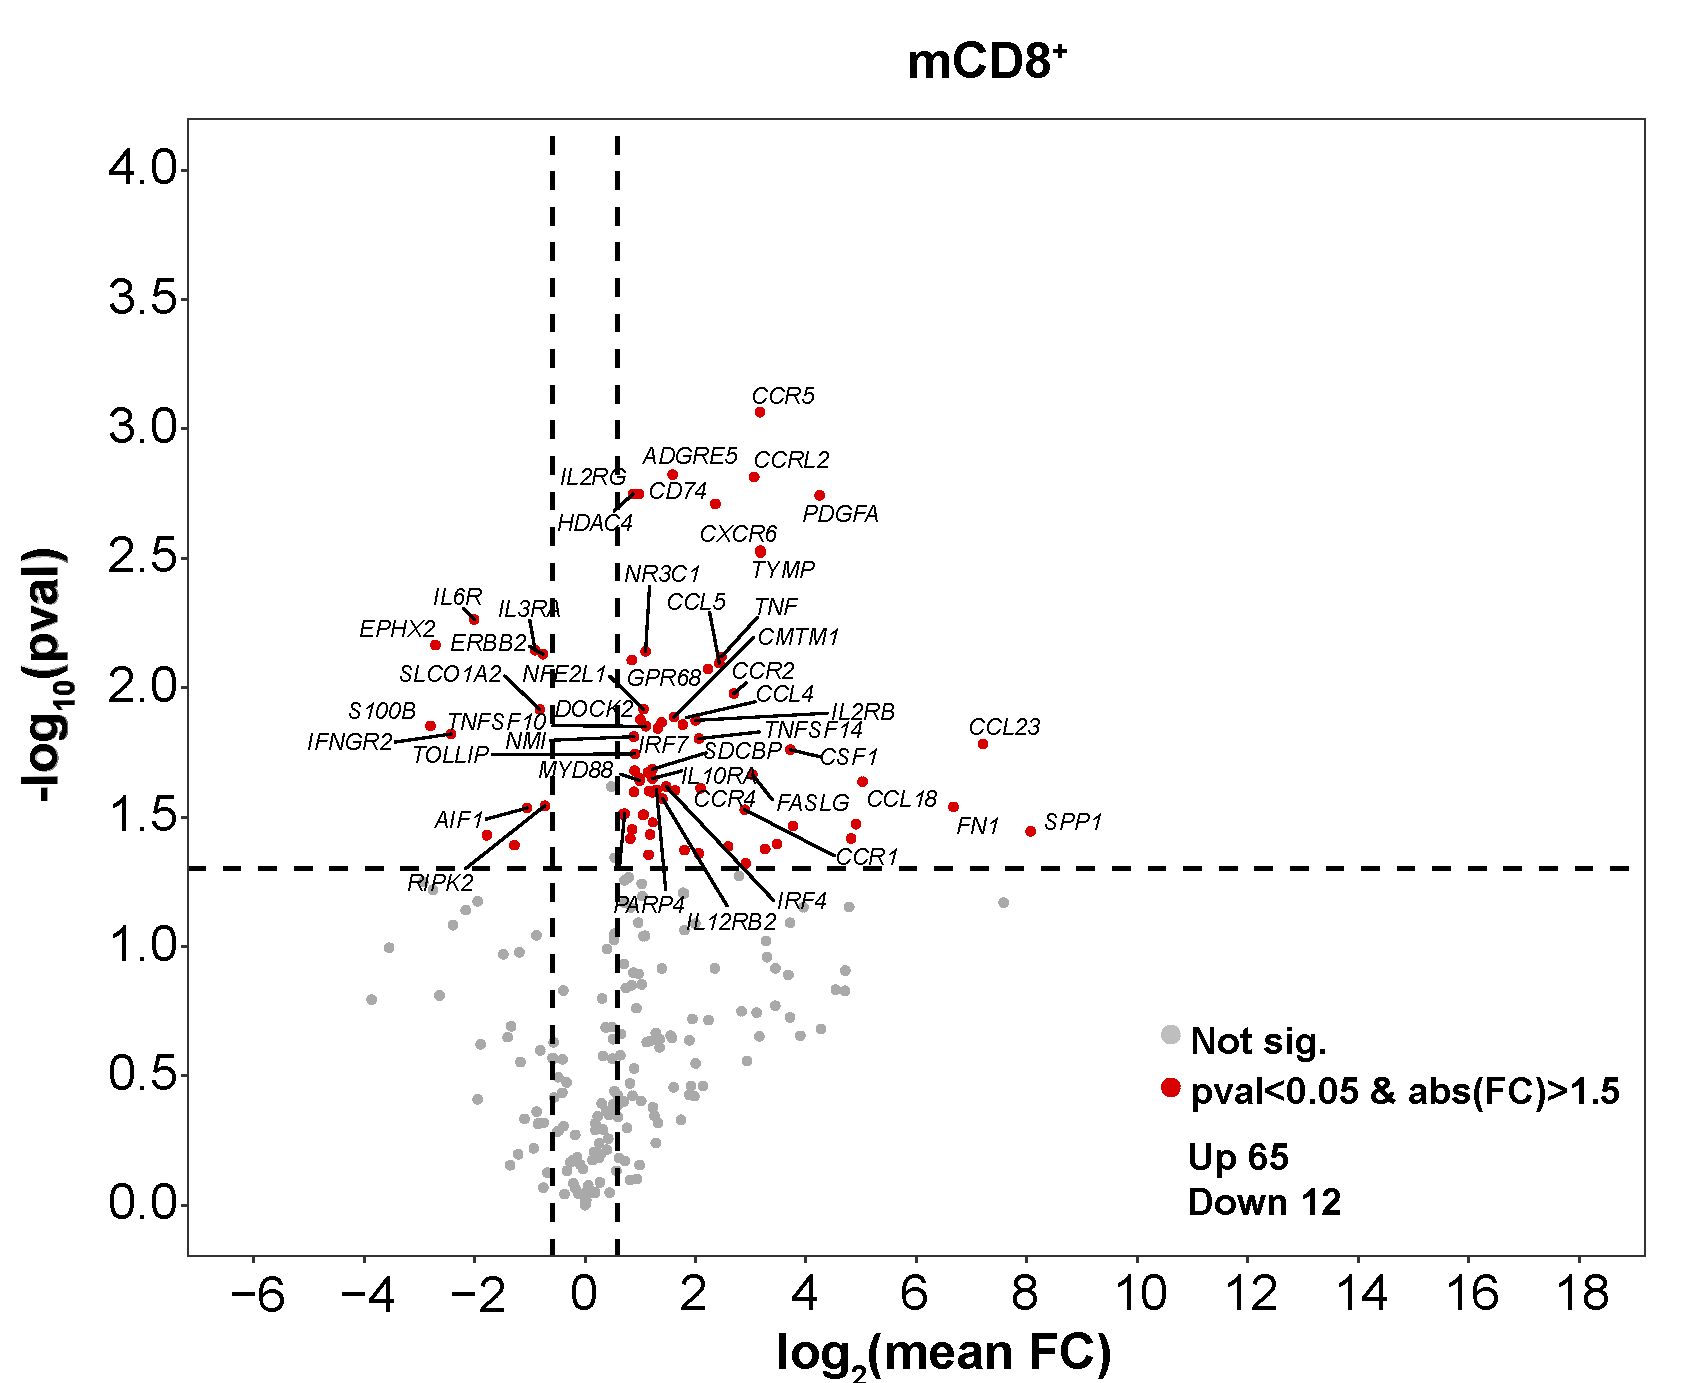
\includegraphics[width=\textwidth]{./Results3/pdfs/PSA_CD8_vulcano_plot_PCR_array_mean_FC}
\caption{\textbf{}}
\end{subfigure}
\caption[Expression changes in immune-relevant genes between SF and PB in CD14$^+$ monocytes, mCD4$^+$ and mCD4$^+$ cells.]{\textbf{Expression changes in immune-relevant genes between SF and PB in CD14$^+$ monocytes, mCD4$^+$ and mCD4$^+$ cells.}}
\label{fig:PSA_PCR_array_vulcano_plots}
\end{figure} 



% ATAC overall overlap
Amongst the significantly modulated genes (based on pval and FC cut-offs) between SF and PB, overlap with DORs were observed for the three cell types (Table \ref{tab:PSA_gene_expression_ATAC_overlap}). In CD14$^+$ monocytes, 13 out of the 56 significantly upregulated genes in SF overlapped with DORs more accessible in this tissue. 


\begin{table}[htbp]
%\setlength{\tabcolsep}{20pt} only to stretch the columns if you want
%\renewcommand{\arraystretch}{1.5}
\centering
\begin{tabular}{@{} c c c}
\toprule
\textbf{Cell type} & \textbf{Genes upregulated and}        &  \textbf{Genes downregulated and} \\
                   & \textbf{overlapping open chromatin}   &  \textbf{ overlapping closed chromatin} \\
									 &	\textbf{ in SF}				               &  \textbf{in SF} \\
\midrule
\midrule
CD14$^+$ & 13 (\textit{BLNK}, \textit{CCL2$^\ast$}, \textit{CCR1$^\ast$}, \textit{CD180}, & 2 (\textit{FOS}, \textit{PROK2$^\ast$}) \\
				 & \textit{CXCL10}, \textit{FN1}, \textit{IL18}, \textit{IL31RA$^\ast$},    & \\
				 & \textit{IL7R$^\ast$}, \textit{NFKB1$^\ast$}, \textit{PRG2}, \textit{SRGAP1}, & \\
				 & \textit{STAT3}) & \\
				
\midrule
CD4$^+$ & 3 (\textit{CXCL13}, \textit{CXCR6$^\ast$}), \textit{IL2RA}& 0 \\

\midrule
CD8$^+$ & 6 (\textit{CCL3}, \textit{CCR2}, \textit{CCR5} ,\textit{IRF4} & 1 (\textit{EPHX2}) \\
        & \textit{TNFSF10}, \textit{YARS}) & \\

\bottomrule
\end{tabular}
\medskip %gap
\caption[Immune genes with significant modulated expression in SF proximal to a DOR in ATAC-seq.]{\textbf{Immune genes with significant modulated expression in SF proximal to a DOR in ATAC-seq.} An overlap is defined by significant change in expression (pval$<$0.05) of a particular gene where there is also a proximal DOR showing changes in chromatin accessibility in the same direction. ($^\ast$) indicates that the proximal DOR overlapping an eRNA identified by FANTOM5 project in that particular cell type (see subsection Characterisation of the differential accessible chromatin regions).}
\label{tab:PSA_gene_expression_ATAC_overlap}
\end{table}

For example, the greater chromatin accessibility at the \textit{IL7R} 5' and 3' UTR, previously shown (Figure \ref{figure:PsA_FAST_ATAC_gene_boy_DOCS_CD14_NK} b) correlated with greater mRNA expression in SF CD14$^+$ monocytes. Another relevant example is the \textit{FN1}, involved in cell adhesion, migration and osteoblast biology. Upregulated expression in synovial biopsies compared to PB has already been reported \parencite{Dolcino2015}. In this cohort, \textit{FN1} expression was upregulated in SF for all three cell types, with the greater FC found in CD14$^+$ monocytes (Figure \ref{figure:PSA_PCR_array_vulcano_plots} a), concomitantly with more accessible chromatin at the promoter and 3' UTR of the gene (Figure \ref{figure:PSA_CD14_ATAC_FN1}). Lesser overlap between gene expression and chromatin accessibility was observed in mCD4$^+$ and mCD8$^+$ (6 and 3 targets, respectively) between genes with greater expression and accessible chromatin in SF compared to PB. Only significantly downregulated genes in CD14$^+$ monocytes and mCD8$^+$ isolated from SF presented overlap with proximal less accessible chromatin regions (2 and 1, respectively) in the same tissue. 
%decide which example to use: I have included IL7R in monocytes and maybe could use FN1 to complete
	%Example expression in CD14 FOS,FN1,CCL2,CXCL10
	
\begin{figure}[htbp]
\centering
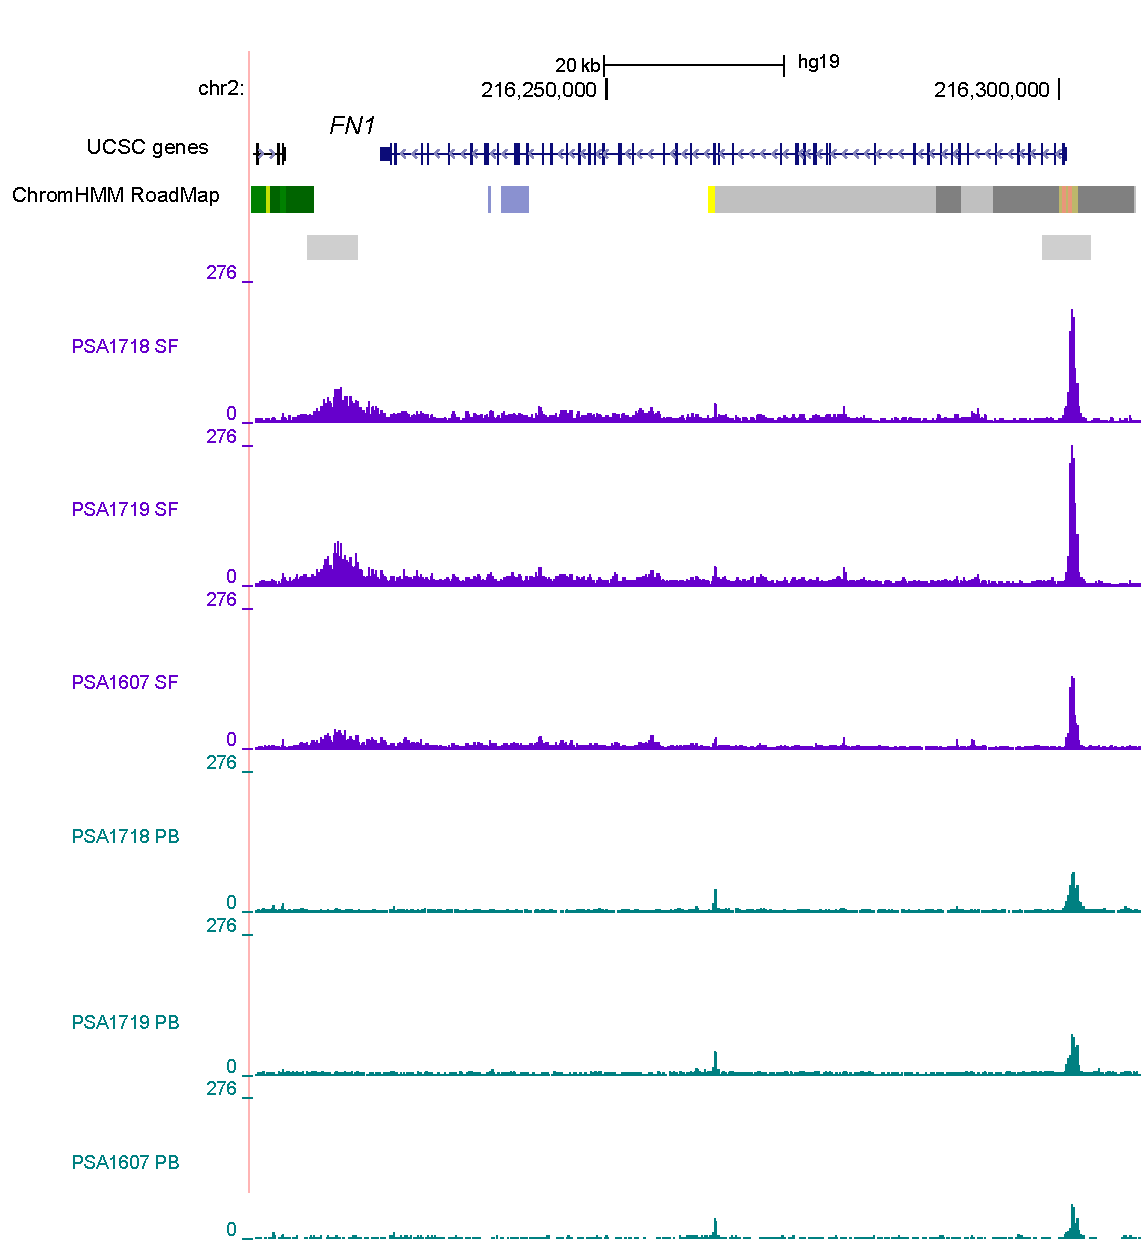
\includegraphics[width=0.6\textwidth]{./Results3/pdfs/PSA_CD14_ATAC_FN1_paired_gene_expression}
\caption[Chromatin accessibility at the \textit{FN1} gene in CD14$^+$ monocytes isolated from SF and PB.]{\textbf{Chromatin accessibility at the \textit{FN1} gene in CD14$^+$ monocytes isolated from SF and PB.} xxxx }
\label{fig:PSA_CD14_ATAC_FN1}
\end{figure}

\subsubsection{Pathway enrichment and network analysis highlights the role of synovial CD14$^+$ monocytes in cytokine and chemokine production}
\subsubsection{Modulated gene expression in CD14$^+$ monocytes shows enrichment for cytokine and chemokine production}
%Describe pathway analysis results and curate the pathway of interest
To identify relevant pathways amongst the modulated genes between SF and PB, enrichment analysis was performed for each of the three cell types. Upregulated and downregulated genes showing 0.6$<$ mean FC $>$1.5 and pval$<$0.05 were combined for the analysis. Interestingly, the modulated genes between SF and PB in CD14$^+$ monocytes were enriched for chemokine, NOD-like signalling and TLR signalling pathways (Table \ref{table:PSA_PCR_array_pathway_analysis}). All three pathways are involved in the activation of cytokines and chemokines gene expression, leading to T cell recruitment and inflammatory response. 

The TLR signalling pathways enrichment involved \textit{FN1} (previously mentioned) and \textit{SPP1}, two of the top three most differentially expressed genes reported by Dolcino and colleagues in a study comparing synovial biopsies between healthy and PsA individuals \parencite{Dolcino2015} (Table \ref{table:PSA_PCR_array_pathway_analysis}). Together with \textit{FN1}, \textit{SPP1} was also highly upregulated (mean log$_2$FC$\geq$4) in the three cell types (Figure \ref{figure:PSA_PCR_array_5pcnt_heatmap} orange), showing the greatest FC in monocytes (Figure \ref{figure:PSA_PCR_array_vulcano_plots} a). Moreover, some of the genes driving enrichment, such as \textit{CCL5} and \textit{NFKB}, were also shared across the three pathways of interest. Others genes, including \textit{TNF}, \tetxit{IRF7} and \textit{MyD88}, highlighted the cross-link between the NOD-like and the TLR signalling pathways. The enrichment of SF open chromatin regions in CD14$^+$ monocytes for the NF$\kapa$B pathway is closely related to the enrichment for TLR and NOD-like signalling pathways at the transcriptomic level (Figure \ref{figure:PSA_ATAC_pathway_analysis_all_DOC} a). Both, TLR and NOD-like pathways lead to the activation of the NF$\kapa$B TF, which induces transcriptional activation of pro-inflammatory cytokines, also supported by the enrichment of SF more accessible DORs for IL-2, IL-3, IL-5 and GM-CSF pathways (Figure \ref{figure:PSA_ATAC_pathway_analysis_all_DOC} a). Moreover, the pivotal role of NF$\kappa$B in the immune transcriptional profile of SF CD14$^+$ monocytes  is additionally sustained at the chromatin accessibility level by the enrichment of SF accessible chromatin sites for this TF (Figure \ref{figure:PSA_TFBS}).  

The enrichment for the chemokine pathway in CD14$^+$ monocytes (Table \ref{table:PSA_PCR_array_pathway_analysis}) included modulated genes highly upregulated (mean log$_2$FC$\geq$4) in SF compared to PB (e.g \textit{CCL18} and \textit{CCL2}) for all three cell types (Figure \ref{figure:PSA_PCR_array_5pcnt_heatmap} orange) as well as genes only consistently modulated between SF and PB in CD14$^+$ monocytes (e.g \textit{CCL28}, Figure \ref{figure:fig:PSA_PCR_array_5pcnt_heatmap} black). This pathway involves production of chemotractant molecules involved in the recruitment of leukocytes to the site of inflammation and the production of reactive oxygen species (ROS) through Ca$^2$$^+$ mobilisation, a pathway presenting enrichment for more accessible chromatin regions in SF CD14$^+$ monocytes (Figure \ref{figure:PSA_ATAC_pathway_analysis_all_DOC} a).

At the transcriptional level, significantly modulated genes between SF and PB in mCD4$^+$ T cells were enriched for the IL-10 signalling pathway (Table \ref{table:PSA_PCR_array_pathway_analysis}), in lines with the enrichment for IL signalling of open chromatin in SF cells (Figure \ref{figure:PSA_ATAC_pathway_analysis_all_DOC} b). 


\begin{landscape}
\begin{center}
\begin{longtable}[ht]{c c c }
\caption[Pathway enrichment analysis for the modulated genes between SF and PB in CD14$^+$ and mCD4$^+$.]{\textbf{Pathway enrichment analysis for the modulated genes between SF and PB in CD14$^+$ and mCD4$^+$.} The analysis was performed using only those genes showing 0.5$<$mean fold-changes$>$1.5 across the three patients and pval$<$0.05. Enriched pathways based on FDR $<$0.05.}
\\
\label{table:PSA_PCR_array_pathway_analysis} \\
\toprule
\textbf{Cell type} & \textbf{Pathway} & \textbf{Genes} \\						
\midrule
\midrule
\textbf{CD14$^+$} & Chemokine signalling & \textit{CCL17}, \textit{CCL18}, \textit{CCL2}, \textit{CCL28}, \textit{CCL5}, \textit{CCL7}, \textit{CCR1}, \textit{CCR5},\textit{CXCL10} \\  
									&                             & \textit{CXCL12}, \textit{CXCL16}, \textit{CXCL5}, \textit{CXCL9}, \textit{NFKB1}, \textit{PPBP}, \textit{PF4V1}, \textit{STAT3}, \textit{XCR1}\\
									
									& NOD-like receptor signalling & \textit{CCL2}, \textit{CCL5}, \textit{IFNAR1}, \textit{IL18}, \textit{IRF7}, \textit{MEFV}, \textit{MYD88}, \textit{NFKB1}, \\
									&                                         & \textit{NAMPT}, \textit{TNF} \\

									& TLR signalling   & \textit{CCL5}, \textit{CXCL10}, \textit{CXCL9}, \textit{IFNAR1}, \textit{IRF7}, \textit{MYD88}, \textit{NFKB1}, \textit{SPP1},\textit{FOS},\\ 
									&                                         & \textit{TLR1}, \textit{TLR2}, \textit{TLR8}, \textit{TNF}\\

\midrule
\textbf{mCD4$^+$} & IL-10 signaling & \textit{CCL3}, \textit{CCL4}, \textit{CCL5}, \textit{CCR1}, \textit{CCR2}, \textit{CSF1}, \textit{CSF3}, \textit{IL10RA}, \\
									&									& \textit{IL1R1}, \textit{IL1R2}\\
\bottomrule
\medskip
\end{longtable}
\end{center}
\end{landscape}

In addition to pathway enrichment, network analysis was performed to understand the interaction and relationship between the analysed genes. A gene subnetwork was identified from the STRING functional interaction database using as input the filtered expression PCR array information and ranking the genes based on the best pval across the three cell types. The identified subnetwork predominantly included  significant modulated genes between SF and PB. Amongst the most interesting node, the single Ig and Toll-interleukine domain containing gene (\textit{SIGRR}) which is a negative regulator of the TLR signalling pathway (Figure \ref{figure:PSA_PCR_network_analysis}). \textit{SIGIRR} is significantly downregulated in SF CD14$^+$ monocytes only and it is consistent with the significant upregulation (pval<0.05) of \textit{TLR1}, \textit{TLR2}, \textit{MyD88} and the enrichment for the TLR pathway in this cell type (Figure \ref{figure:PSA_PCR_array_5pcnt_heatmap} and \ref{table:PSA_PCR_array_pathway_analysis}). Moreover, the significant upregulation of \textit{NFKB} and \textit{TNF} in the SF CD14$^+$ monocytes could be a downstream result of the functional connection with TLR pathway members such as \textit{MyD88} and as a downstream result of the TLR signalling pathway. Conversely, in mCD4$^+$ and mCD8$^+$ the modulation of these members did not appear to be significant between SF and PB. However, in mCD8$^+$ \textit{TNF} is also significantly upregulated in the synovium. 

Another interesting part of the network is the connection of the TLR pathway and the chemokine production through \textit{NF$\kappa$B}, \textit{TNF} and \textit{CCL2} (Figure \ref{figure:PSA_PCR_network_analysis}). \textit{CCL2} is connected to \textit{CXCL10} and subsequently with \textit{CCL18} and \textit{CCR5}, all chemokines regulating migration and infiltration of monocytes and memory T cells. This network analysis also highlighted relationship between \textit{IL7R} and \textit{IL2RG} coding for the two chains of the IL-7 receptor (IL-7R). Interestingly, these two nodes are only significantly upregulated in SF CD14$^+$ monocytes, supporting a novel the cell and context specific role of IL-7R and polymorphism in this gene in this cell type under inflammatory conditions % Hussein paper

% I could also talk about the FOS, PROK2 and PTGS2

\begin{figure}[htbp]
\centering
\includegraphics[width=\textwidth]{./Results3/pdfs/PSA_PCR_array_network_analysis}
\caption[Protein network analysis based on the immune PCR array expression data.]{\textbf{Protein network analysis based on the immune PCR array expression data.} xxxx }
\label{fig:PSA_PCR_network_analysis}
\end{figure}

Overall, the integration of the chromatin accessibility and immune transcriptional data reinforced a relevant role of synovial CD14$^+$ monocytes in the production of cytokines and chemokines, leading to activation of the innate immune response and the recruitment of T cells to this site of inflammation. 




\subsubsection{Tissue and disease specificity in gene expression modulation and relevant biological pathways}

In order to better understand the disease and tissue specificity of the prior transcriptomic results, gene expression was analysed in CD14$^+$ monocytes, mCD4$^+$ and mCD8$^+$ isolated from PB in three healthy controls (HC) using the same PCR array. In each of the cell types, the FC in  was calculated for the PsA PB expression in respect to the healthy controls. Similarly to the previous analysis, pvals were calculated for the FC in each of the particular genes. When comparing to the modulated gene expression between SF and PB in PsA, three group of genes could be identified (Figure \ref{figure:PSA_PCR_array_HC_FC_correlation}). The genes only significantly modulated (based on pval and FC threshold criteria) in PB between HC and PsA were designated as systemic genes (Figure \ref{figure:PSA_PCR_array_HC_FC_correlation} green). Those genes were not significantly modulated in this data when comparing SF versus PB within PsA patients and could then be considered as the circulating disease "footprint". In this respect, CD14$^+$ monocytes was the cell type with lower number of systemic modulated genes (14), compared to mCD8$^+$ (23) and mCD4$^+$ (42) (Figure \ref{figure:PSA_PCR_array_HC_FC_correlation}a, b and c). 

Another group of genes were designated as tissue specific, since they were significantly modulated between SF and PB in PsA patients but did not show significant changes between HC and PsA at the circulating level (Figure \ref{figure:PSA_PCR_array_HC_FC_correlation} red). Interestingly, in CD14$^+$ monocytes the tissue specific modulated genes considerably outnumber the systemic ones (62 versus 14), showing a more pronounced change in the expression profile of immune genes across patients tissues than between healthy and diseased PB (Figure \ref{figure:PSA_PCR_array_HC_FC_correlation} a in red). For example, the aforementioned \textit{NFKB} and \textit{MyD88}, \textit{TLR2} genes were only upregulated in PsA SF CD14$^+$ monocytes and their expression was not significantly modulated between HC and PsA circulating CD14$^+$ monocytes.  Similarly to CD14$^+$ monocytes, mCD8$^+$ cells also presented greater disease tissue-specific modulation than genes modulated compared to HC in PB (Figure \ref{figure:PSA_PCR_array_HC_FC_correlation} c in red).  
%Some more biology?
% talk about limitations in acknowledging these genes as dissease-tissue specific due to the fact that we don't know if they also change between PB and Sf in HV

The third category of genes were those significantly modulated for each cell type between HC and PsA patients in PB as well as between SF and PB from PsA individuals. These were defined as putative disease-specific genes and numbers were similar across CD14$^+$ monocytes, mCD4$^+$ and mCD8$^+$ (10, 9 and 8, respectively) (Figure \ref{figure:PSA_PCR_array_HC_FC_correlation} blue in a, b and c). In CD14$^+$ monocytes two of those genes, \textit{GPI} and \textit{PRG2}, were upregulated in both comparisons with further exacerbation in SF when comparing the log$_2$FCs (Figure \ref{figure:PSA_PCR_array_HC_FC_correlation} a). Evidence of the glucose-6-phosphate isomerase \textit{GPI} upregulation has been found in RA synovial fibroblast and linked to increased levels of TNF-$\alpha$ and IL-1$\beta$ in the synovium \parencite{Zhong2015}. % GPI fibroblasts https://www.ncbi.nlm.nih.gov/pmc/articles/PMC4422595/
Another example of exacerbated upregulation in SF was the expression of \textit{GPR68} in mCD4$^+$. This gene was upregulated in PsA PB mCD4$^+$ when compared to the HC counterparts and further upregulated in SF when compared to PB in PsA individuals (Figure \ref{figure:PSA_PCR_array_HC_FC_correlation} b). \textit{GPR68} is a G protein-coupled receptor, expressed in T cells , amongst others, which gets activated through pH acidification, particularly relevant in synovial tissues, increasing Ca$^2$$^+$ levels and leading to activation of immune pathways. \textit{GPR68} was also upregulated in SF compared to PB in mCD8$^+$ cells, reinforcing the relevance of this gene in the synovial pathophysiological aspect of PsA. An opposite example is the epidermal growth factor-like amphiregulin (\textit{AREG}) gene which is significantly upregulated in PsA PB mCD8$^+$ cells compared to the HV but is downregulated in SF compared to PB in mCD8$^+$ from PsA individuals (Figure \ref{figure:PSA_PCR_array_HC_FC_correlation} c). Lack of \textit{AREG} in mouse models have been shown an impaired immunosupressive response by Treg cells \parencite{Zaiss2013}. 
% GPR68 https://ard.bmj.com/content/73/Suppl_2/511.2
%talk about limitations of those genes to be identified as disease specific. This would need an additional comparison between HV SF and PsA SF to make sure that those genes are not modulated in SF of HV and therefore are a lanmark of disease in both tissues

Despite the interesting findings, the identification of disease-specific and disease tissue-specific genes is clearly limited by the lack of HC SF in the experimental design, partly due to invassive sampling procedure, and further commented in the Discussion.

When performing pathway enrichment analysis using the significantly modulated genes between healthy and PsA patients PB, none specific pathway enrichment beyond Reactome immune system were identified only for CD14$^+$ monocytes and mCD4$^+$. This result reinforced the tissue-specificity of the pathways enriched for the modulated genes between SF and PB in CD14$^+$ monocytes PsA patients and clearly suggest a more pronounced inflammatory phenotype of the pathological CD14$^+$ monocytes in SF compared to PB.

\begin{figure}[htbp]
\centering
\begin{subfigure}{0.5\textwidth}
\centering
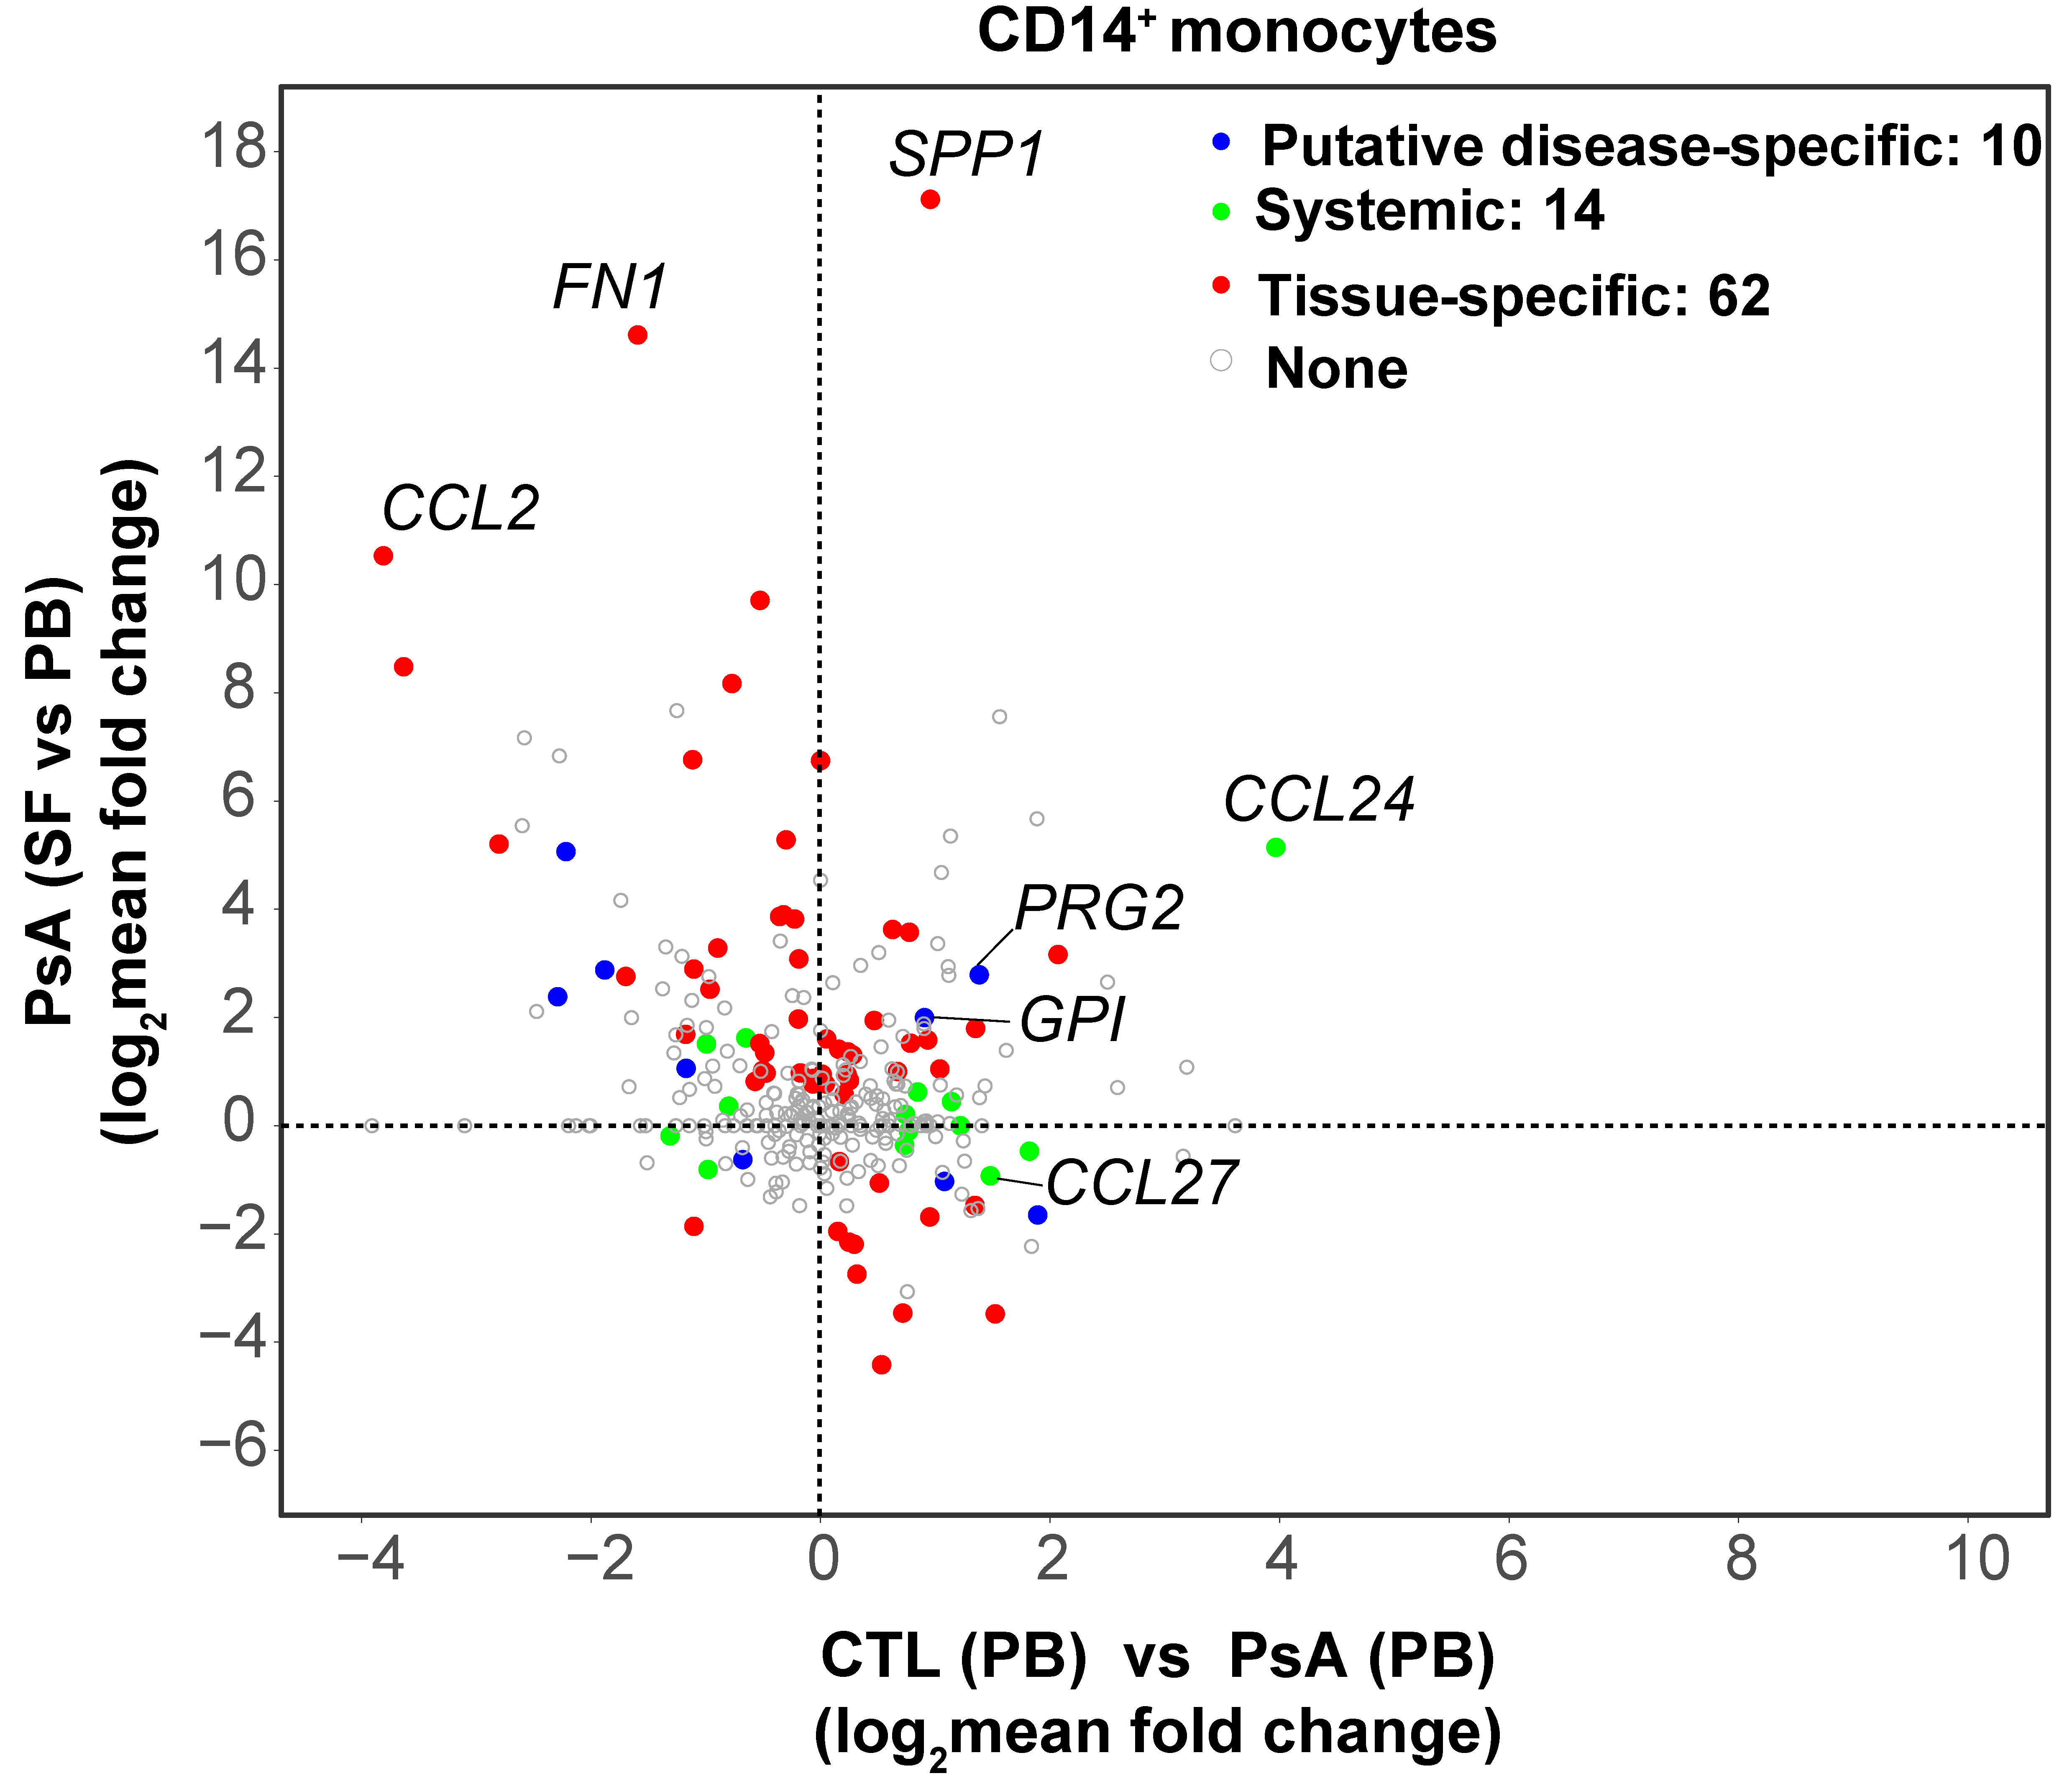
\includegraphics[width=\textwidth]{./Results3/pdfs/PSA_array_correlation_CD14_FC_HVPsA_vs_SFPBPsA}
\caption{\textbf{}}
% The percentage sign indicated that the other subfig goes side by side
\end{subfigure} \\
\begin{subfigure}{0.5\textwidth}
\centering
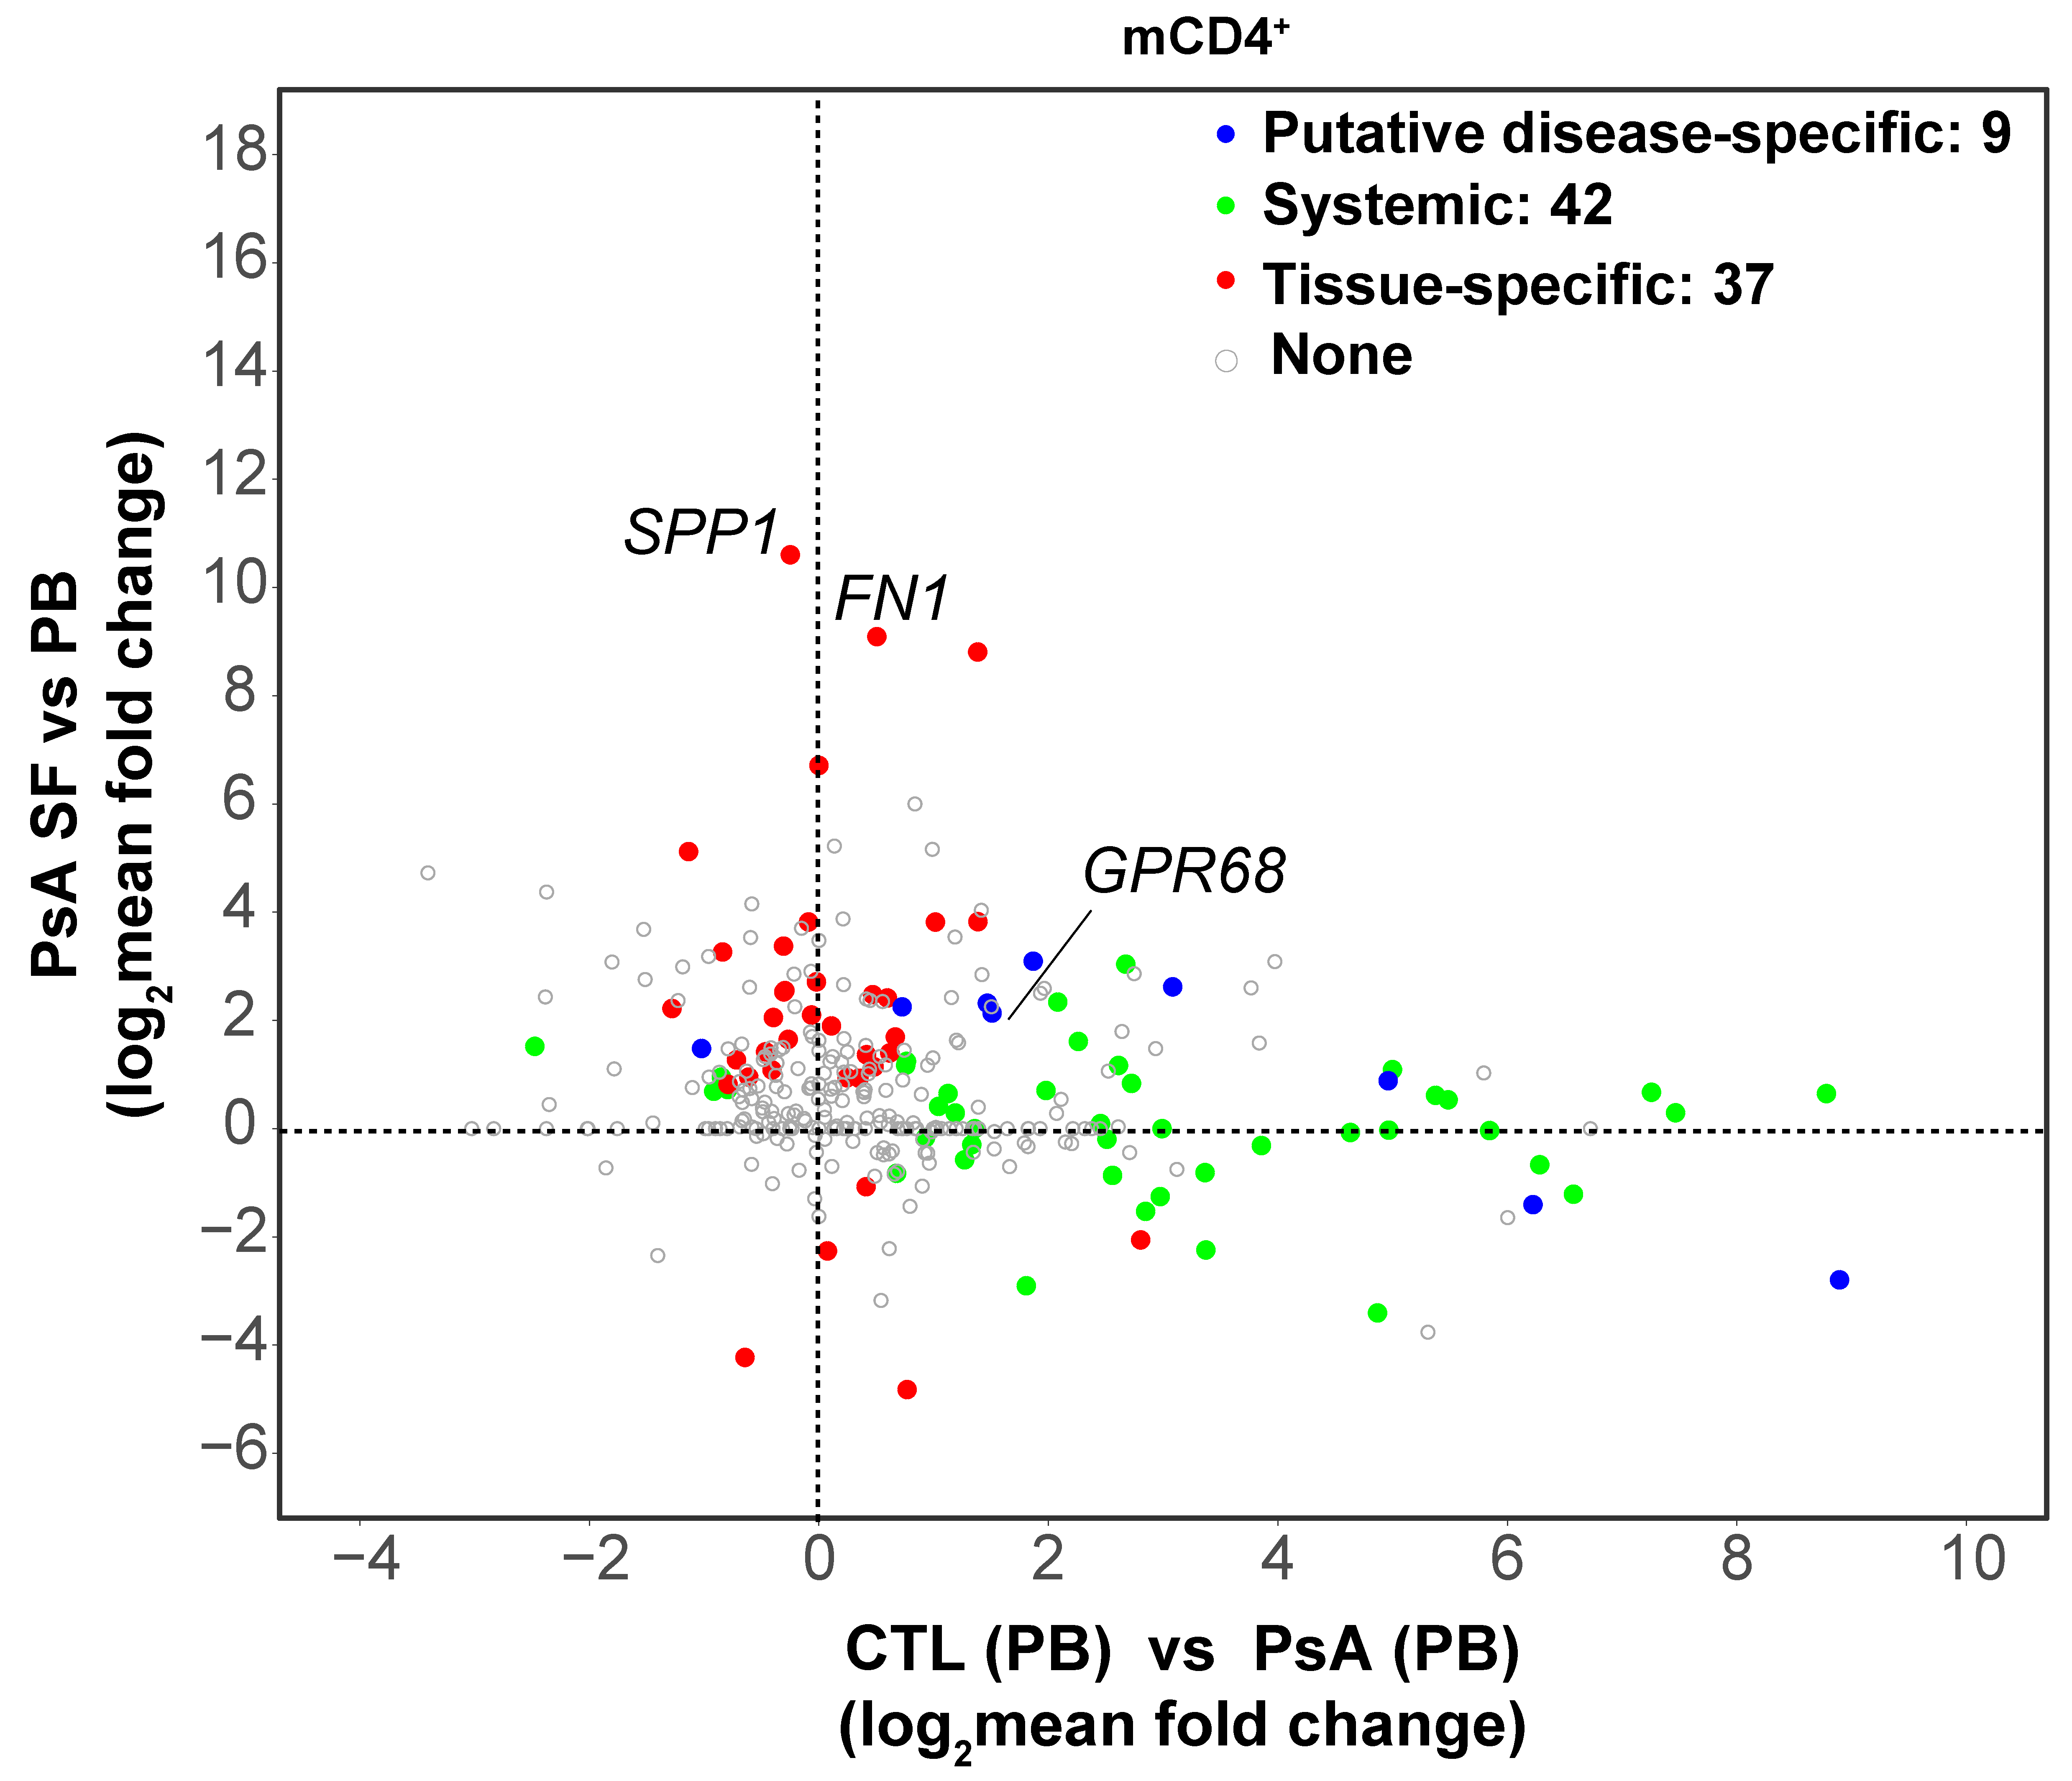
\includegraphics[width=\textwidth]{./Results3/pdfs/PSA_array_correlation_CD4_FC_HVPsA_vs_SFPBPsA}
\caption{\textbf{}}
\end{subfigure} %
\begin{subfigure}{0.5\textwidth}
\centering
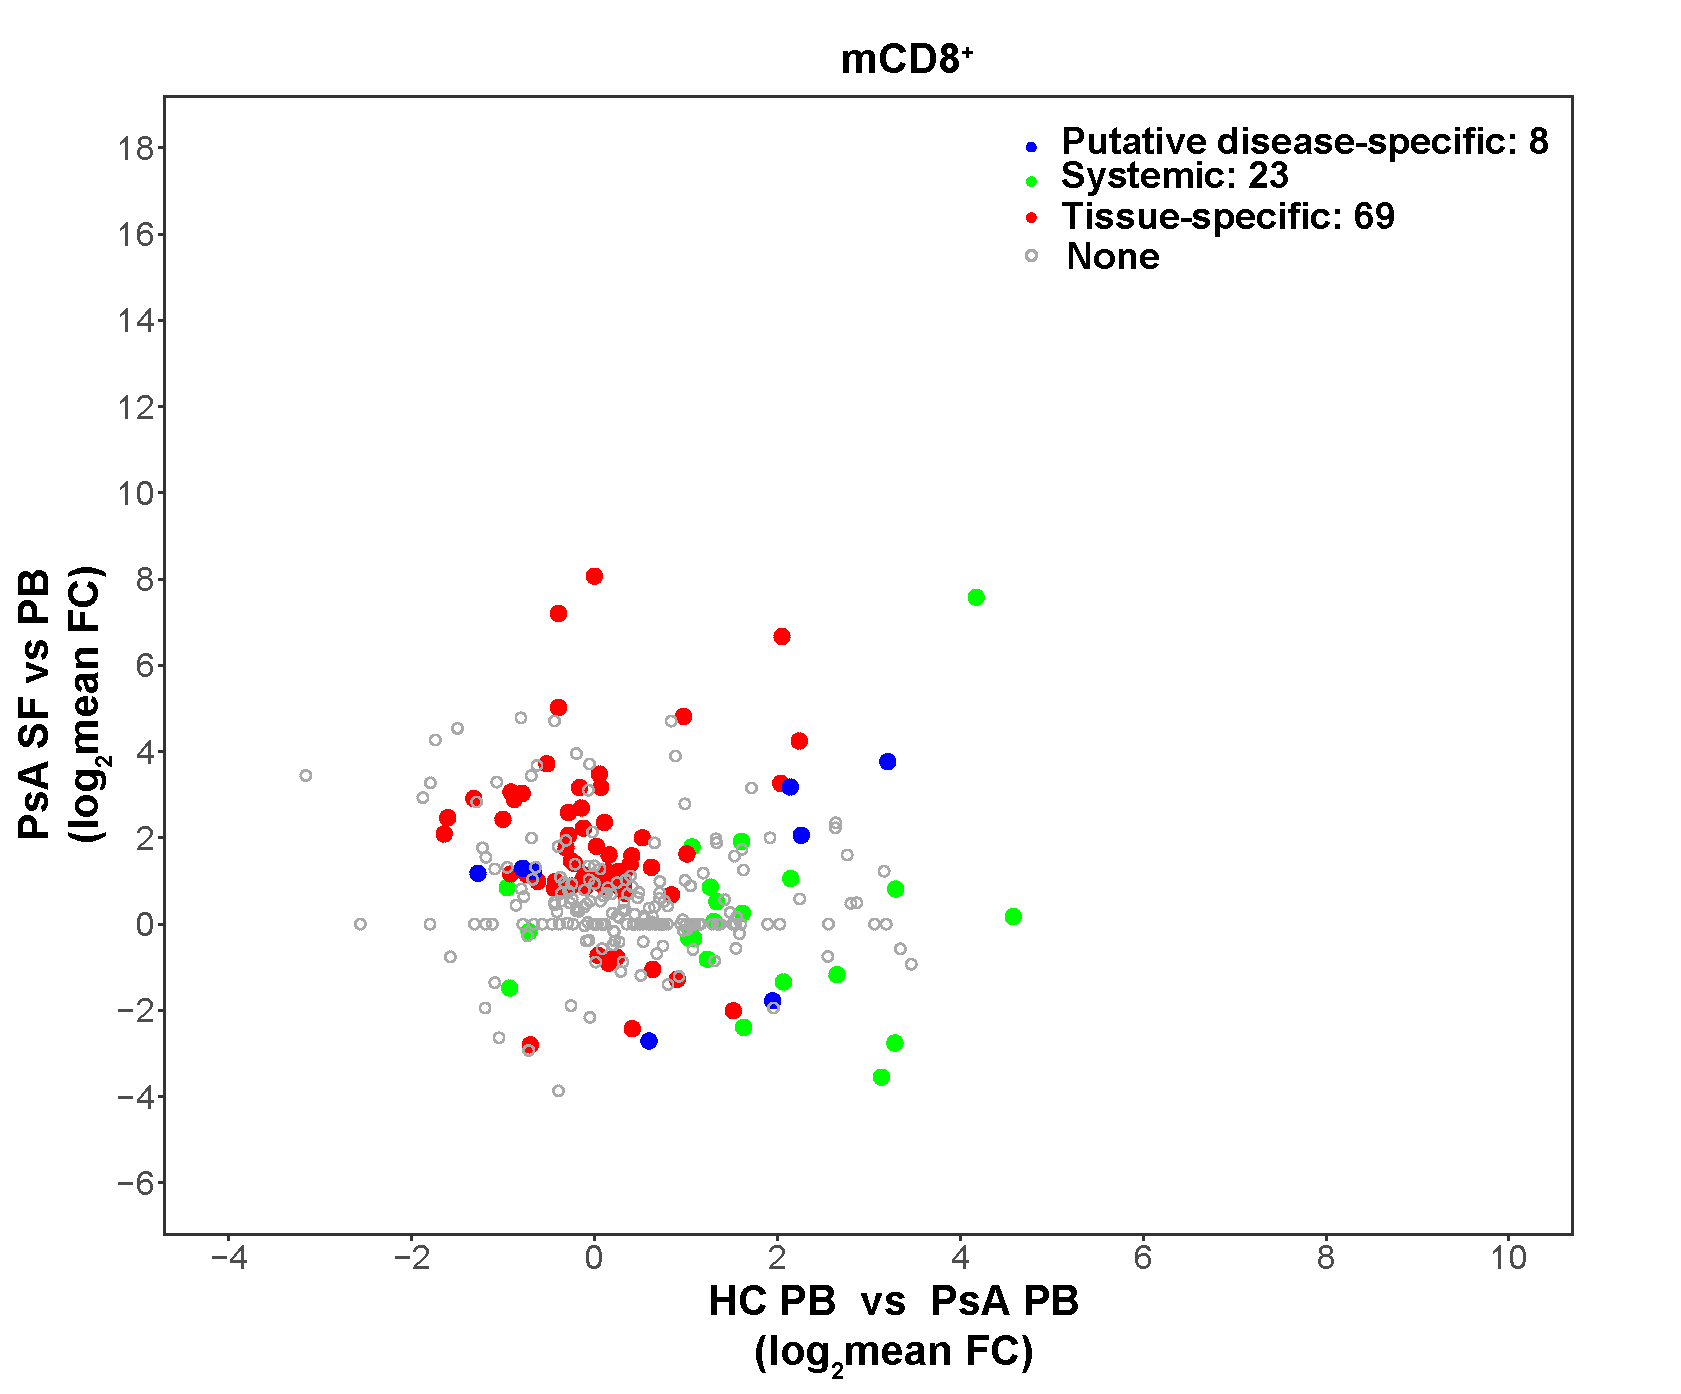
\includegraphics[width=\textwidth]{./Results3/pdfs/PSA_array_correlation_CD8_FC_HVPsA_vs_SFPBPsA}
\caption{\textbf{}}
\end{subfigure}
\caption[Expression changes in immune-relevant genes between SF and PB in CD14$^+$ monocytes, mCD4$^+$ and mCD4$^+$ cells.]{\textbf{Expression changes in immune-relevant genes between SF and PB in CD14$^+$ monocytes, mCD4$^+$ and mCD4$^+$ cells.}}
\label{fig:PSA_PCR_array_HC_FC_correlation}
\end{figure} 



\subsection{Mass cytometry reveals CD14$^+$ monocytes as the most active cytokine producing cells}

Measurement of cytokine production using mass cytometry was conducted in collaboration with Dr Hussein Al-Mossawi and Dr Nicole Yager. Cytokine production by CD14$^+$ monocytes, mCD4$^+$ T cells, mCD8$^+$ T cells and NK was quantified in SF and PB after incubation with BFA for 6 h. BFA blocks cytokine release and enables to measure the cell cytokine production rate in absence of any inflammatory stimuli, as previously explained in Chapter \ref{ch:Mat}(Figure \ref{figure:PSA_cytof_cytokines}). Following data QC, IL-2, IL-8, IFN-$\gamma$ and TNF-$\alpha$ were the cytokines consistently released with the most reliable quantification results within each of the manual gated cell type clusters. CD14$^+$ monocytes isolated from both, SF and PB, was the only active cell type in producing IFN-$\gamma$, IL-2 and IL-8. Nevertheless, no significant differences in the production (mean) of those three cytokines was observed in CD14$^+$ monocytes between SF and PB. On the other hand, only CD14$^+$ monocytes isolated from SF showed positive detectable mean levels of TNF-$\alpha$, which was undetectable in the PB counterpart cells. 

% IL8 production in CD4 https://www.ncbi.nlm.nih.gov/pubmed/7763239
% IL-8 monocytes and other cell types https://www.ncbi.nlm.nih.gov/pmc/articles/PMC4188125/
% TNFa in CD8 http://www.reproduction-online.org/content/141/2/249.full
\begin{figure}[htbp]
\centering
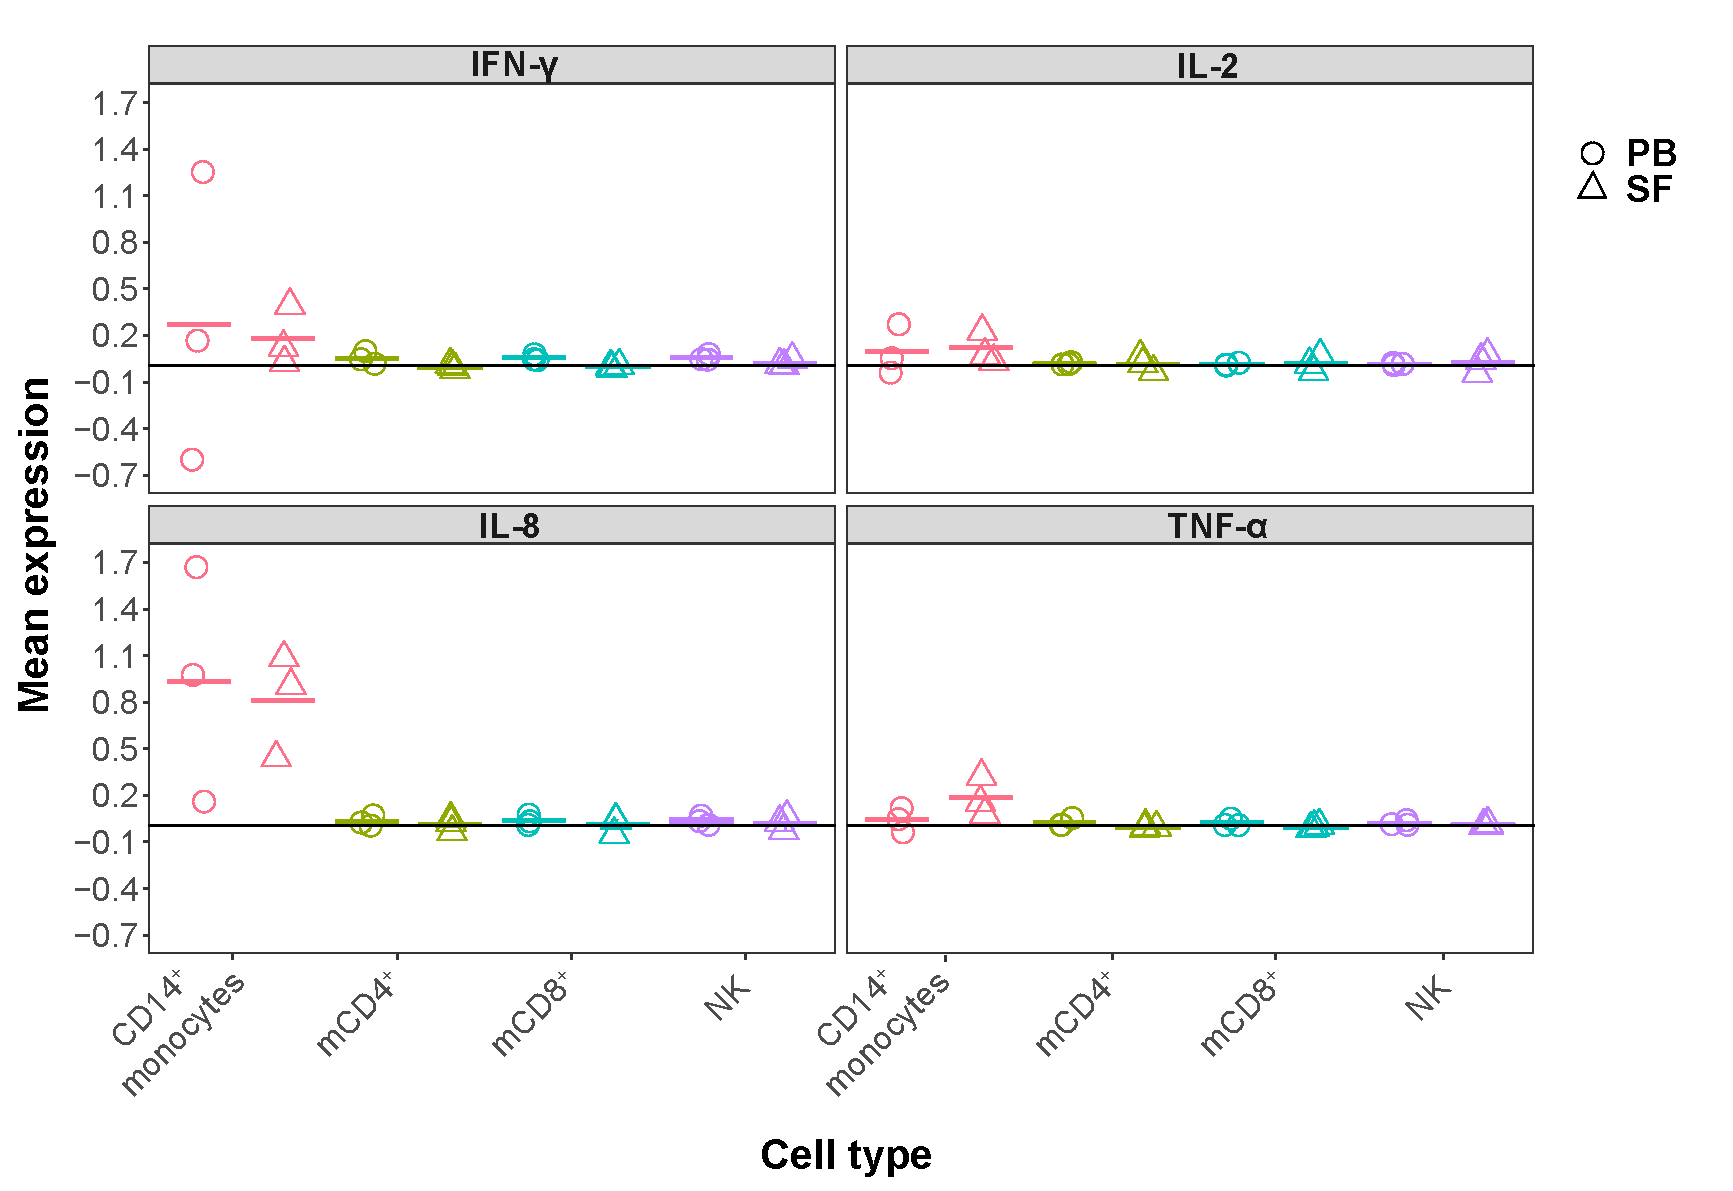
\includegraphics[width=0.8\textwidth]{./Results3/pdfs/CyTOF_ICS_cytokines_production_IL2_IL8_TNF_IFNg}
\caption[Mean expression of IL-2, IL-8, TNF-$\alpha$ and IFN-$\gamma$ in SF and PB from PsA patients.]{\textbf{Mean expression of IL-2, IL-8, TNF-$\alpha$ and IFN-$\gamma$ in SF and PB from PsA patients.} Expression levels quantified by mass cytometry. xxxx }
\label{fig:PSA_cytof_cytokines}
\end{figure}


The increased rate of TNF-$\alpha$ production by SF CD14$^+$ monocytes was reinforced when comparing the proportion of TNF-$\alpha$ positive cells after 6h of blocked cytokine secretion in each of the two tissues. The mass cytometry analysis of CD14$^+$ versus TNF-$\alpha$ signal showed a greater number of SF CD14$^+$ monocytes producing TNF$\alpha$ after 6 h of BFA treatment compared to PB for each of the three analysed patients (Figure \ref{figure:PsA_monocytes_percentage_TNFa} a). The basal (0h) percentage of CD14$^+$ monocytes positive for TNF-$\alpha$was negligible for all three patients in both, SF and PB (Figure \ref{figure:PsA_monocytes_percentage_TNFa} b). Conversely, upon inhibition of protein transport (6h), the percentage of CD14$^+$ monocytes producing TNF-$\alpha$ experienced an increase, ranging between 2 and 11.8\%, in SF whereas the increment in PB did not reach 1\%. This trend of increased percentage of SF CD14$^+$ monocytes TNF-$\alpha$ did not reach significance likely due to the small sample size. 
 
\bigskip
\begin{figure}[H]
\centering
\begin{subfigure}[b]{0.80\textwidth}
\centering 
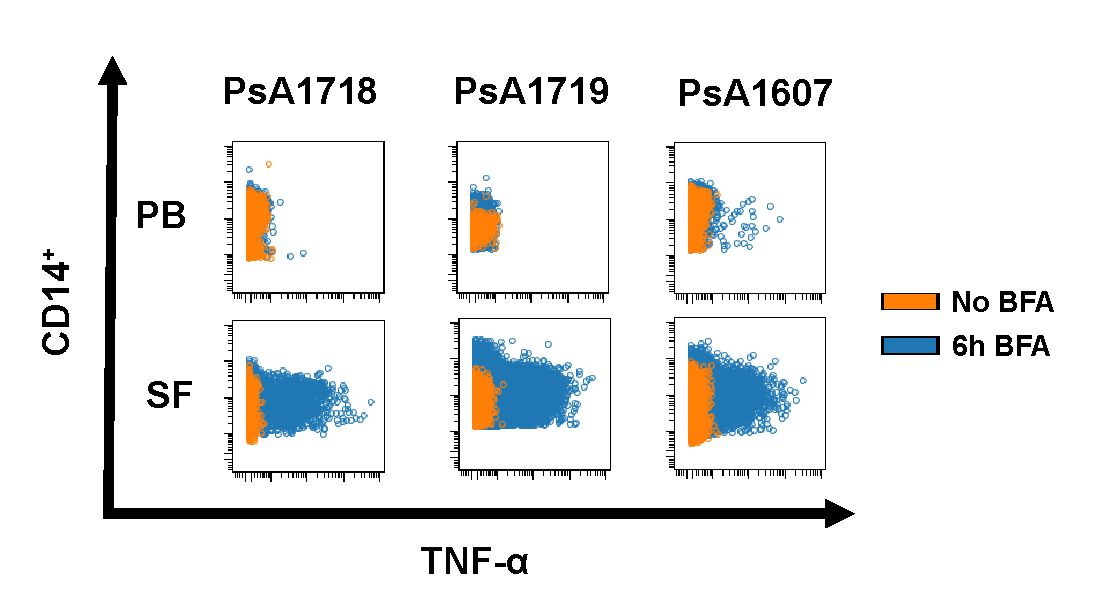
\includegraphics[width=\textwidth]{./Results3/pdfs/PSA_0h_6h_BFA_TNFa_mass_cytometry_PSA1718_PSA1719_PSA1607}
\caption{}
\end{subfigure}
~
\begin{subfigure}[b]{0.65\textwidth} 
%the [b] prevents offset in subcaptions
\centering
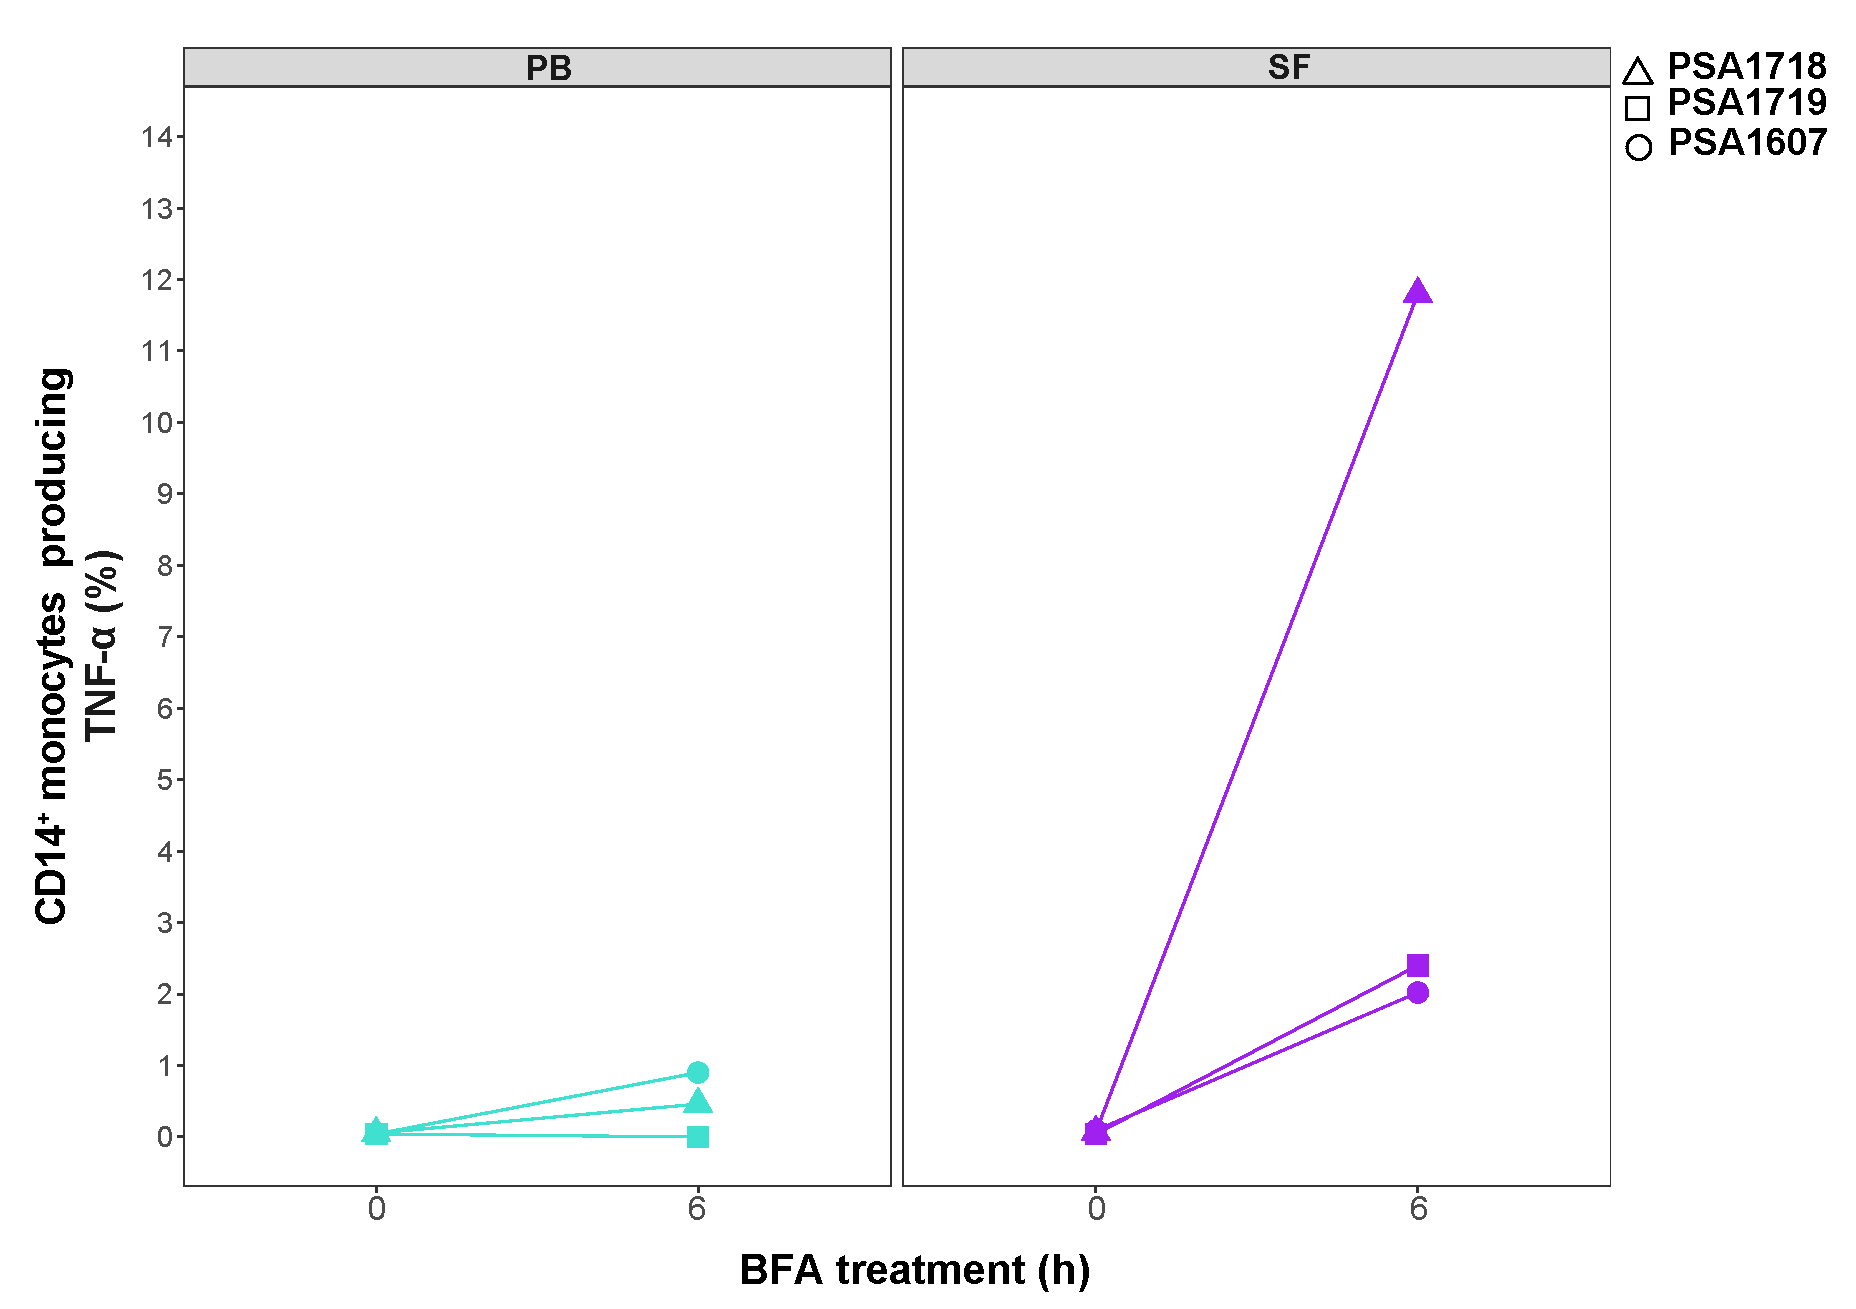
\includegraphics[width=\textwidth]{./Results3/pdfs/PSA_percent_monocytes_producing_TNFa_PB_and_SF}
\caption{}
\end{subfigure}
\caption[Mass cytometry analysis of TNF-$\alpha$ production in SF and PB by CD14$^+$ monocytes after protein transport blockade with BFA.]{\textbf{Differentially accessible regions located within gene bodies in CD14$^+$ monocytes and NK cells from PsA patients.} xxxx}
\label{figure:PsA_monocytes_percentage_TNFa}
\end{figure}


%This cytokine panel is representative of the four cell types of interest. TNF-$\alpha$ is released by all four cell types whereas IFN-$\gamma$ is mostly produced by lymphocytes and NK cells. Although IL-8 is mainly produced by fibroblasts and neutrophils, it is also secreted by monocytes and CD4$^+$ T cells, this last one being also the main source for IL-2 production. 






%%%%%%%%%%%%%%%%%%%%%%%%%%%%%%%%%%%%%%%%%%%%%%%%%%
\section{Discussion}
%
In Dolcino PSA vs HV SF comparison also detected more up genes than down in the array analysis
Say which cell types drive more the top changed gened

fGWAS analysis as Matthias did would be of interest but needs appropriate GWAS data
I am going to try using XGR to do some of this 

%NOD-like in PsA: https://www.ncbi.nlm.nih.gov/pmc/articles/PMC4792137/
%TLR in PsA: https://www.ncbi.nlm.nih.gov/pmc/articles/PMC2787278/

% SIGRR downregulation by LPS https://www.ncbi.nlm.nih.gov/pmc/articles/PMC4140261/
% CCL2 and CXCL10 in PsA